
\begin{partbacktext}
\part{Онтологические модели интерфейсов интеллектуальных компьютерных систем нового поколения}

\vspace{-3\baselineskip}

\begin{SCn}
	\scntext{аннотация}{Принципы организации и структура \textit{интерфейсов интеллектуальных компьютерных систем нового поколения}. Подход к реализации \textit{естественно-языковых интерфейсов интеллектуальных компьютерных систем нового поколения}, \textit{аудио} и \textit{речевых интерфейсов интеллектуальных компьютерных систем нового поколения}. Построение и использование трехмерного представления в различных задачах прикладных \textit{интеллектуальных компьютерных систем}, а также соответствующих систем позиционирования и ориентации в пространстве, описание такого представления, а также принципов его построения.}
	
	\bigskip
	
	\begin{scnrelfromlist}{подраздел}
		\scnitem{Глава~\ref{chapter_interfaces}~\nameref{chapter_interfaces}}
		\scnitem{Глава~\ref{chapter_nl_interfaces}~\nameref{chapter_nl_interfaces}}
		\scnitem{Глава~\ref{chapter_audio_interfaces}~\nameref{chapter_audio_interfaces}}
		\scnitem{Глава~\ref{chapter_3D_models}~\nameref{chapter_3D_models}}
	\end{scnrelfromlist}
\end{SCn}

\end{partbacktext}

\chapauthor{Садовский М.Е.}
\chapter{Общие принципы организации интерфейсов ostis-систем}
\chapauthortoc{Садовский М.Е.}
\label{chapter_interfaces}

\bigskip
\begin{SCn}
	
\begin{scnrelfromlist}{автор}
	\scnitem{Садовский М.~Е.}
\end{scnrelfromlist}
\bigskip

\scntext{аннотация}{В главе рассмотрены принципы организации \textit{интерфейсов интеллектуальных компьютерных систем нового поколения}. Ключевыми свойствами \textit{интерфейсов интеллектуальных компьютерных систем нового поколения} являются адаптивность и мультимодальность, что обеспечивает переход от парадигмы грамотного пользователя к парадигме равноправного сотрудничества пользователя с интеллектуальной системой, что позволяет повысить эффективность человеко-машинного взаимодействия. В главе рассматривается подход к обеспечению указанных свойств на основе онтологической модели интерфейса и онтологической модели процесса проектирования интерфейсов.}

\bigskip

\begin{scnrelfromlist}{подраздел}
	\scnitem{\ref{sec_analysis}~\nameref{sec_analysis}}	
	\scnitem{\ref{sec_proposed_ui_approach}~\nameref{sec_proposed_ui_approach}}
	\scnitem{\ref{sec_interface_user_actions}~\nameref{sec_interface_user_actions}}
	\scnitem{\ref{sec_messages}~\nameref{sec_messages}}
	\scnitem{\ref{sec_interfaces_actions_and_agents}~\nameref{sec_interfaces_actions_and_agents}}
\end{scnrelfromlist}

\bigskip

\begin{scnrelfromlist}{ключевое понятие}
	\scnitem{интерфейс}
	\scnitem{физический интерфейс}
	\scnitem{программный интерфейс}
	\scnitem{пользовательский интерфейс}
	\scnitem{интерфейс ostis-систем}
	\scnitem{адаптивный интерфейс}
	\scnitem{интеллектуальный интерфейс}
	\scnitem{мультимодальный интерфейс}
	\scnitem{компонент пользовательского интерфейса}
	\scnitem{интерфейсное действие пользователя}
	\scnitem{сообщение}
	\scnitem{решатель задач пользовательского интерфейса ostis-систем}
	\scnitem{интерпретатор sc-моделей пользовательских интерфейсов}
	\scnitem{интерпретатор пользовательских действий}
\end{scnrelfromlist}

\bigskip

\begin{scnrelfromlist}{ключевое отношение}
	\scnitem{инициируемое пользовательским интерфейсом действие*}
\end{scnrelfromlist}

\bigskip

\begin{scnrelfromlist}{ключевое знание}
	\scnitem{Предметная область пользовательских интерфейсов}
	\scnitem{Предметная область компонентов интерфейса}
\end{scnrelfromlist}

\bigskip

\begin{scnrelfromlist}{библиографическая ссылка}
	\scnitem{}
\end{scnrelfromlist}
\end{SCn}

\section*{Введение в Главу \ref{chapter_interfaces}}

Организация взаимодействия пользователей с компьютерными системами (в том числе и с интеллектуальными компьютерными системами) оказывает существенное влияние на эффективность автоматизации человеческой деятельности, пользовательский опыт и уровень удовлетворенности пользователей. 

Одним из ключевых свойств интеллектуальных компьютерных систем нового поколения является их \myuline{интероперабельность} --- способность к эффективному взаимодействию. Такие системы являются автономными и самодостаточными субъектами деятельности наравне с человеком. Однако, в основе современной организации взаимодействия пользователя с компьютерной системой лежит парадигма \myuline{грамотного пользователя}, который знает, как управлять системой и несёт полную ответственность за качество взаимодействия с ней. Многообразие форм и видов интерфейсов приводит к необходимости пользователя адаптироваться к каждой конкретной системе, обучаться принципам взаимодействия с ней для решения необходимых ему задач.

На современном этапе развития Искусственного интеллекта для повышения эффективности взаимодействия необходим переход от парадигмы грамотного управления используемым инструментом к парадигме \textbf{равноправного сотрудничества, партнёрскому взаимодействию} интеллектуальной компьютерной системы со своим пользователем. Дружественность пользовательского интерфейса должна заключаться в адаптивности системы к особенностям и квалификации пользователя, исключении любых проблем для пользователя в процессе диалога с интеллектуальной компьютерной системой, в перманентной заботе о совершенствовании коммуникационных навыков пользователя. Следовательно, необходимо отойти от привычной адаптации пользователя к системе (путем обучения ее использованию) в сторону адаптации самого интерфейса под цели, задачи и характеристики конкретного пользователя в режиме реального времени (см. \scncite{fomina}).

\section{Анализ и проблемы существующих принципов организации интерфейсов}
\label{sec_analysis}

\textit{интерфейс} --- совокупность технических, программных и методических (протоколов, правил, соглашений) средств, обеспечивающих обмен информацией между пользователем и устройствами и программами, а также между устройствами и другими устройствами и программами. В широком смысле слова, это способ (стандарт) взаимодействия между объектами. Интерфейс в техническом смысле слова задаёт параметры, процедуры и характеристики взаимодействия объектов.

\textit{интерфейсы} бывают разных видов. Они отличаются по характеру систем, которые взаимодействуют между собой; реализацией и функциями.

Вне зависимости от типа интерфейса, взаимодействие компьютерной системы с окружающей средой происходит при помощи \textit{сенсоров} и \textit{эффекторов}.
Ключевая задача \textit{интерфейса} --- обеспечение эффективного взаимодействия с внешними субъектами (пользователями, другими \textit{ostis-системами}, другими традиционными компьютерными системами).

Принято выделять следующие виды \textit{интерфейсов}:
\begin{textitemize}
	\item \textit{физический интерфейс};
	\item \textit{программный интерфейс};
	\item \textit{пользовательский интерфейс}.
\end{textitemize}

\textit{физический интерфейс} позволяет преобразовать сигналы и передать их от одного компонента оборудования к другому и определяется набором электрических связей и характеристиками сигналов.

\textit{программный интерфейс} предназначен для обмена информацией между компонентами вычислительной системы и задает набор необходимых процедур, их параметров и способов обращения.

\textit{пользовательский интерфейс} --- один из наиболее важных компонентов компьютерной системы. Представляет собой совокупность аппаратных и программных средств, обеспечивающих обмен информацией между пользователем и компьютерной системой.

В контексте данной главы основное внимание будет уделено \textit{пользовательским интерфейсам}, другие виды интерфейсов являются объектами будущих исследований.

Ключевыми проблемами современных пользовательских интерфейсов являются:
\begin{textitemize}
	\item \myuline{необходимость пользователя обучаться принципам взаимодействия} с каждой конкретной системой;
	\item \myuline{отсутствие партнерского взаимодействия} между пользователем и системой (система является объектом управления со стороны пользователя), что приводит к необходимости пользователя быть постоянным инициатором взаимодействия;
	\item \myuline{отсутствие адаптации системы} к особенностям каждого конкретного пользователя и окружающей среды для максимально комфортного взаимодействия пользователя с системой.
\end{textitemize}

\textit{интерфейс интеллектуальных компьютерных систем нового поколения} должен обеспечивать взаимодействие с пользователем на \myuline{равноправной основе, уметь адаптироваться к его особенностям,} а также \myuline{воспринимать различные типы} \myuline{ввода информации}. Для организации такого взаимодействия используются термины \textit{адаптивного}, \textit{интеллектуального} и \textit{мультимодального интерфейса}.

\textit{адаптивный интерфейс} --- \textit{пользовательский интерфейс}, который изменяется на основе потребностей пользователя или контекста использования.

Как правило, контекст использования состоит из знаний о \myuline{пользователе, платформе и среде}, как показано на рисунке \nameref{fig:use_context} (см. \scncite{jamil_hussain}).

\begin{figure}[H]
	\centering
	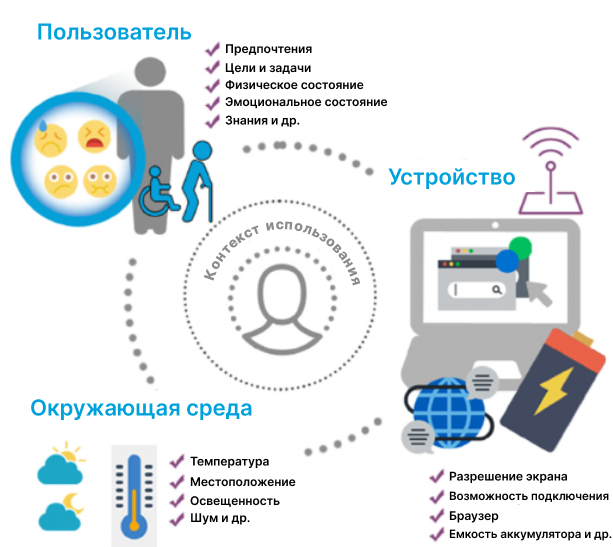
\includegraphics[scale=0.5]{author/part4/figures/user-context.png}
	\caption{Контекст использования системы}
	\label{fig:use_context}
\end{figure}

Настройка функциональных возможностей и параметров интерфейса может осуществляться либо вручную самим пользователем, либо автоматически системой на основании имеющейся информации о пользователе. Таким образом, следует различать адаптивные и адаптируемые системы, эти термины не являются синонимами, хотя в литературе довольно часто можно встретить подмену данных понятий (см. \scncite{valeev2}).

В адаптируемых системах любая адаптация является предопределенной и может изменяться пользователями перед запуском системы. В адаптивных же системах, напротив, любая адаптация является динамической, то есть происходит в то же время, когда пользователь взаимодействует с системой, и зависит от поведения пользователя. Но система также может быть адаптируемой и адаптивной одновременно (см. \scncite{Montero}).
Недостаток ручного редактирования интерфейса заключается в необходимости пользователя быть достаточно хорошо знакомым, как с самой системой, так и со средствами, позволяющими изменять ее \textit{интерфейс}.

Также в литературе можно встретить термин \textit{``адаптированный интерфейс''}. 

\textit{адаптированный интерфейс} --- это \textit{пользовательский интерфейс}, который адаптирован к конечному пользователю при проектировании и не изменяется во время эксплуатации системы (см. \scncite{Schlungbaum1997IndividualUI}).

\textit{интеллектуальный интерфейс} --- \textit{пользовательский интерфейс}, который может предположить дальнейшие действия пользователей и представить информацию на основе этого предположения. Можно заметить, что понятия интеллектуальный и адаптивный интерфейс имеют отличия. Однако, в различных статьях эти понятия рассматриваются как синонимы.

\textit{мультимодальный интерфейс} --- \textit{пользовательский интерфейс}, предназначенный для обработки двух или более комбинированных режимов пользовательского ввода, таких как речь, перо, касание, ручные жесты и взгляд, скоординированным образом с выводом мультимедийной системы.

Взаимодействие с большей частью традиционных компьютерных систем происходит с помощью клавиатуры и мыши (тачпада, стилуса). Пользовательский интерфейс таких систем, как правило, не хранит информацию о модели пользователя, историю его действий и так далее. Традиционный пользовательский интерфейс также не содержит модуль адаптации. На рисунке \nameref{fig:traditional_ui} представлена структура традиционного пользовательского интерфейса (см.\scncite{OSTIS2022Sadovski}).

\begin{figure}[H]
	\centering
	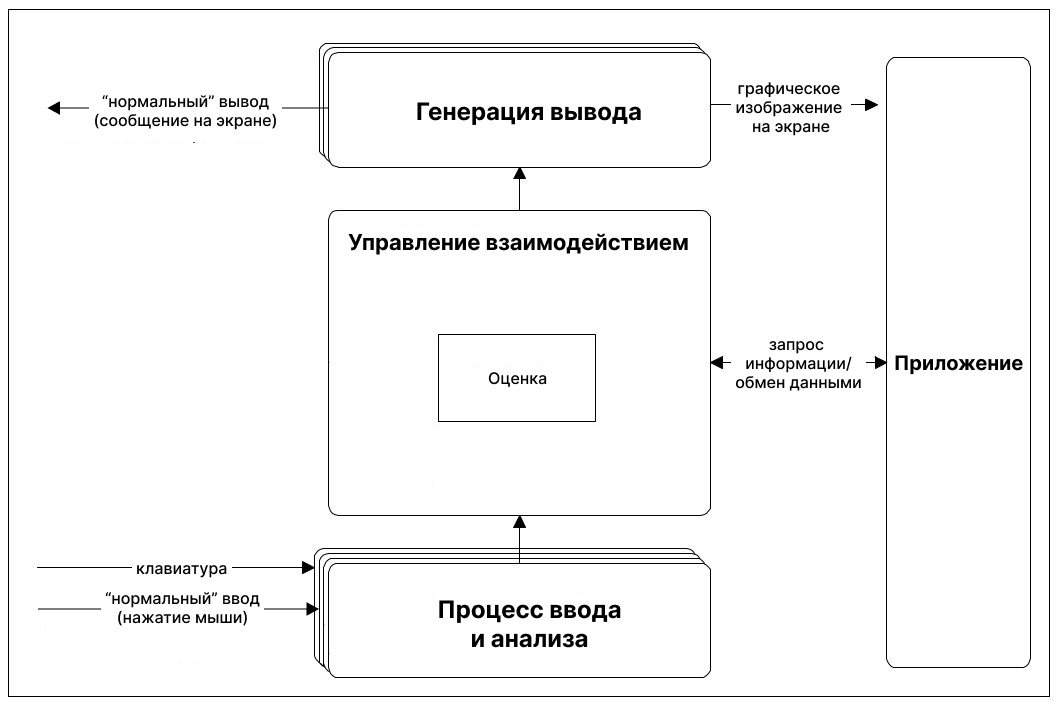
\includegraphics[scale=0.4]{author/part4/figures/traditional_ui.png}
	\caption{Структура традиционного пользовательского интерфейса}
	\label{fig:traditional_ui}
\end{figure}

Общая архитектура адаптивного интеллектуального мультимодального пользовательского интерфейса в свою очередь, как правило, выглядит так, как представлено на рисунке \nameref{fig:adaptive_ui}.

\begin{figure}[H]
	\centering
	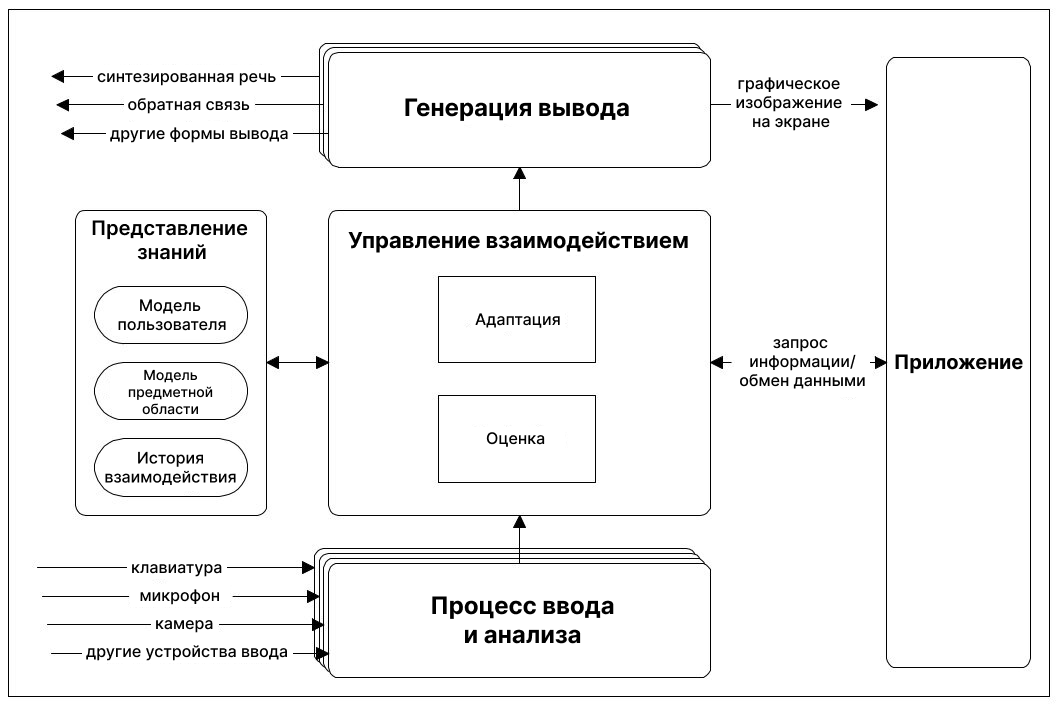
\includegraphics[scale=0.4]{author/part4/figures/adaptive_ui.png}
	\caption{Структура адаптивного интеллектуального мультимодального пользовательского интерфейса}
	\label{fig:adaptive_ui}
\end{figure}

Среди современных средств создания адаптивных пользовательских интерфейсов можно выделить следующие средства, представленные на рисунке \nameref{fig:adaptive_ui_tools} (см. \scncite{context}).

\begin{figure}[H]
	\centering
	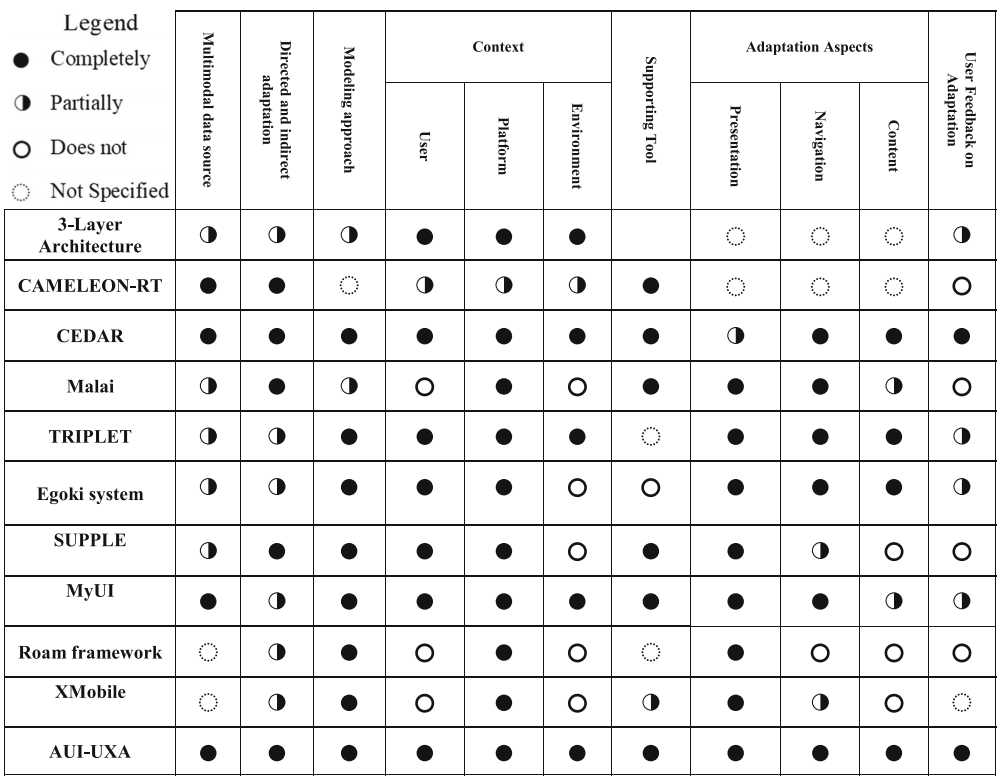
\includegraphics[scale=0.4]{author/part4/figures/adaptive_ui_tools.png}
	\caption{Существующие средства создания адаптивных пользовательских интерфейсов}
	\label{fig:adaptive_ui_tools}
\end{figure}

Вне зависимости от средств создания \textit{адаптивных интеллектуальных мультимодальных пользовательских интерфейсов} такие системы должны эффективно хранить и обрабатывать знания о пользователе, взаимодействии с ним и другую необходимую информацию. Большинство таких систем используют онтологическую модель для хранения информации для адаптации пользовательского интерфейса. Именно онтологический подход позволяет:
\begin{textitemize}
	\item создать наиболее полное \myuline{унифицированное описание} различных аспектов пользовательского интерфейса;
	\item \myuline{легко интегрировать} различные аспекты \textit{пользовательского интерфейса};
	\item \myuline{упростить повторное использование} модели интерфейса.
\end{textitemize}

В рамках онтологического подхода принято выделять онтологии и предметные области. База знаний адаптивного интеллектуального мультимодального интерфейса должна включать как минимум следующие предметные области:
\begin{textitemize}
	\item \textit{Предметную область и онтологию модели пользователя}; 
	\item \textit{Предметную область и онтологию компонентов интерфейса};
	\item \textit{Предметную область и онтологию интерфейсных действий};
	\item \textit{Предметную область и онтологию контекста использования}.
\end{textitemize}

Среди существующих \textit{онтологий модели пользователя} можно выделить онтологию GUMO (см. \scncite{Heckmann}), в рамках которой выделяют:
\begin{textitemize}
	\item физиологическое состояние --- может измениться за секунды;
	\item психическое состояние --- может измениться за минуты;
	\item эмоциональное состояние --- может измениться за часы;
	\item характер --- может измениться за месяцы;
	\item личность --- может измениться за годы;
	\item демография --- обычно не может измениться.
\end{textitemize}

В работе \scncite{paulheim} рассматривается \textit{онтология компонентов интерфейса}, на верхнем уровне которой рассматриваются следующие типы компонентов:
\begin{textitemize}
	\item компонент пользовательского интерфейса для отображения;
	\item декоративный компонент пользовательского интерфейса;
	\item интерактивный компонент пользовательского интерфейса;
	\item компонент ввода данных;
	\item компонент для манипуляции отображением;
	\item компонент для запуска операций;
	\item контейнер;
	\item окно;
	\item модальное окно;
	\item немодальное окно.
\end{textitemize}

В данную онтологию также можно включить классы свойств компонента, которые определяют оформление внешнего вида интерфейсных элементов, начиная от простых, таких как шрифт, цвет, размер элементов, до составных, содержащих наборы интерфейсных решений (см. \cite{gribova_2022}).

Классификация \textit{интерфейсных действий} представлена в \scncite{paulheim} и содержит следующие основные классы:
\begin{textitemize}
	\item действие мышью;
	\item действие речью;
	\item действие осязания;
	\item действие прикосновения.
\end{textitemize}


\textit{Онтология контекста использования} рассматривается в работе \scncite{dream} и описывает:
\begin{textitemize}
	\item Статус пользователей:
	\begin{textitemize}
		\item Движение (стояние, сидение, ходьба);
		\item Возможность слушать (да, нет);
		\item Возможность печатать (да, нет);
		\item Возможность говорить (да, нет);
		\item Возможность читать (да, нет);
	\end{textitemize}
	\item Естественная среда:
	\begin{textitemize}
		\item Освещение (яркий, умеренно освещенный, темный);
		\item Шум (шумный, тихий);
		\item Ветер (сильный, слабый, безветрие);
		\item Погода (солнечно, облачно, дождливо);
		\item Температура (жарко, тепло, холодно);
		\item Местоположение (в офисе, в аэропорту, на улице, в библиотеке, дома, в торговом центре);
	\end{textitemize}
	\item Особенности устройства:
	\begin{textitemize}
		\item Размер экрана (большой, маленький);
		\item Тип экрана (монохромный, цветной);
		\item Клавиатура (большая, маленькая, виртуальная).
	\end{textitemize}
\end{textitemize}

Для управления взаимодействием пользователя с системой принято использовать \myuline{интеллектуальные агенты}.

\textit{интеллектуальный агент} способен выполнять гибкое автономное действие для достижения своих целей. Согласно данному определению, гибкость означает:
\begin{textitemize}
	\item Реактивность: интеллектуальные агенты способны воспринимать свою среду и реагировать в своевременном режиме на изменения в ней, чтобы удовлетворить свои цели проектирования;
	\item Проактивность: интеллектуальные агенты способны проявлять целенаправленное поведение, инициируя действия для достижения своих целей проектирования;
	\item Социальная способность: интеллектуальные агенты способны взаимодействовать с другими агентами (и, возможно, людьми) с целью удовлетворения своих целей проектирования.
\end{textitemize}
\textit{интеллектуальные агенты} направлены на единственную цель, но обладают большим знанием о рассуждении в пределах своей деятельности. Умение использовать другие ресурсы (других агентов), предпочтения пользователя или клиента и другие способности являются признаками интеллектуального агента.

В результате проведенного анализа можно сделать следующие выводы:
\begin{textitemize}
	\item Для перехода к \myuline{\textit{парадигме равноправного сотрудничества пользователя и системы}} интерфейсы должны быть адаптивными, интеллектуальными и мультимодальными. Существующие решения позволяют проектировать такие интерфейсы, однако имеют ряд недостатков, которые будут представлены далее.
	\item Структура \textit{интеллектуальных интерфейсов} включает базу знаний, модуль управления взаимодействием пользователя с системой.
	\item При проектировании базы знаний активно применяется онтологический подход и уже реализованы некоторые онтологии, которые используются при проектировании интеллектуальных интерфейсов.
	\item Модуль управления взаимодействием пользователя с системой, как правило, реализуется на основе многоагентного подхода.
\end{textitemize} 

Среди недостатков существующих решений можно выделить:
\begin{textitemize}
	\item Существующие решения, как правило, предусматривают \myuline{вопросно-ответный принцип взаимодействия}.
	\item Актуальной остается \myuline{проблема совместимости интеллектуального интерфейса с интеллектуальной системой}, для которой он создается, в силу различий используемых средств и методов при проектировании и реализации.
	\item Актуальной остается \myuline{проблема совместимости компонентов интеллектуального интерфейса} (база знаний и модуль управления взаимодействием) между собой.
\end{textitemize}

Для устранения недостатков существующих решений предлагается использовать онтологический подход на основе семантической модели при проектировании и реализации \textit{адаптивного интеллектуального мультимодального пользовательского интерфейса}, принципы которого будут рассмотрены далее.

\section{Предлагаемый подход к организации интерфейсов ostis-систем}
\label{sec_proposed_ui_approach}

Для организации \textit{интерфейса ostis-систем} предлагаются следующие принципы:
\begin{textitemize}
	\item Под \textit{пользовательским интерфейсом ostis-системы} понимается специализированная \textit{ostis-система}, ориентированная на решение интерфейсных задач, и имеющая в своем составе базу знаний и решатель задач пользовательского интерфейса ostis-системы. Таким образом обеспечивается совместимость \textit{ostis-системы} и ее \textit{пользовательского интерфейса}.
	\item Для решения задачи построения пользовательского интерфейса в базе знаний \textit{пользовательского интерфейса ostis-системы} содержится sc-модель \textit{компонентов пользовательского интерфейса}, \textit{интерфейсных действий пользователей}, а также классификация \textit{пользовательских интерфейсов} в целом.
	\item Решатель задач \textit{пользовательского интерфейса ostis-системы} основан на многоагентном подходе, а сами агенты имеют возможность инициирования действий и сообщений пользователю и другим агентам.
	\item При проектировании \textit{пользовательского интерфейса ostis-системы} используется компонентный подход, который предполагает представление всего интерфейса приложения в виде отдельных специфицированных компонентов, которые могут разрабатываться и совершенствоваться независимо.
	\item Каждый компонент \textit{пользовательского интерфейса ostis-системы} является внешним отображением определенного элемента из базы знаний, что позволяет использовать их в качестве аргументов пользовательских команд и правильно трактовать прагматику и семантику объектов интерфейсной деятельности, легко изменять интерфейс системы даже во время ее эксплуатации, позволяет пользователю задавать системе вопросы касательно любого из компонентов интерфейса.
	\item Модель \textit{пользовательского интерфейса ostis-системы} строится независимо от реализации платформы интерпретации такой модели, что позволяет легко переносить разработанную модель на разные платформы.
	\item Описание модели базы знаний и решателя задач \textit{пользовательского интерфейса ostis-системы} предлагается осуществлять на основе универсального унифицированного языка представления знаний, что обеспечит совместимость между этими компонентами.
\end{textitemize}

\textit{пользовательский интерфейс ostis-системы} является адаптивным интеллектуальным мультимодальным пользовательским интерфейсом, структура которого представлена на рисунке \nameref{fig:ostis_ui_structure}.

\begin{figure}[H]
	\centering
	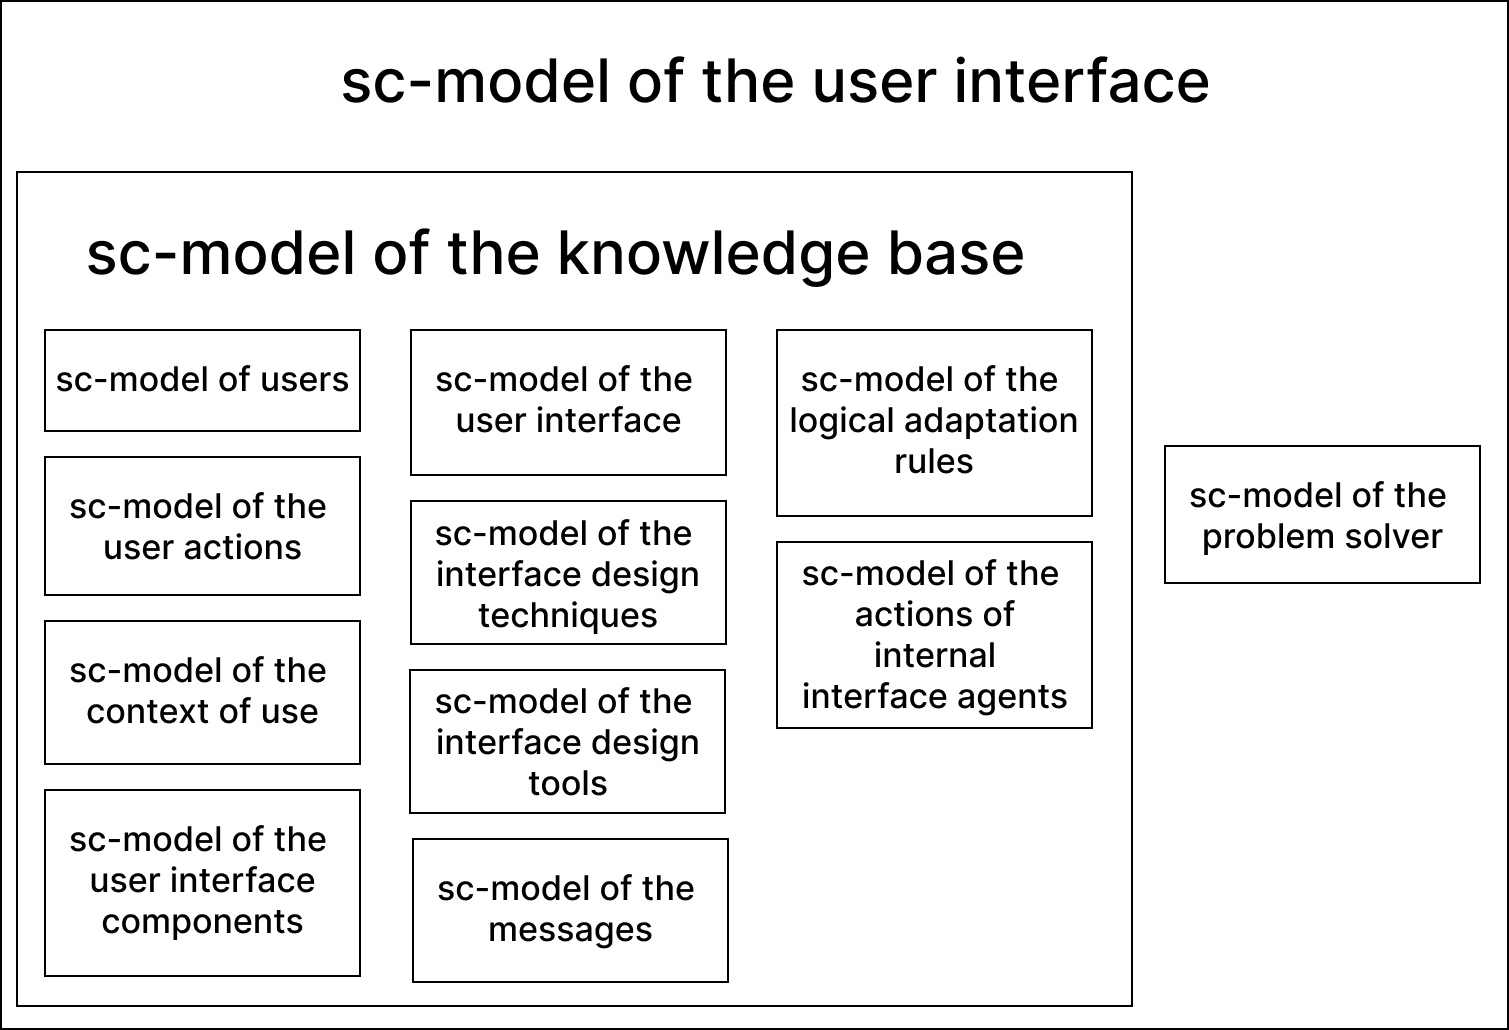
\includegraphics[scale=0.3]{author/part4/figures/ui_model.png}
	\caption{Структура пользовательского интерфейса ostis-системы}
	\label{fig:ostis_ui_structure}
\end{figure}

\textit{Предметная область пользовательских интерфейсов} представляет собой формализованную типологию пользовательских интерфейсов. Пример фрагмента данной предметной области в базе знаний пользовательского интерфейса будет выглядеть следующим образом.

\begin{SCn}
	\scnheader{интерфейс}
	\scnidtf{совокупность технических, программных и методических (протоколов, правил, соглашений) средств, обеспечивающих обмен информацией между пользователем и устройствами и программами, а также между устройствами и другими устройствами и программами. В широком смысле слова, это способ (стандарт) взаимодействия между объектами. Интерфейс в техническом смысле слова задаёт параметры, процедуры и характеристики взаимодействия объектов}
\end{SCn}

\begin{SCn}
	
	\scnheader{интерфейс}
	\begin{scnrelfromset}{разбиение}
			\scnitem{пользовательский интерфейc}
			\begin{scnindent}
					\scnidtf{один из наиболее важных компонентов компьютерной системы. Представляет собой совокупность аппаратных и программных средств, обеспечивающих обмен информацией между пользователем и компьютерной системой.}
				\end{scnindent}
			\scnitem{программный интерфейс}
			\begin{scnindent}
					\scnidtf{система унифицированных связей, предназначенных для обмена информацией между компонентами вычислительной системы. Программный интерфейс задает набор необходимых процедур, их параметров и способов обращения.}
				\end{scnindent}
			\scnitem{физический интерфейс}
			\begin{scnindent}
					\scnidtf{устройство, преобразующее сигналы и передающее их от одного компонента оборудования к другому. Физический интерфейс определяется набором электрических связей и характеристиками сигналов.}
				\end{scnindent}
		\end{scnrelfromset}
	
\end{SCn}

\begin{SCn}
	\scnheader{адаптивный интерфейс}
	\scnidtf{\textit{пользовательский интерфейс}, который изменяется на основе потребностей пользователя или контекста}
\end{SCn}

\begin{SCn}
	\scnheader{интеллектуальный интерфейс}
	\scnidtf{\textit{пользовательский интерфейс}, который может предположить дальнейшие действия пользователей и представить информацию на основе этого предположения}
\end{SCn}

\begin{SCn}
	\scnheader{мультимодальный интерфейс}
	\scnidtf{\textit{пользовательский интерфейс}, предназначенный для обработки двух или более комбинированных режимов пользовательского ввода, таких как речь, перо, касание, ручные жесты и взгляд, скоординированным образом с выводом мультимедийной системы}
\end{SCn}

\begin{SCn}
	
	\scnheader{пользовательский интерфейс}
	\scnsuperset{командный пользовательский интерфейс}
	\begin{scnindent}
			\scnidtf{\textit{пользовательский интерфейс}, при котором обмен информацией между компьютерной системой и пользователем осуществляется путем написания текстовых инструкций или команд}
		\end{scnindent}		
	\scnsuperset{WIMP-интерфейс}
	\begin{scnindent}
			\scnidtf{Window, Image, Menu, Pointer --- интерфейс}
			\scnidtf{Окно, Образ, Меню, Указатель --- интерфейс}
			\scnidtf{\textit{пользовательский интерфейс}, при котором обмен информацией между компьютерной системой и пользователем осуществляется в форме диалога при помощи окон, меню и других элементов управления}
			\begin{scnindent}
					\scnsuperset{пользовательский интерфейс ostis-системы}
				\end{scnindent}	
		\end{scnindent}
	\scnsuperset{SILK-интерфейс}
	\begin{scnindent}
			\scnidtf{Speech, Image, Language, Knowledge --- интерфейс}
			\scnidtf{Речь, Образ, Язык, Знание --- интерфейс}
			\scnidtf{\textit{пользовательский интерфейс}, наиболее приближенный к естественной для человека форме общения. Компьютерная система находит для себя команды, анализируя человеческую речь и находя в ней ключевые фразы. Результат выполнения команд преобразуется в понятную человеку форму, например, в естественно-языковую форму или изображение.}
			\scnsuperset{естественно-языковой интерфейc}
			\begin{scnindent}
					\scnidtf{SILK-интерфейс, обмен информацией между компьютерной системой и пользователем в котором происходит за счёт диалога. Диалог ведётся на одном из естественных языков}
				\end{scnindent}			
			\begin{scnindent}
					\scnsuperset{речевой интерфейc}
					\begin{scnindent}
							\scnidtf{SILK-интерфейс, обмен информацией в котором происходит за счёт диалога, в процессе которого компьютерная система и пользователь общаются с помощью речи. Данный вид интерфейса наиболее приближен к естественному общению между людьми}
						\end{scnindent}
				\end{scnindent}
		\end{scnindent}
	
\end{SCn}

\bigskip

\textit{Предметная область пользователя}, \textit{Предметная область контекста использования}, формализована в соотвествии с материалами, рассмотренными в подразделе \nameref{sec_analysis}.

\textit{Предметная область компонентов интерфейса} содержит классификацию компонентов пользовательского интерфейса, пример приведен далее.

\begin{SCn}

\scnheader{компонент пользовательского интерфейса}
\scnidtf{знак сущности базы знаний, имеющий определённую форму внешнего представления на экране}
\begin{scnrelfromset}{разбиение}
	\scnitem{атомарный компонент пользовательского интерфейса}
	\begin{scnindent}
		\scnidtf{компонент \textit{пользовательского интерфейса}, не содержащий в своём составе других \textit{компонентов пользовательского интерфейса}}
	\end{scnindent}
	\scnitem{неатомарный компонент пользовательского интерфейса}
		\begin{scnindent}
		\scnidtf{\textit{компонент пользовательского интерфейса}, состоящий из других \textit{компонентов пользовательского интерфейса}}
	\end{scnindent}	
\end{scnrelfromset}

\end{SCn}

\bigskip

\begin{SCn}

\scnheader{визуальная часть пользовательского интерфейса ostis-системы}
\scnidtf{часть базы знаний пользовательского интерфейса ostis-системы, содержащая необходимые для отображения пользовательского интерфейса компоненты}
\scnsubset{неатомарный компонент пользовательского интерфейса}

\end{SCn}

\bigskip
Компоненты пользовательского интерфейса могут быть отнесены к одной из двух категорий: \textit{компонент пользовательского интерфейса для отображения}, \textit{интерактивный компонент пользовательского интерфейса}.

Полная классификация компонентов пользовательского интерфейса приведена далее:
\begin{SCn}

\scnheader{компонент пользовательского интерфейса}
\scnsuperset{интерактивный компонент пользовательского интерфейса}
	\begin{scnindent}
		\scnsuperset{компонент ввода данных}
			\begin{scnindent}
				\scnsuperset{компонент ввода данных с прямой ответной реакцией}
					\begin{scnindent}
						\scnsuperset{область рисования}
						\scnsuperset{ползунок}
						\scnsuperset{компонент ввода текста с прямой ответной реакцией}
							\begin{scnindent}
								\scnsuperset{однострочное текстовое поле}
								\scnsuperset{многострочное текстовое поле}
							\end{scnindent}
						\scnsuperset{компонент выбора}
						\scnrelfrom{разбиение}{Типология компонентов выбора по количеству элементов}
						\begin{scnindent}
							\begin{scneqtoset}
								\scnitem{компонент выбора одного значения}
								\scnitem{компонент выбора нескольких значений}
							\end{scneqtoset}
						\end{scnindent}
						\begin{scnindent}
							\scnsuperset{выбираемый элемент}
							\scnsuperset{радиокнопка}
							\scnsuperset{переключатель}
							\scnsuperset{флаговая кнопка}
						\end{scnindent}
					\end{scnindent}
				\scnsuperset{компонент ввода данных без прямой ответной реакции}
					\begin{scnindent}
						\scnsuperset{кнопка-счётчик}
						\scnsuperset{компонент ввода движений}
						\scnsuperset{компонент речевого ввода}
					\end{scnindent}
			\end{scnindent}
		\scnsuperset{компонент для представления и взаимодействия с пользователем}
			\begin{scnindent}
				\scnsuperset{активирующий компонент}
				\scnsuperset{компонент непрерывной манипуляции}
					\begin{scnindent}
						\scnsuperset{компонент редактирования размера}
						\scnsuperset{полоса прокрутки}
					\end{scnindent}
			\end{scnindent}
		\scnsuperset{компонент запроса действий}
			\begin{scnindent}
				\scnsuperset{компонент выбора команд}
					\begin{scnindent}
						\scnsuperset{пункт меню}
						\scnsuperset{кнопка}
					\end{scnindent}
				\scnsuperset{компонент ввода команд}
			\end{scnindent}
	\end{scnindent}
\scnsuperset{компонент пользовательского интерфейса для отображения}
	\begin{scnindent}
		\scnsuperset{компонент вывода}
			\begin{scnindent}
				\scnsuperset{компонент вывода видео}
				\scnsuperset{компонент вывода звука}
				\scnsuperset{компонент вывода изображения}
				\scnsuperset{компонент вывода графической информации}
					\begin{scnindent}
						\scnsuperset{индикатор выполнения}
						\scnsuperset{диаграмма}
						\scnsuperset{карта}
					\end{scnindent}
				\scnsuperset{компонент вывода текста}
					\begin{scnindent}
						\scnsuperset{сообщение}
						\scnsuperset{заголовок}
						\scnsuperset{параграф}
					\end{scnindent}
			\end{scnindent}
		\scnsuperset{декоративный компонент пользовательского интерфейса}
			\begin{scnindent}
				\scnsuperset{пустое пространство}
				\scnsuperset{разделитель}
			\end{scnindent}
		\scnsuperset{контейнер}
			\begin{scnindent}
				\scnsuperset{списковый контейнер}
				\scnsuperset{древовидный контейнер}
				\scnsuperset{узловой контейнер}
				\scnsuperset{таблично-строковый контейнер}
				\scnsuperset{таблично-клеточный контейнер}
				\scnsuperset{панель вкладок}
				\scnsuperset{панель вращения}
				\scnsuperset{меню}
				\scnsuperset{строка меню}
				\scnsuperset{панель инструментов}
				\scnsuperset{строка состояния}
				\scnsuperset{панель прокрутки}
				\scnsuperset{окно}
					\begin{scnindent}
						\scnsuperset{модальное окно}
						\scnsuperset{немодальное окно}
					\end{scnindent}
			\end{scnindent}
	\end{scnindent}

\end{SCn}

\bigskip

В рамках \textit{Предметной области методик проектирования интерфейсов} предлагается формализовать различные существующие методы проектирования интерфейсов, такие как:
\begin{textitemize}
	\item проектирование пользовательских интерфейсов на основе онтологий(концепция разработки пользовательских интерфейсов на основе онтологий);
	\item методика эргономического проектирования;
	\item методика целеориентированного проектирования.
\end{textitemize}

В рамках \textit{Предметной области средств проектирования интерфейсов} предлагается формализовать существующие средства проектирования интерфейсов (см. \scncite{BradMyers}), такие как:
\begin{textitemize}
	\item средства для поддержки создания интерфейса написанием кода;
	\item интерактивные инструментальные средства;
	\item средства, основанные на создании интерфейса путем связывания отдельно созданных компонентов.
\end{textitemize}

В рамках \textit{Предметной области логических правил адаптации интерфейса} предлагается формализовать типологию логических правил, на основе которых будет происходить адаптация интерфейса к пользователю.

Таким образом, предложена структура \textit{пользовательского интерфейса ostis-системы}, которая включает \textit{базу знаний пользовательского интерфейса ostis-системы} и \textit{решатель задач пользовательского интерфейса ostis-системы}. Рассмотрены \textit{предметные области} в рамках \textit{базы знаний пользовательского интерфейса ostis-системы}. Далее будут подробно рассмотрены классификация \textit{интерфейсных действий пользователей ostis-систем}, \textit{сообщений} и структура \textit{решателя задач пользовательского интерфейса ostis-системы}.

\section{Интерфейсные действия пользователей ostis-систем}
\label{sec_interface_user_actions}


Действие, выполняемое пользователем над некоторым \textit{компонентом пользовательского интерфейса}, называется \textit{интерфейсным действием}. Для связи данного действия с \textit{компонентом пользовательского интерфейса} и необходимым к выполнению \textit{внутренним действием системы} используется отношение \textit{инициируемое пользовательским интерфейсом действие*}.

Классификация интерфейсных действий:

\begin{SCn}

\scnheader{интерфейсное действие пользователя}
\scnsuperset{действие мышью}
\begin{scnindent}
\scnsuperset{прокрутка мышью}
\begin{scnindent}
\scnsuperset{прокрутка мышью вверх}
\scnsuperset{прокрутка мышью вниз}
\end{scnindent}
\scnsuperset{наведение мышью}
\scnsuperset{отпускание мышью}
\scnsuperset{нажатие мыши}
\begin{scnindent}
\scnsuperset{одиночное нажатие мыши}
\scnsuperset{двойное нажатие мыши}			
\end{scnindent}
\scnsuperset{жест мышью}
\scnsuperset{отведение мышью}		
\scnsuperset{перетаскивание мышью}
\end{scnindent}
\scnsuperset{действие голосом}
\scnsuperset{действие клавиатурой}
\begin{scnindent}
\scnsuperset{нажатие функциональной клавиши}
\scnsuperset{нажатие клавиши набора текста}
\end{scnindent}
\scnsuperset{действие осязанием}	
\scnsuperset{действие сенсором}	
\begin{scnindent}
\scnsuperset{нажатие сенсора}
\begin{scnindent}
\scnsuperset{одиночное нажатие сенсора}
\scnsuperset{двойное нажатие сенсора}
\end{scnindent}
\scnsuperset{жест по сенсору}
\begin{scnindent}
\scnsuperset{жест по сенсору одним пальцем}
\scnsuperset{жест по сенсору несколькими пальцами}
\end{scnindent}
\scnsuperset{отпускание сенсором}
\scnsuperset{перетаскивание сенсором}
\end{scnindent}
\scnsuperset{действие пером}	
\begin{scnindent}
\scnsuperset{нажатие функциональной клавиши пером}
\scnsuperset{рисование пером}
\scnsuperset{написание текста пером}
\end{scnindent}

\end{SCn}

\bigskip
\textit{прокрутка мышью} --- интерфейсное действие пользователя, соответствующее прокрутке содержимого некоторого компонента пользовательского интерфейса при помощи мыши.

\textit{наведение мышью} --- интерфейсное действие пользователя, соответствующее появлению курсора мыши в рамках компонента пользовательского интерфейса.

\textit{отпускание мышью} --- интерфейсное действие пользователя, соответствующее отпусканию некоторого компонента пользовательского интерфейса в рамках другого компонента пользовательского интерфейса при помощи мыши.

\textit{нажатие мыши} --- интерфейсное действие пользователя, соответствующее выполнению нажатия мыши в рамках некоторого компонента пользовательского интерфейса.

\textit{отведение мышью} --- интерфейсное действие пользователя, соответствующее выходу курсора мыши за рамки компонента пользовательского интерфейса.

\textit{перетаскивание мышью} --- интерфейсное действие пользователя, соответствующее перетаскиванию компонента пользовательского интерфейса при помощи мыши.

\textit{нажатие сенсора} --- интерфейсное действие пользователя, соответствующее выполнению нажатия сенсора в рамках некоторого компонента пользовательского интерфейса.

\textit{жест по сенсору} --- интерфейсное действие пользователя, соответствующее выполнению некоторого жеста, выполняемого при помощи движения пальцев на экране сенсора.

\textit{отпускание сенсором} --- интерфейсное действие пользователя, соответствующее отпусканию некоторого компонента пользовательского интерфейса в рамках другого компонента пользовательского интерфейса при помощи сенсора.

\textit{перетаскивание сенсором} --- интерфейсное действие пользователя, соответствующее перетаскиванию компонента пользовательского интерфейса при помощи сенсора.

\textit{действие пером} --- интерфейсное действие пользователя, осуществляемое при помощи пера на графическом планшете.

\textit{класс интерфейсных действий пользователя} --- множество, элементами которого являются классы \textit{интерфейсных действий пользователя}.

При взаимодействии пользователя с \textit{компонентом пользовательского интерфейса} могут быть произведены различные \textit{интерфейсные действия}. В зависимости от выполненного \textit{интерфейсного действия} и компонента, над которым оно было выполнено, происходит инициирование некоторого \textit{внутреннего действия системы}. Для задания такого инициируемого при взаимодействии с пользовательским интерфейсом действия и используется указанное отношение. Первым компонентом связки отношения \textit{инициируемое пользовательским интерфейсом действие*} является связка, элементами которой являются элемент множества компонентов пользовательского интерфейса и элемент множества \textit{класс интерфейсных действий пользователя}. Вторым компонентом является элемент множества \textit{класс внутренних действий системы}.

Таким образом, рассмотрена классификация \textit{пользовательских действий пользователей ostis-системы}, которые могут выполняться в рамках \textit{пользовательского интерфейса ostis-системы}.

\section{Сообщения, входящие в ostis-систему и выходящие из неё}
\label{sec_messages}

\textit{сообщение} --- \textit{дискретная информационная конструкция}, используемая в процессе передачи от отправителя к получателю.

В качестве \textit{отправителя сообщения} может выступать как пользователь системы, так и сама система. В случае ostis-системы сообщение может быть эффекторным либо рецепторным.

\textit{эффекторное сообщение ostis-системы} --- сообщение ostis-системы, формируемое самой ostis-системой при возникновении некоторых ситуаций. К ситуациям, инициирующим возникновение эффекторных сообщений, можно отнести:
\begin{textitemize}
	\item ситуации, возникающие при анализе деятельности самого пользователя. Например, задание аргументов, не соответствующих типу инициируемого действия или появление подсказок при использовании компонентов пользовательского интерфейса;
	\item ситуации, возникающие при анализе синтаксиса текстов внешних языков. Например, неполнота сформированного предложения на внешнем языке или использование конструкций, нехарактерных или некорректно использованных в контексте отдельно взятого внешнего языка/
\end{textitemize}

\textit{рецепторное сообщение ostis-системы} --- сообщение ostis-системы, являющееся реакцией на императивное сообщение (сообщение, побуждающее к какому-либо действию). Возможными реакциями ostis-системы на императивное сообщение пользователя являются:
\begin{textitemize}
	\item указание факта завершения выполнения некоторой задачи, что, например, характерно для поведенческих действий;
	\item получение ответа на поставленную задачу, формируемого либо в результате анализа базы знаний пользовательского интерфейса, либо в результате анализа предметной части базы знаний самой ostis-системы.
\end{textitemize}

\textit{сообщение пользователя ostis-системы} может быть сформировано как на внешнем языке (языке, внешнем по отношению к ostis-системе, который не используется для коммуникации внутри системы), так и на внутреннем языке (SC-коде).

Любое сообщение может быть атомарным (не содержащем в своем составе другие сообщения) либо неатомарным (сообщение, в состав которого входят другие сообщения).

Типология сообщений представлена в следующем фрагменте:

\begin{SCn}

\scnheader{сообщение}
\begin{scnrelfromset}{разбиение}
\scnitem{сообщение пользователя системы}
\begin{scnindent}
	\scnsubset{сообщение пользователя ostis-системы}
\end{scnindent}
\scnitem{сообщение системы}
\end{scnrelfromset}
\begin{scnrelfromset}{разбиение}
\scnitem{атомарное сообщение}
\scnitem{атомарное сообщение}
\end{scnrelfromset}
\begin{scnrelfromset}{разбиение}
\scnitem{сообщение на естественном языке}
\scnitem{сообщение на искусственном языке}
\end{scnrelfromset}
\scnsubset{графическое сообщение}
\begin{scnindent}
	\scnidtf{сообщение, содержащее графическую информацию}
	\scnsubset{видео-сообщение}
	\begin{scnindent}
		\scnidtf{сообщение, содержащее видео-информацию}
	\end{scnindent}	
\end{scnindent}
\scnsubset{аудио-сообщение}
\begin{scnindent}
	\scnidtf{сообщение, представленное в звуковом формате}
\end{scnindent}
\scnsubset{обонятельное сообщение}
\begin{scnindent}
	\scnidtf{сообщение, содержащее информацию о запахах}
\end{scnindent}
\scnsubset{текстовое сообщение}
\begin{scnindent}
	\scnidtf{сообщение, содержащее текстовую информацию}
\end{scnindent}
\scnsubset{сообщение, требующее трансляции}
\begin{scnindent}
	\scnidtf{сообщение, которое необходимо сформировать системой для дальнейшей передачи его пользователю}
\end{scnindent}
\scnsubset{протранслированное сообщение}
\begin{scnindent}
	\scnidtf{сообщение, которое было сформировано системой для дальнейшей передачи его пользователю}
\end{scnindent}

\end{SCn}

Таким образом, рассмотрена типология \textit{сообщений}, которые являются основой взаимодействия пользователя с \textit{интерфейсом} системы.

\section{Действия и внутренние агенты пользовательского интерфейса ostis-системы}
\label{sec_interfaces_actions_and_agents}

\textit{решатель задач пользовательского интерфейса ostis-систем} состоит из некоторого коллектива \textit{sc-агентов}, обеспечивающих работу пользователя с \textit{компонентами пользовательского интерфейса ostis-системы}.

При использовании \textit{sc-агентов} стоит помнить различия в \myuline{семантической} и \myuline{прагматической} составляющей любого \textit{компонента пользовательского интерфейса}. \myuline{Семантическая составляющая} заключается в определении того, знаком какой сущности является отображаемый на экране компонент. \myuline{Прагматическая составляющая} рассматривает прикладной аспект (аспект применения) отображаемого на экране компонента.

На уровне \textit{sc-памяти} имеет значение только \myuline{семантическая составляющая}, однако данный факт не влияет на процесс эксплуатации системы пользователем, поскольку обе составляющие отражают разные стороны одного и того же знака некоторой сущности. Например, за каждой кнопкой скрывается знак некоторого \textit{класса действия}, инициируемого при нажатии на кнопку. Таким образом, \textit{интерфейсное действие пользователя}, как правило, инициирует некоторое \textit{внутреннее действие системы}. 

\begin{SCn}

\scnheader{внутреннее действие системы}
\scnsuperset{внутреннее действие ostis-системы}

\scnheader{внутреннее действие ostis-системы}
\scnidtf{действие в sc-памяти}
\scnidtf{действие, выполняемое в sc-памяти}

\end{SCn}
	
Каждое \textit{внутреннее действие ostis-системы} обозначает некоторое преобразование, выполняемое некоторым \textit{sc-агентом} (или коллективом \textit{sc-агентов}) и ориентированное на преобразование \textit{sc-памяти}.

\begin{SCn}

\scnheader{действие в sc-памяти}
\scnsuperset{действие в sc-памяти, инициируемое вопросом}
\scnsuperset{действие редактирования базы знаний ostis-системы}
\scnsuperset{действие установки режима ostis-системы}
\scnsuperset{действие редактирования файла, хранимого в sc-памяти}
\scnsuperset{действие интерпретации программы, хранимой в sc-памяти}

\end{SCn}

\bigskip

С точки зрения обработки модели \textit{базы знаний пользовательского интерфейса ostis-систем} должны быть решены следующие задачи:
\begin{textitemize}
	\item обработка пользовательских действий;
	\item интерпретация модели \textit{базы знаний пользовательского интерфейса ostis-системы} (построение \textit{пользовательского интерфейса});
\end{textitemize}

Таким образом, в \textit{решателе задач пользовательского интерфейса ostis-систем} можно выделить \textit{интерпретатор sc-моделей пользовательских интерфейсов} и \textit{интерпретатор пользовательских действий}.

\textit{интерпретатор sc-моделей пользовательских интерфейсов} в качестве входного параметра принимает экземпляр \textit{компонента пользовательского интерфейса} для отображения. При этом компонент может быть как атомарным, так и неатомарным (например, компонент главного окна приложения). Результатом работы интерпретатора является графическое представление указанного компонента с учетом используемой реализации \textit{платформы интерпретации семантических моделей ostis-систем}.

Алгоритм работы данного \textit{интерпретатора} следующий:
\begin{textitemize}
	\item проверяется тип входного \textit{компонента пользовательского интерфейса} (атомарный или неатомарный);
	\item если \textit{компонент пользовательского интерфейса} является атомарным, то отобразить его графическое представление на основании указанных для него свойств. В случае, если данный компонент не входит в \textit{декомпозицию} любого другого \textit{компонента пользовательского интерфейса} --- завершить выполнение. Иначе определить компонент, в \textit{декомпозицию} которого входит рассматриваемый \textit{компонент пользовательского интерфейса}, применить его свойства для текущего атомарного компонента и начать обработку найденного неатомарного компонента, перейдя к первому пункту;
	\item если \textit{компонент пользовательского интерфейса} является неатомарным, то проверить, были ли отображены компоненты, на которые он был декомпозирован. Если да, то завершить выполнение, иначе определить еще не отображенный компонент из декомпозиции обрабатываемого неатомарного компонента и начать обработку найденного компонента, перейдя к первому пункту.
\end{textitemize}

\textit{интерпретатор пользовательских действий} является \textit{неатомарным sc-агентом}, который включает в себя множество \textit{sc-агентов}, каждый из которых обрабатывает \textit{интерфейсные действия пользователя} определенного класса (например, \textit{абстрактный sc-агент обработки действия нажатия мыши}, \textit{абстрактный sc-агент обработки действия отпускания мыши} и так далее). Интерпретатор реагирует на появление в базе знаний системы экземпляра \textit{интерфейсного действия пользователя}, находит связанный с ним класс \textit{внутреннего действия} и генерирует экземпляр данного \textit{внутреннего действия} для последующей обработки.

Таким образом, предложена структура \textit{решателя задач пользовательского интерфейса ostis-систем}, которая позволяет обеспечить работу пользователя с \textit{компонентами пользовательского интерфейса ostis-системы}.

\section*{Заключение к Главе~\ref{chapter_interfaces}}

В главе были рассмотрены принципы организации \myuline{партнёрского взаимодействия пользователя с интеллектуальной системой} и принципы построения \textit{интерфейсов интеллектуальных компьютерных систем нового поколения}, обеспечивающих переход к \myuline{парадигме равноправного сотрудничества}.

В результате проведенного анализа были сделаны следующие выводы:
\begin{textitemize}
	\item Для перехода к \myuline{парадигме равноправного сотрудничества пользователя и системы} интерфейсы должны быть \myuline{адаптивными, интеллектуальными и мультимодальными}. Существующие решения позволяют проектировать такие интерфейсы, однако имеют ряд недостатков.
	\item Структура \textit{интеллектуальных интерфейсов} включает базу знаний, модуль управления взаимодействием пользователя с системой.
	\item При проектировании базы знаний активно применяется онтологический подход и уже реализованы некоторые онтологии, которые используются при проектировании \textit{интеллектуальных интерфейсов}.
	\item Модуль управления взаимодействием пользователя с системой, как правило, реализуется на основе многоагентного подхода.
\end{textitemize} 

Среди недостатков существующих решений были выделены:
\begin{textitemize}
	\item Существующие решения, как правило, предусматривают \myuline{вопросно-ответный принцип взаимодействия}. 
	\item Актуальной остается проблема \myuline{совместимости интеллектуального интерфейса с интеллектуальной системой}, для которой он создается, в силу различий используемых средств и методов при проектировании и реализации.
	\item Актуальной остается проблема \myuline{совместимости компонентов интеллектуального интерфейса} (база знаний и модуль управления взаимодействием) между собой.
\end{textitemize}

Предложен \myuline{онтологический подход на основе семантической модели} к проектированию и реализации \textit{адаптивного интеллектуального мультимодального пользовательского интерфейса} на основе \textit{Технологии  OSTIS}, который позволит обеспечить:
\begin{textitemize}
	\item \myuline{совместимость интеллектуального интерфейса с интеллектуальной системой};
	\item \myuline{совместимость компонентов интеллектуального интерфейса} между собой;
	\item \myuline{взаимодействие пользователя с системой} через \textit{интеллектуальный интерфейс} на \myuline{равноправной основе}.
\end{textitemize}
Предложена и рассмотрена структура \textit{пользовательского интерфейса ostis-системы} и составляющие ее компоненты.

%\input{author/references}
\chapauthor{Никифоров С.А.\\Гойло А.А.\\Крощенко А.А.\\Захарьев В.А.\\Цянь Л.}
\chapter{Естественно-языковые интерфейсы ostis-систем}
\chapauthortoc{Никифоров С.~А.\\Гойло А.~А.\\Крощенко А.~А.\\Захарьев В.~А.\\Цянь Л.}
\label{chapter_nl_interfaces}

\begin{SCn}
	\begin{scnrelfromlist}{автор}
		\scnitem{Цянь Л.}
	\end{scnrelfromlist}
\end{SCn}

\bigskip

\abstract{
    В данной главе рассматривается подход к реализации естественно-языковых интерфейсов интеллектуальных компьютерных систем нового поколения, построенных по \textit{Технологии OSTIS}, а также предлагается модель контекста диалога.
    В данном подходе все этапы анализа, включая лексический, синтаксический и семантический анализ могут производиться непосредственно в базе знаний такой системы. Такой подход позволит эффективно решать такие задачи как управление глобальным и локальным контекстами диалога, а также разрешение языковых явлений таких как анафоры, омонимия и эллиптические фразы.

    \begin{textitemize}
        \item расписать сопоставление токенов с лексемами;
        \item перерисоват ькартинки, чать из них предназначалась для размещения в колонке;
        \item расписать синтаксический анализ, как находятся составляющие,
        \item пройтись по подсказкам от плагина, поправит форматирование,
        \item формализовать пр. о..
    \end{textitemize}
    Список вопросов:
    \begin{textitemize}
        \item что придумать с аналогичными картинками, как те, что были использованы в главе про языки - дублировать в одной книге плохо, но ссылаться чрез 100 страниц тоже.
    \end{textitemize}
}

\bigskip

\begin{SCn}
	\begin{scnrelfromlist}{подраздел}
		\scnitem{\ref{section_chinese_interfaces}~\nameref{section_chinese_interfaces}}
	\end{scnrelfromlist}

\bigskip

	\begin{scnrelfromlist}{библиографическая ссылка}
		\scnitem{\scncite{Wu2019}}
		\scnitem{\scncite{Liu2020}}
		\scnitem{\scncite{Abu2020}}
		\scnitem{\scncite{Xu2016}}
		\scnitem{\scncite{Liu2020}}
		\scnitem{\scncite{Tseng2014}}
		\scnitem{\scncite{Gatt2017}}
		\scnitem{\scncite{Androutsopoulos2013}}
		\scnitem{\scncite{Devlin2018}}
		\scnitem{\scncite{Brown2020}}		
		\scnitem{\scncite{Moryossef2019}}		
		\scnitem{\scncite{Gardent2017}}
		\scnitem{\scncite{Lehmann2015}}
		\scnitem{\scncite{Xu2017}}
		\scnitem{\scncite{Niu2011}}
		\scnitem{\scncite{Golenkov2014a}}
		\scnitem{\scncite{Hardzei2022}}	
		\scnitem{\scncite{Liu2006}}
		\scnitem{\scncite{Wang2006}}
		\scnitem{\scncite{Shunkevich2017}}
		\scnitem{\scncite{Qian2022}}
		\scnitem{\scncite{Davydenko2018}}
		\scnitem{\scncite{Shunkevich2018}}
		\scnitem{\scncite{Davydenko2017}}		
		\scnitem{\scncite{IMS}}
		\scnitem{\scncite{Li2022}}		
		\scnitem{\scncite{Trisedya2018}}
		\scnitem{\scncite{Kale2020}}
	\end{scnrelfromlist}
\end{SCn}

\bigskip

%Введение
В настоящее время существует большое количество различных интерфейсов компьютерных систем, что усложняет интероперабельность между такими системами и людьми в силу необходимости ознакомления с интерфейсом каждой новой системы, который зачастую может быть не интуитивно понятен.

Одной из основных особенностей интеллектуальных компьютерных систем нового поколения должен являться пользовательский интерфейс, способный обеспечить эффективное взаимодействие пользователя с системой в условиях его общей профессиональной неподготовленности.

Одной из наиболее естественных и удобных форм передачи информации между людьми является речь, что обуславливает все большее распространение естественно-языковых интерфейсов\scncite{GlobalMarket}. В настоящий момент времени уже ни у кого не вызывает сомнения, что данная форма взаимодействия человека и машины играет и будет играть значительную роль во взаимодействии с различными компьютерными системами.

Однако необходимо отметить, что большое многообразие языков (как естественных, так и искусственных) ведет к необходимости упрощения процесса создания таких интерфейсов для каждого отдельно взятого языка.

%Анализ
В основе большинства подходов к обработке и пониманию естественного языка лежит машинное обучение\scncite{NLP_as_a_service},\scncite{NLP_in_pharmacology}. Несомненно, для большинства широко распространенных языков модели для обработки естественного языка работают очень хорошо и совершенствуются с каждым днем, но несмотря на успехи в данной области, данный подход имеет ряд недостатков:
\begin{textitemize}
    \item проблемы при работе с различными областями, например, значения слов или предложений могут быть различными в зависимости от предметной области. Таким образом, модели для NLP могут хорошо работать для отдельной предметной области, но не подходить для широкого применения\scncite{NLPOverview};
    \item создание новой модели модели требует наличия большого объема данных, а качество таких данных напрямую влияет на качество получаемой модели, что ведет к большим затратам на ее обучение\scncite{strubell2019energy}\scncite{large_language_models};
    \item данные модели представляют собой "черный ящик"{}, т. к. данные модели не обладают средствами для обоснования своего вывода;
    \item каждая такая модель решает только свой узкий класс задач, отсутствует общий подход к обработке естественного языка.\scncite{NLPOverview}
\end{textitemize}

Данные недостатки используемых методов являются причиной части недостатков современных систем, реализующих естественно-языковой интерфейс, так, несмотря на то, что сейчас существует большое количество речевых ассистентов, создаваемых разными компаниями\scncite{site_url_alexa},\scncite{site_url_siri},\scncite{site_url_gassist},\scncite{site_url_cortana}, они обладают схожими недостатками, например, исключительно распределенной реализацией, в силу недостаточной для запуска ресурсоемких моделей производительности устройств конечных пользователей. Это в свою очередь ведет к проблемам с приватностью\scncite{PVA}.

Подмодуль понимания речи данных систем формирует конструкцию, отражающую смысл сообщения используя фреймовую модель. Упрощенный пример такой конструкции приведен на рисунке \textit{\nameref{fig:message_intents}}.

\begin{figure}[h]
    \centerline{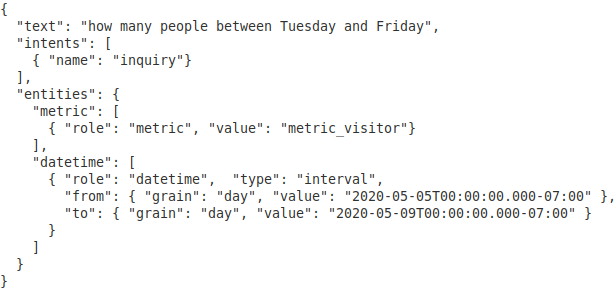
\includegraphics[width=\linewidth]{images/part4/chapter_nl_interfaces/message_intents.png}}
    \caption{Пример формализованного смысла сообщения}
    \label{fig:message_intents}
\end{figure}

При этом для представления результатов промежуточных этапов обработки используются иные форматы, модули которые их реализуют не имеют какой-либо единой основы и взаимодействуют посредством специализированных программных интерфейсов между ними, что приводит к несовместимости способов представления результатов на различных этапах обработки и конечного результата обработки текстов. Данная несовместимость в свою очередь ведет к существенным накладным расходам при разработке такой системы и в особенности при ее модификации.

В качестве решения проблемы совместимости предлагается использование подхода к обработке естественного языка на основе его формальной модели в виде набора онтологий, сформированных с использованием универсальных средств представления знаний, что будет способствовать интероперабельности как компонента по обработке естественного языка в целом с другими компонентами системы, так и между составляющими самого данного компонента.

Целью главы является формирование модели интерфейса, в основе которой лежит подход к обработке естественного языка на основе онтологий, содержащих формальное описание естественного языка.

\section{Предметная область и онтология естественно-языковых интерфейсов ostis-систем}

\textit{Естественно-языковой интерфейс} -- SILK-интерфейс (Speech – речь, Image – образ, Language – язык, Knowledge – знание), обмен информацией между компьютерной системой и пользователем в котором происходит за счёт диалога. Диалог ведётся на одном из естественных языков.

\begin{SCn}

    \scnheader{естественно-языковой интерфейс}
    \scnsuperset{речевой интерфейс}

\end{SCn}

\textit{Речевой интерфейс} -- SILK-интерфейс, обмен информацией в котором происходит за счёт диалога, в процессе которого компьютерная система и пользователь общаются с помощью речи. Данный вид интерфейса наиболее приближен к естественному общению между людьми.

В предлагаемом подходе можно выделить следующие этапы обработки естественного языка:
\begin{textitemize}
    \item лексический анализ;
    \item синтаксический анализ;
    \item понимание сообщения.
\end{textitemize}

В свою очередь, лексический анализ в включает в себя декомпозицию текста на токены и их сопоставление с лексемами.

Понимание сообщения сводится к генерации вариантов значения сообщения и выбору из них корректного на основании контекста, а также погружение его в данный контекст.

Ниже приведена структура решателя задач естественно-языкового интерфейса.

\begin{SCn}

    \scnheader{Решатель задач естественно-языкового интерфейса}
    \begin{scnrelfromset}{декомпозиция абстрактного sc-агента}
        \scnitem{Абстрактный sc-агент лексического анализа}
        \begin{scnindent}
            \begin{scnrelfromset}{декомпозиция абстрактного sc-агента}
                \scnitem{Абстрактный sc-агент декомпозиции текста на токены}
                \scnitem{Абстрактный sc-агент сопоставления токенов с лексемами}
            \end{scnrelfromset}
        \end{scnindent}
        \scnitem{Абстрактный sc-агент синтаксического анализа}
        \scnitem{Абстрактный sc-агент понимания сообщения}
    \end{scnrelfromset}

\end{SCn}

В свою очередь, \textit{Абстрактный sc-агент понимания сообщения} декомпозируется на:

\begin{SCn}

    \scnheader{Агент понимания сообщения}
    \begin{scnrelfromset}{декомпозиция абстрактного sc-агента}
        \scnitem{Абстрактный sc-агент генерации вариантов значения сообщения}
        \scnitem{Абстрактный sc-агент выбора и обновления контекста}
        \begin{scnindent}
            \begin{scnrelfromset}{декомпозиция абстрактного sc-агента}
                \scnitem{Абстрактный sc-агент разрешения контекста}
                \scnitem{Абстрактный sc-агент выбора смысла сообщения на основе контекста}
                \scnitem{Абстрактный sc-агент погружения сообщения в контекст}
            \end{scnrelfromset}
        \end{scnindent}
    \end{scnrelfromset}

\end{SCn}

Для каждого агента в базе знаний должна находиться спецификация, пример фрагмента такой спецификации приведен на рисунке \textit{\nameref{fig:agent_spec}}.

\begin{figure}[h]
    \centering
    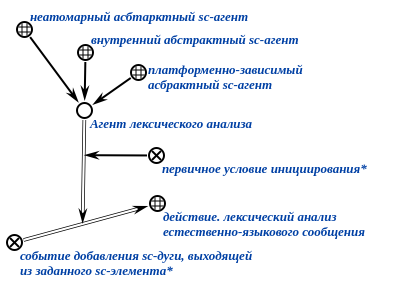
\includegraphics[width=0.4\textwidth]{images/part4/chapter_nl_interfaces/agent_spec.png}
    \caption{Пример спецификации агента.}
    \label{fig:agent_spec}
\end{figure}

\section{Предметная область и онтология лексического анализа естественно-языковых сообщений, входящих в ostis-систему}

\begin{SCn}

    \scnheader{действие. лексический анализ естественно-языкового сообщения}
    \begin{scnrelfromset}{обобщенная декомпозиция}
        \scnitem{действие. декомпозиция текста на токены}
        \scnitem{действие. сопоставление токенов с лексемами}
    \end{scnrelfromset}

\end{SCn}

С точки зрения ostis-системы, любой естественно-языковой текст является \textit{файлом} (т.е. SC-узлом с содержимым).

Этап лексического анализа представляет собой декомпозицию текста на последовательность токенов и сопоставление лексем с получившимися при данной декомпозиции токенами. Следует отметить, что данные токены при необходимости могут сопоставляться не с лексемами, а с их подмножествами, входящими в ее морфологическую парадигму, соответствующими определенным грамматическим категориям: падежу, числу, роду и т.д.

Результат лексического анализа представлен на рисунке \textit{\nameref{fig:lexical_result}}.

\begin{figure}[h]
    \centering
    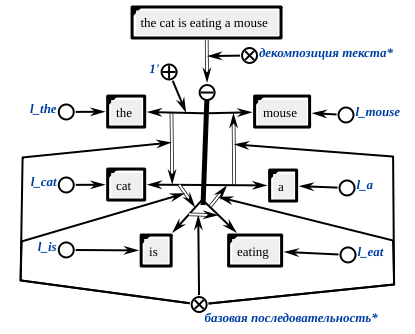
\includegraphics[width=0.4\textwidth]{images/part4/chapter_nl_interfaces/lexical.png}
    \caption{Пример результата лексического анализа.}
    \label{fig:lexical_result}
\end{figure}

Для осуществления лексического анализа, в базе знаний системы также должен присутствовать словарь, содержащий лексемы и их различные формы.

Под лексемой понимается единица словарного состава языка, которая представляет собой множество всех форм некоторого слова.
Пример спецификации лексемы в базе знаний приведен на рисунке \textit{\nameref{fig:lexeme_example}}.

\begin{figure}[h]
    \centering
    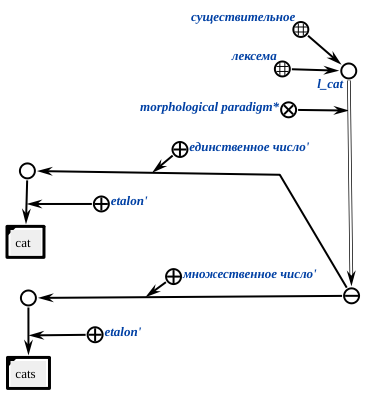
\includegraphics[width=0.4\textwidth]{images/part4/chapter_nl_interfaces/lexeme_example.png}
    \caption{Пример спецификации лексемы в базе знаний.}
    \label{fig:lexeme_example}
\end{figure}

\section{Предметная область и онтология синтаксического анализа естественно-языковых сообщений, входящих в ostis-систему}

Агент синтаксического анализа выполняет переход от размеченного на лексемы текста к его синтаксической структуре.
При этом из-за невозможности разрешения структурной неоднозначности на этапе синтаксического анализа, его результатом в общем случае будет являться множество потенциальных синтаксических структур.

Пример одной синтаксической структуры представлен на рисунке \textit{\nameref{fig:syntactic_result}}.

\begin{figure*}[h]
    \centering
    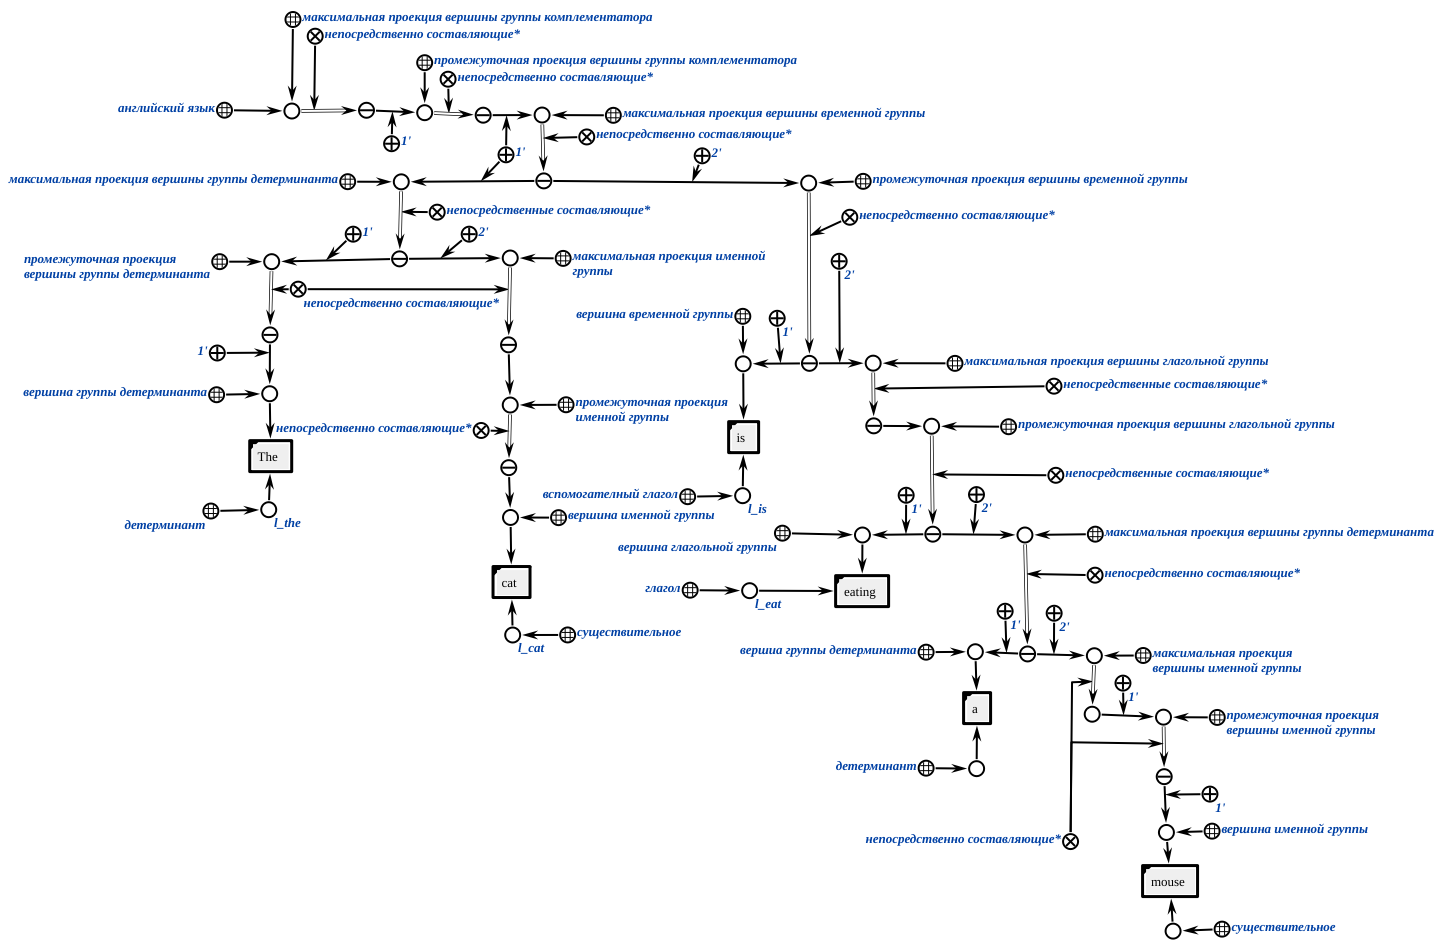
\includegraphics[width=\textwidth]{images/part4/chapter_nl_interfaces/syntactic.png}
    \caption{Пример синтаксической структуры.}
    \label{fig:syntactic_result}
\end{figure*}


\section{Предметная область и онтология понимания естественно-языковых сообщений, входящих в ostis-систему}

\begin{SCn}

    \scnheader{действие. понимание естественно-языкового сообщения}
    \begin{scnrelfromset}{обобщенная декомпозиция}
        \scnitem{действие. генерация вариантов значения сообщения}
        \scnitem{действие. выбор и обновление контекста}
        \begin{scnindent}
            \begin{scnrelfromset}{обобщенная декомпозиция}
                \scnitem{действие. разрешение контекста}
                \scnitem{действие. выбор смысла сообщения на основе контекста}
                \scnitem{действие. погружение сообщения в контекст}
            \end{scnrelfromset}
        \end{scnindent}
    \end{scnrelfromset}

\end{SCn}

\textit{Действие. генерация вариантов значения сообщения} -- действие, в ходе которого осуществляется формирование строгой дизъюнкции потенциально эквивалентных структур.

\textit{Потенциально эквивалентная структура*} -- бинарное ориентированное отношение, связывающее структуру и множество структур, которые потенциально могут быть эквивалентны ей, однако для достоверного определения факта требуются дополнительные действия.

При этом, переход от результата синтаксического анализа к потенциально эквивалентным сообщению структурам осуществляется по правилам, содержащихся в предметной области денотационной семантики. Пример одного из правил представлен на рисунке \textit{\nameref{fig:transition_to_semanic_rule}}.

\begin{figure*}[h]
    \centering
    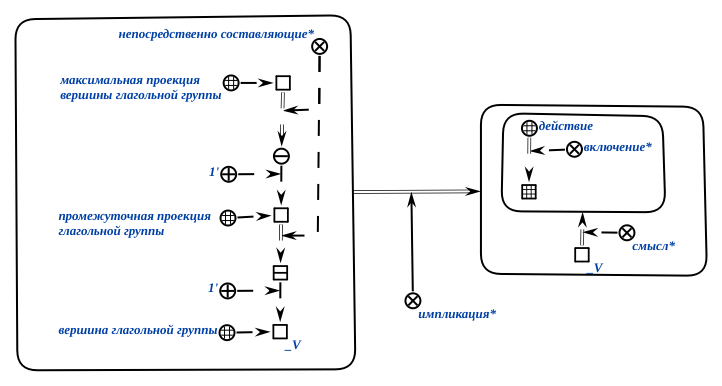
\includegraphics[width=0.7\textwidth]{images/part4/chapter_nl_interfaces/d_sem_3.png}
    \caption{Пример правила перехода от синтаксической структуры к семантике.}
    \label{fig:transition_to_semanic_rule}
\end{figure*}

В результате данного действия в базе знаний формируется структура, описывающая возможные варианты смысла сообщения, пример такой структуры в терминах грамматики составляющих\scncite{X_bar_syntax} приведен на \textit{\nameref{fig:messsage_meaning_variants}}. Наличие нескольких таких структур объясняется тем, что в общем случае на этапе синтаксического анализа выполняется генерация нескольких вариантов синтаксической структуры. Выбор корректного значения сообщения будет осуществлен в ходе выполнения последующих действий.

\begin{figure}[h]
    \centering
    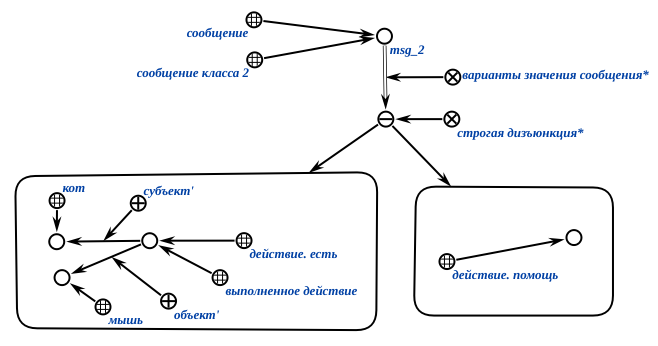
\includegraphics[width=0.45\textwidth]{images/part4/chapter_nl_interfaces/messsage_meaning_variants.png}
    \caption{Пример конструкции, описывающей потенциальные смыслы сообщения.}
    \label{fig:messsage_meaning_variants}
\end{figure}

Следует отметить, что при необходимости смысл сообщения может быть сгенерирован не только на основании его синтаксической структуры в терминах грамматики составляющих, но и других знаний о данном сообщении, например выделенных из текста данного сообщения троек вида субъект-отношение-объект, результата его классификации и т. п.

Дальнейшие этапы процесса понимания сообщения выполняются на основе контекста.

\textit{Контекст} - sc-структура, содержащая знания, которыми оперирует система в ходе одного или нескольких диалогов.
В общем случае, данные знания включают в себя как предварительно занесенные в БЗ, так и полученные в ходе работы с сенсоров и/или диалога.

\begin{SCn}

    \scnheader{контекст диалога}
    \scnsubset{контекст}
    \scnrelfrom{subdividing}{\scnkeyword{Типология контекстов диалога по глобальности\scnsupergroupsign}}
    \begin{scnindent}
        \begin{scneqtoset}
            \scnitem{тематический контекст}
            \scnitem{пользовательский контекст}
            \scnitem{глобальный контекст}
        \end{scneqtoset}
    \end{scnindent}

\end{SCn}

\textit{Тематический контекст} -- контекст диалога, содержащий специфические для темы сведения (сведения, полученные во время ведения диалога, на определенную тематику, например, при диалоге об определенном наборе сущностей).

\textit{Множество тематических контекстов диалога*} -- бинарное ориентированное отношение, диалог с ориентированным множеством его тематических контекстов.

\textit{Пользовательский контекст} -- контекст диалога, содержащие специфические для пользователя сведения, которые могут быть использованы в диалоге с ним на любую тематику. В общем случае пользовательский контекст имеет пересечение с согласованной частью БЗ (предварительно занесенная в БЗ достоверная информация о пользователе, прошедшая необходимую модерацию), но не включается в нее целиком (часть, полученная в ходе диалога в которой мы не уверены).
Пример соотнесения различных типов контекстов с согласованной частью базы знаний приведен на рисунке \textit{\nameref{fig:context_in_KB}}.

\textit{Глобальный контекст} -- контекст диалога, содержащий сведения, которые могут быть необходимы при ведении диалога с любым пользователем. Глобальный контекст -- подмножество согласованной части БЗ, содержащее те сведения, что допустимо использовать в диалоге. Например, в диалоге с определенным пользователем не нужно использовать:
\begin{itemize}
    \item находящуюся в базе знаний служебную информацию, необходимую для работы системы, но не предназначенную для использования в диалоге;
    \item части пользовательских контекстов иных пользователей.
\end{itemize}

\begin{figure}[h]
    \centering
    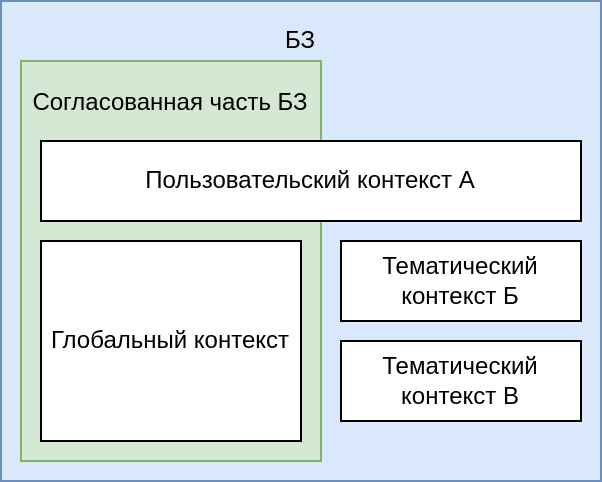
\includegraphics[width=0.4\textwidth]{images/part4/chapter_nl_interfaces/context_in_KB.png}
    \caption{Соотношение контекстов с согласованной частью баз знаний.}
    \label{fig:context_in_KB}
\end{figure}

\begin{SCn}

    \scnheader{контекст диалога}
    \scnrelfrom{subdividing}{\scnkeyword{Типология контекство по сроку достоверности знаний\scnsupergroupsign}}
    \begin{scnindent}
        \begin{scneqtoset}
            \scnitem{неизменяемый в ходе работы системы контекст диалога}
            \scnitem{изменяемый в ходе работы системы контекст диалога}
        \end{scneqtoset}
    \end{scnindent}

\end{SCn}

\textit{Неизменяемый в ходе работы системы контекст диалога} содержит в себе знания, необходимые для обеспечения выполнения системой своих функций,  которые были заложены в нее априорно ее разработчиками и/или администраторами и не изменяются в ходе ее функционирования на постоянной основе.

\textit{Изменяемый в ходе работы системы контекст диалога} содержит в себе знания, необходимые для обеспечения выполнения системой своих функций,  которые были ей получены в ходе ее работы и/или достоверность которых скоротечна.

\begin{SCn}


    \scnheader{изменяемый в ходе работы системы контекст диалога}
    \scnrelfrom{subdividing}{\scnkeyword{Типология изменяемых в ходе работы системы контекстов по источнику знаний\scnsupergroupsign}}
    \begin{scnindent}
        \begin{scneqtoset}
            \scnitem{контекст диалога, содержащий знания из внешних источников}
            \scnitem{контекст диалога, содержащий знания, полученные в ходе диалога}
        \end{scneqtoset}
    \end{scnindent}
    \scnrelfrom{subdividing}{\scnkeyword{Типология изменяемых контекстов по степени их достоверности\scnsupergroupsign}}
    \begin{scnindent}
        \begin{scneqtoset}
            \scnitem{достоверный контекст диалога}
            \scnitem{недостоверный контекст диалога}
        \end{scneqtoset}
    \end{scnindent}

\end{SCn}

Подмножество контекста может включаться в согласованную часть БЗ, например, если речь идет о каких-то предварительно занесенных в БЗ биографических сведениях -- дате рождения и т. п.

В каждый момент времени с пользователем связан 1 пользовательский диалоговый контекст (содержащий, по крайней мере известные заранее факты о нем: имя, возраст и т. п.) и несколько тематических.
Пример спецификации контекстов представлен на рисунке \textit{\nameref{fig:user_context}}.

\begin{figure}[h]
    \centering
    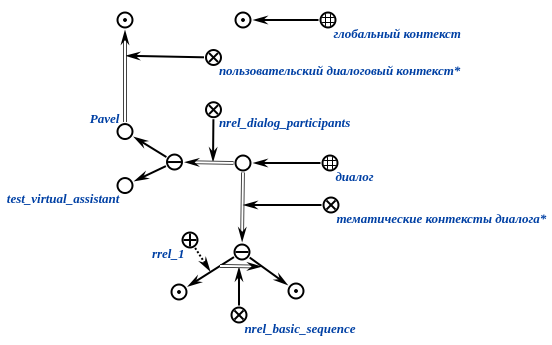
\includegraphics[width=0.5\textwidth]{images/part4/chapter_nl_interfaces/user_context.png}
    \caption{Пример спецификации контекстов.}
    \label{fig:user_context}
\end{figure}

Так, \textbf{действие. разрешение контекста} сводится к сопоставлению каждому варианту его значения соответствующего контекста.
Выбор производится на основании значения функции $F_{CTD}(T, C)$, где T - вариант трансляции, C - тематический контекст.
Подходящим контекстом для варианта трансляции считается тот, для которого значение этой функции максимально.
В случае, если подходящий контекст не найден, генерируется новый.
Пример результата данного действия представлен на рисунке \textit{\nameref{fig:relevant_contexts}}.

\begin{figure}[h]
    \centering
    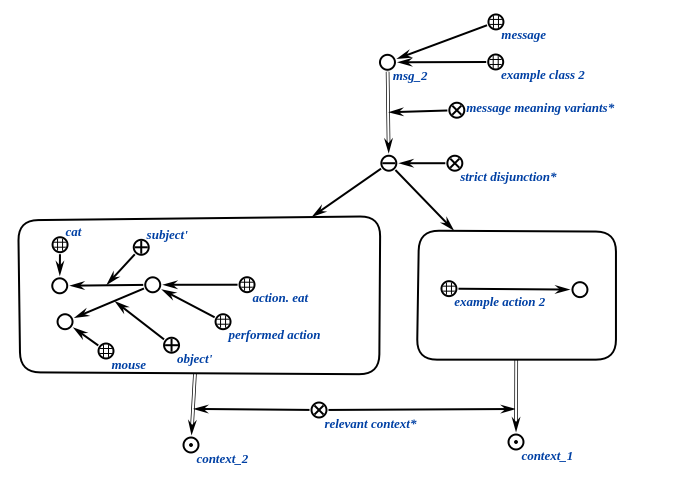
\includegraphics[width=0.45\textwidth]{images/part4/chapter_nl_interfaces/relevant_contexts.png}
    \caption{Пример сообщения, всем вариантам значения которого сопоставлен контекст.}
    \label{fig:relevant_contexts}
\end{figure}

\textbf{Действие. выбор смысла сообщения} представляет собой выбор из множества вариантов трансляции и соответствующих им контекстов одной пары и обозначение ее как эквивалентной сообщению конструкции. В простейшем случае, на данном этапе допустимо выполнить выбор в соответствии с рассчитанными на предыдущем этапе для пар потенциально эквивалентных структур и соответствующих им контекстов значениями функции $F_{CTD}(T, C)$ и выбрать пару, для которой оно максимально, однако при необходимости также возможно введение и отдельной функции.
Пример результата данного действия представлен на рисунке \textit{\nameref{fig:message_equivalent_structure}}.

\begin{figure}[h]
    \centering
    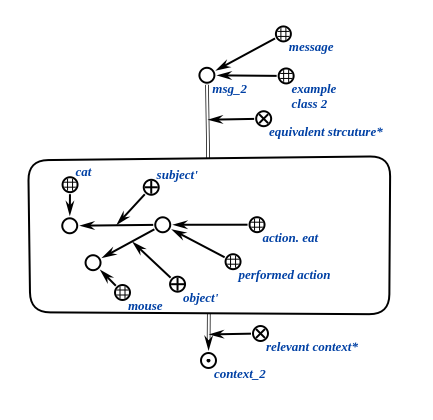
\includegraphics[width=0.35\textwidth]{images/part4/chapter_nl_interfaces/message_equivalent_structure.png}
    \caption{Пример конструкции, описывающей эквивалентную сообщению структуру.}
    \label{fig:message_equivalent_structure}
\end{figure}

\textbf{Действие. погружение сообщения в контекст} представляет собой погружение полученного смысла сообщения в контекст.
Кроме выбранного смысла сообщения, в контекст может добавляться и иная необходимая для обработки сообщения информация.
Кроме того, на данном этапе на основе хранящихся в контексте сведений также должно выполняться разрешение местоимений.
Примеры контекста до погружения в него сообщения и после погружения представлены на рисунках \textit{\nameref{fig:context_before_update}} и \textit{\nameref{fig:updated_context}}.

\begin{figure}[h]
    \centering
    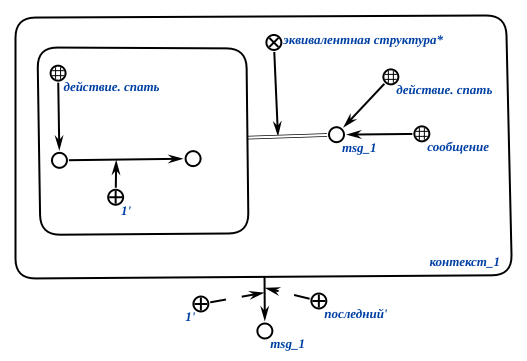
\includegraphics[width=0.4\textwidth]{images/part4/chapter_nl_interfaces/context_1.png}
    \caption{Пример контекста до погружения сообщения.}
    \label{fig:context_before_update}
\end{figure}

\begin{figure*}[h]
    \centering
    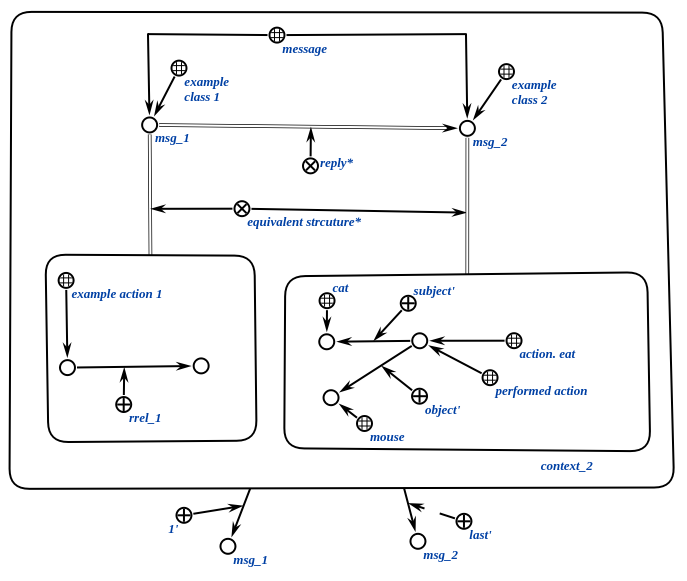
\includegraphics[width=0.7\textwidth]{images/part4/chapter_nl_interfaces/context_2.png}
    \caption{Пример контекста после погружения сообщения.}
    \label{fig:updated_context}
\end{figure*}

Таким образом, актуальная информация собирается в тематический контекст, объединив который с контекстом пользователя и глобальным контекстом можно получить общий контекст, на основании которого должны осуществляться требуемые действия системы, включая генерацию ответа системы.

%Под вопросом
\section{Предметная область и онтология синтеза естественно-языковых сообщений ostis-системы}
\section{Модели, методы и средства адаптации пользовательских интерфейсов к носителям китайского языка}
\label{section_chinese_interfaces}
Данный раздел посвящен рассмотрению разработки естественно-языковых интерфейсов интеллектуальных систем, ориентированных на решение задач преобразования текстов естественного языка в фрагменты базы знаний, и задач генерации текстов естественного языка из фрагментов базы знаний. Предложена семантическая модель естественно-языковых интерфейсов, которая включает в себя модель базы знаний лингвистики, а также модель решателей задач для решения данных двух задач в естественно-языковых интерфейсах, что позволяет проводить объединение лингвистических знаний на различных уровнях по обработке естественного языка в единую базу знаний, а также глубокую интеграцию различных моделей решения задач для обработки естественного языка. Описание принципов разработки китайско-языкового интерфейса осуществляется на основе предложенной единой модели естественно-языковых интерфейсов.

В настоящее время интерфейсы на основе распознавания текстов естественного языка, являются наиболее распространенными компонентами любых поисковых систем (например, Google, Yandex, Baidu и другие) или вопросно-ответных систем на основе базы знаний (см. \scncite{Wu2019}). В отличие от речевых интерфейсов, данные интерфейсы, как правило, ориентированы на обработку текстов естественного языка. В обычных современных поисковых системах вопросно-ответные системы начали разрабатываться как их подсистемы, ориентированные на обработку вопросительных предложений (или декларативных предложений).

Модульная схема (рисунок \textit{\nameref{fig:schema-natural-interface}})современных вопросно-ответных систем, основанных на знаниях описывает общий автоматизированный процесс информационного взаимодействия между текстами естественного языка (особенно вопросительными предложениями), предоставляемыми человеческими пользователями и базами знаний интеллектуальных систем.

\begin{figure}[H]
	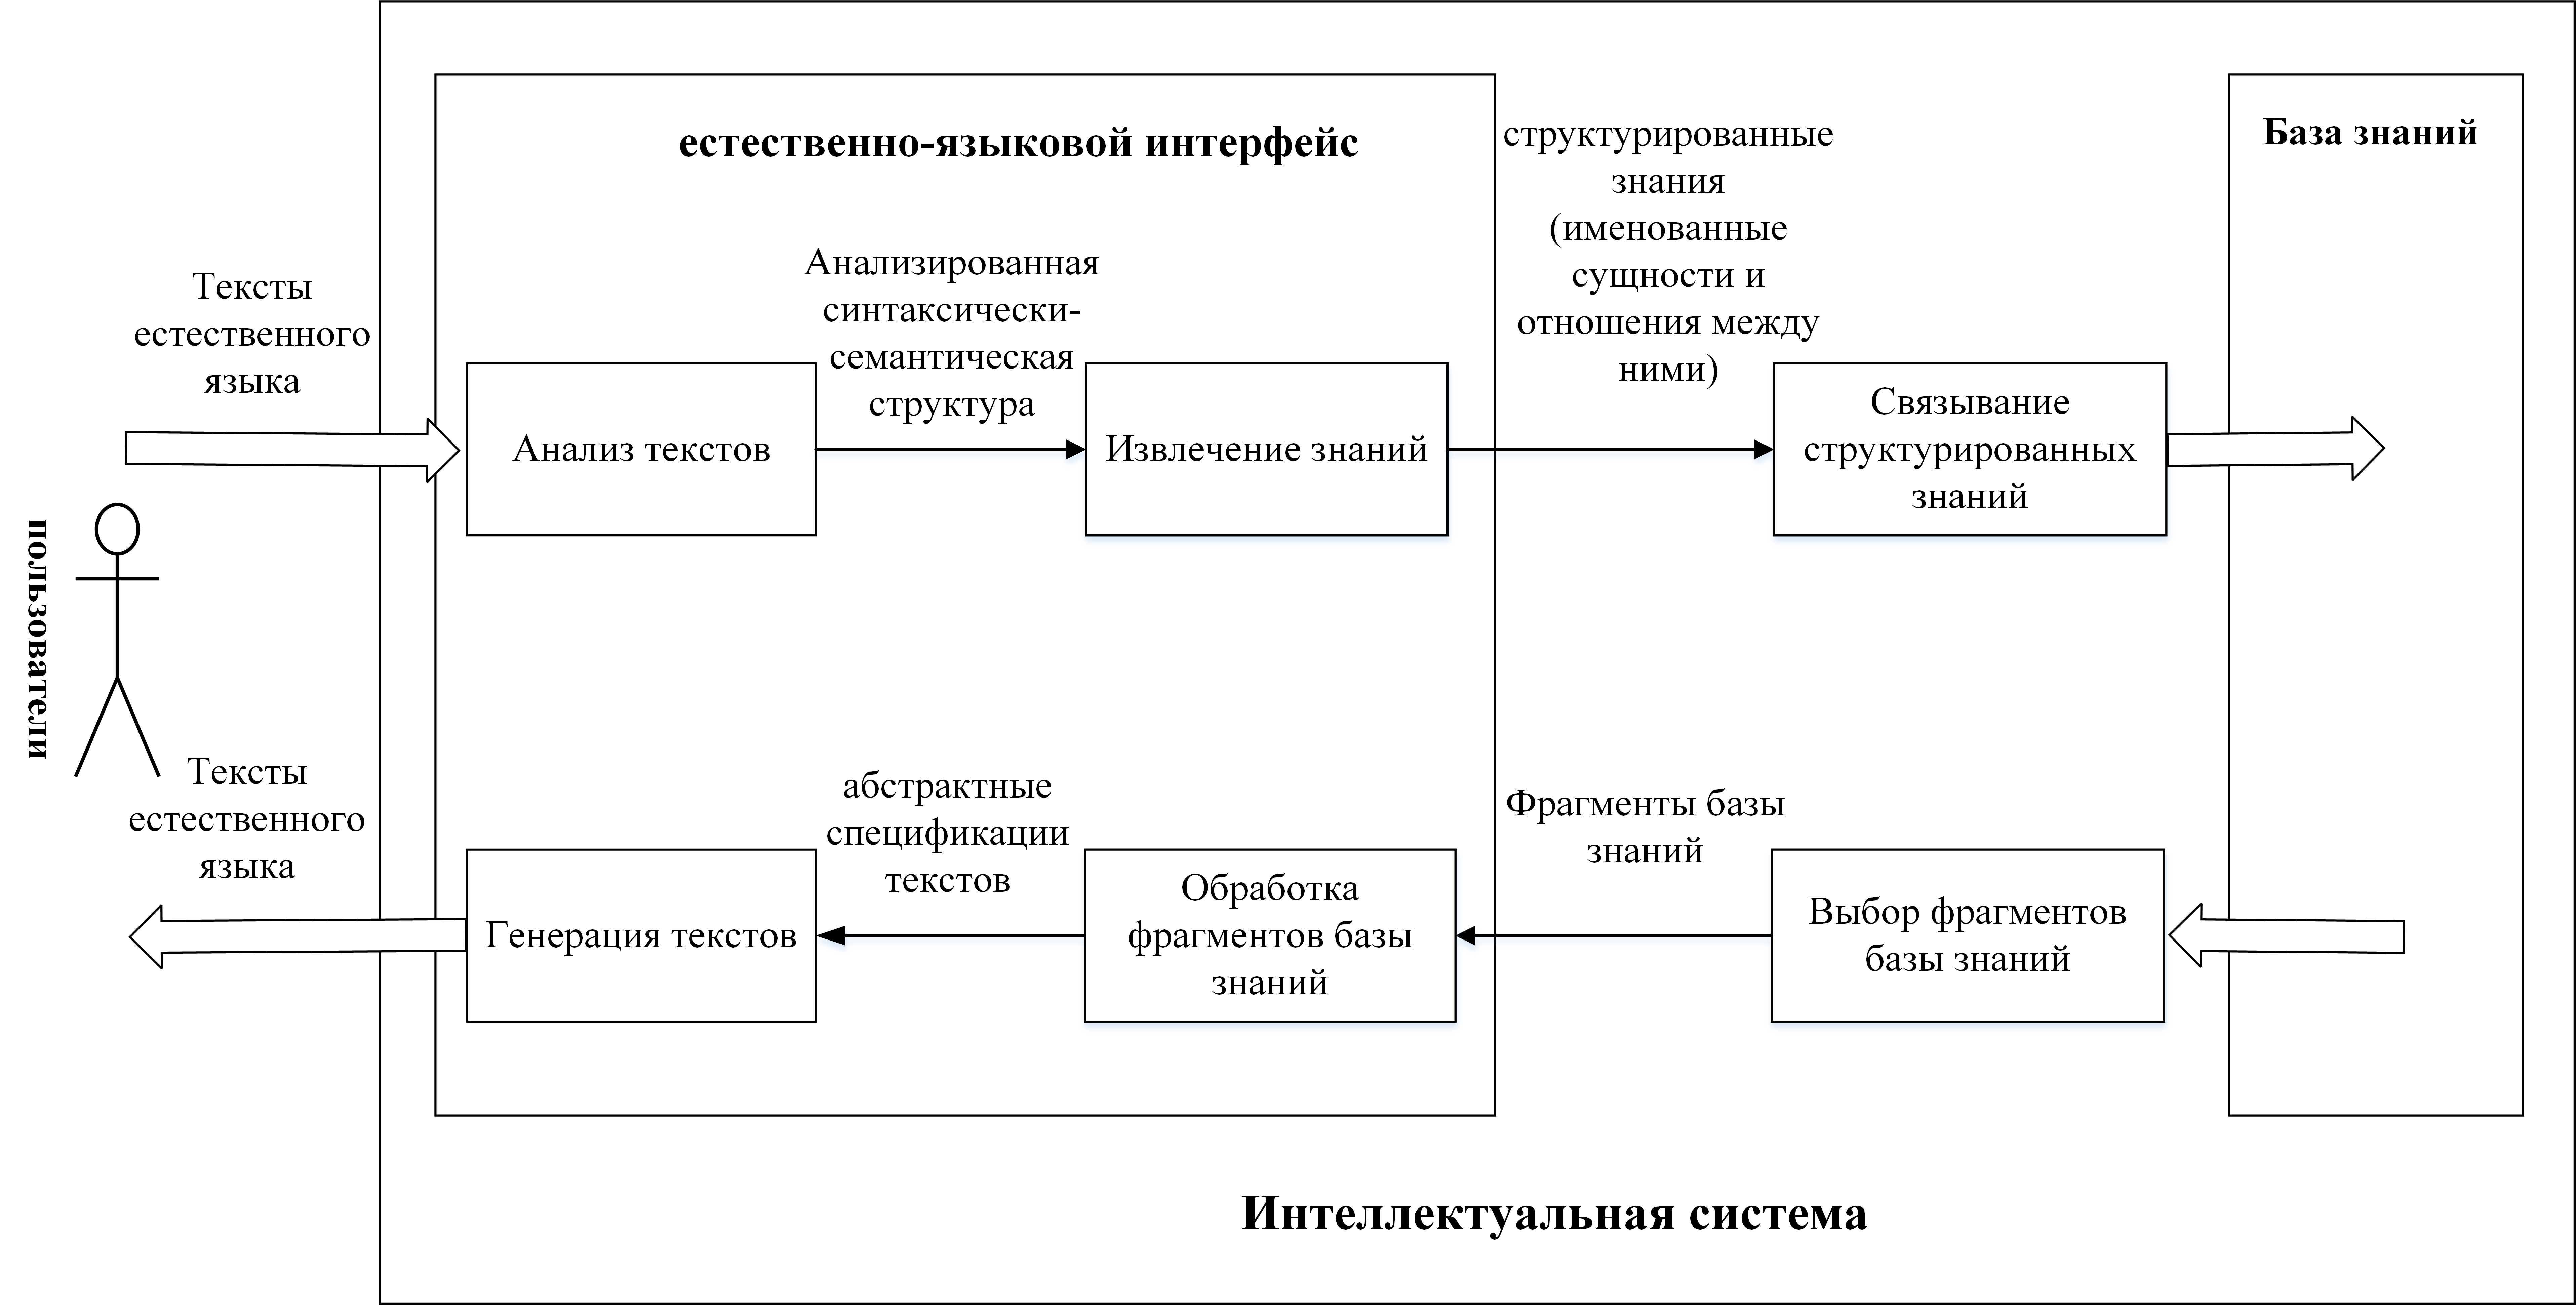
\includegraphics[scale=0.8,width=1.0\textwidth]{images/part4/chapter_chinese/schema1.png}
	\caption{Модульная схема вопросно-ответных систем, основанных на знаниях}
	\label{fig:schema-natural-interface}
\end{figure}

Современные вопросно-ответные системы в основном сосредоточены на обработке вопросительных предложений и поиске правильных ответов в базе знаний систем. Кроме того, генерация ответов вопросно-ответных системах часто напрямую выводит правильный фрагменты базы знаний в качестве ответов, которые неудобны для чтения пользователями. Генерация ответов может быть легко реализована в современных вопросно-ответных системах. В большинстве систем даже нет необходимости реализовывать  модули обработки фрагментов базы знаний и генерации текстов.

В нашей работе разработка естественно-языковых интерфейсов интеллектуальных систем ориентирована на решение следующих двух задач:
\begin{textitemize}
	\item преобразование входных текстов естественного языка (в частности
	повествовательные предложения) в фрагменты базы знаний интеллектуальных систем (приобретение/извлечение фактографических знаний (в основном именованных сущностей и отношений между ними));
	\item генерация текстов естественного языка (в частности
	повествовательные предложения) из фрагментов базы знаний интеллектуальных систем (генерация текстов естественного языка).
\end{textitemize}

Разработка естественно-языковых интерфейсов для современных интеллектуальных систем, основанных на знаниях, в общем случае требует рассмотрения следующих двух основных аспектов:
\begin{textitemize}
	\item типы обрабатываемого естественного языка, т. е. характеристики различных типов естественного языка;
	\item диапазон базы знаний интеллектуальных систем, т. е. широта знаний в базах знаний интеллектуальных систем.
\end{textitemize}

По статистике лингвистов, в мире существуют тысячи естественных языков. Однако в Интернете существуют лишь десятки естественных языков, которые широко используются конечными пользователями для общения, например, русский язык, английский язык, китайский язык и т. д. Каждый естественный язык имеет свои уникальные особенности. Таким образом, при использовании моделей, методики и средств для обработки текстов различных естественных языков необходимо учитывать соответствующие характеристики различных естественных языков. Кроме того, диапазон базы знаний также влияет на сложность разработки естественно-языковых интерфейсов. Например, базы знаний всемирного масштаба (см. \scncite{Liu2020}, см. \scncite{Abu2020}), в которых источники знаний ориентированы на Интернет, т. е. в базах знаний интеллектуальных систем хранятся знания здравого смысла (англ. commonsense knowledge). А базы знаний специализированные (см. \scncite{Xu2016}), в которых источники знаний ориентированы на различные энциклопедии (например, автомобильная энциклопедия, энциклопедия о фильмах, энциклопедия о разных дисциплинах (дискретная математика, история и другие) и т.д.), т. е. в базах знаний интеллектуальных систем хранятся конкретные отраслевые знания (т. е. знания об ограниченной предметной области). Общие базы знаний обращают внимание на широту хранимых знаний, подчеркивают интеграцию больше количества именованных сущностей по различным предметным областям и отношений между ними. Таким образом, общие базы знаний не обеспечивают высокую точность хранимых в них знаний (см. \scncite{Liu2020}). А также огромное количество именованных сущностей и отношений между ними в базе знаний приводит к высокой сложности поиска и обработки фрагментов базы знаний. В отличие от общих баз знаний, в специализированных базах знаний уделяется больше внимания глубине и точности хранящихся знаний, удовлетворяющих решение различных задач в интеллектуальных системах с низкой сложностью. 

В соответствии с двумя перечисленными выше аспектами, естественно-языковые интерфейсы интеллектуальных систем можно разделить на следующие формы:
\begin{textitemize}
	\item \textbf{интерфейс, не зависящий от конкретного естественного языка и конкретной предметной области.} В данном случае это означает, что интерфейс может обрабатывать тексты любых видов естественных языков, например, русский язык, арабский язык, английский язык и китайский язык и так далее, а также обрабатывать любую сложную структуру знаний, т. е. знания в базах знаний всемирного масштаба;
	\item интерфейс, зависящий от конкретного естественного языка, но не зависящий от конкретной предметной области. В этом случае интерфейс может анализировать только тексты определенного естественного языка и обрабатывать любую сложную структуру знаний;
	\item \textbf{интерфейс, не зависящий от конкретного естественного языка, но зависящий от конкретной предметной области.} В этом случае интерфейс может анализировать тексты любых видов естественных языков, обрабатывать тексты естественного языка, описывающие факты в конкретной предметной области. И специализированная база знаний является основой базы знаний данной интеллектуальной системы. Следует отметить, что описание фактов в разных предметных областях может использовать особенные виды предложений. Таким образом, обработка текстов естественного языка, описывающих факты в разных предметных областях (например, исторический текст, юридический текст, текст в дисциплинах), имеет разную степень сложности;
	\item \textbf{интерфейс, зависящий от конкретного естественного языка и зависящий от конкретной предметной области.} Данный интерфейс считается самым основным естественно-языковым интерфейсом в интеллектуальных системах. В этом случае интерфейсу нужно только анализировать тексты определенного естественного языка и обрабатывать легкую структуру знаний в специализированной базе знаний. 	
\end{textitemize}

Всем известно, что построение базы знаний всемирного масштаба является огромном проектом. А также база знаний всемирного масштаба в основном используется в Интернет ориентированных поисках, рекомендациях и вопросно-ответных задачах. Сценарий применения относительно единственно. Однако плотность знаний в специализированной базе знаний более высока, \textbf{интерфейс, не зависящий от конкретного естественного языка, но зависящий от конкретной предметной области} могут выполняться больше сценарии применения. 

В современных интеллектуальных системах отсутствует единая основа для разработки естественно-языковых интерфейсов, которая приводит к высокой сложности и трудоемкости разработки естественно-языковых интерфейсов. Как приобретение фактографических знаний, так и генерация текстов естественного языка считаются подзадачами обработки естественного языка. С точки зрения интеллектуальных систем, данные подзадачи представляют собой разновидности так называемых комплексных задач, решение которых до сих пор является актуальной темой исследований в области искусственного интеллекта. В целом, решение данных подзадач требует сочетание различных типов лингвистических знаний и интеграция различных моделей решения задач по обработке естественного языка. Однако в разработке естественно-языковых интерфейсов отсутствует единый принцип для интеграции различных типов лингвистических знаний и моделей решения задач для обработки естественного языка.

На данный момент существует большое количество методов для приобретения фактографических знаний и генерации текстов естественного языка, которые в основном можно разделить на два направления:
\begin{textitemize}
	\item методы на основе правил и лингвистических знаний;
	\item методы машинного обучения, основанные на математической статистике и теории информации.
\end{textitemize}

Первое направление предполагает разработку систем на основе лингвистических правил, соответствующих грамматике определенного естественного языка, сформулированных вычислительными лингвистами и другими лингвистами. В данных системах могут строиться правила извлечения, шаблоны для генерации текстов и другие на основе лингвистических знаниях для извлечения фактографических знаний и генерации текстов. 

Под извлечением фактографических знаний понимается приобретение фактографической информации, такой как понятия, именованные сущности, отношения между ними, а также определенный тип событий из текстов естественного языка, причем извлеченные результаты формализуются в виде внутреннего языка представления знаний интеллектуальных систем (например, RDF и другие). По сути, с точки зрения построения базы знаний интеллектуальных систем, отношения между именованными сущностями рассматриваются как особенные сущности, которые извлекаются из текстов естественного языка. 

Задача извлечения фактографических знаний из текстов естественного языка можно разделить на два направления по сфере извлеченной области:
\begin{textitemize}
	\item извлечение фактографических знаний из закрытых областей;
	\item извлечение фактографических знаний из открытых областей.
\end{textitemize}

Задача извлечения фактографических знаний из закрытых областей часто требует заранее определенных типов именованных сущностей и отношений между ними. Однако в области извлечения фактографических знаний может быть не существуют ограниченные и определенные типы именованных сущностей и отношений между ними. Таким образом, цель извлечения фактографических знаний из открытой области состоит в том, чтобы извлекать различные наборы именованных сущностей и отношений между ними из массивных и разнородных корпусов текстов естественного языка без требований заранее заданного словаря для определения типа данных именованных сущностей и отношений между ними.

Извлечение фактографических знаний из открытых областей напрямую определяет относительные слова или словосочетания в текстах, анализируя тексты естественного языка (в частности, предложения), чтобы реализовать моделирование классификаций именованных сущностей и отношений между ними без необходимости заранее определений категорий данных именованных сущностей и отношений между ними.  Например, система CORE (см. \scncite{Tseng2014}) использует ряд технологий обработки китайского языка, таких как сегментация слов, автоматическая морфологическая разметка (POS tagging), скорректированная и подходящая для текстов китайского языка, синтаксический анализ, семантический анализ и правила извлечения для извлечения именованных сущностей и отношений между ними из текстов китайского языка. В данных системах построение правил вручную неэффективно, а также построенные правила сложно переносятся в других интеллектуальных системах для обработки китайского языка.

Для генерации текстов естественного языка существует классическая конвейерная архитектура (см. \scncite{Gatt2017}), на основе которой большинство систем генерации текстов имеет три основных модуля:
\begin{textitemize}
	\item планирование содержания текстов: уточнение, какая информация из входных данных будет включена в сгенерированные тексты, и как она будет организована;
	\item микро-планирование: решение, каким образом выбранная информация будет реализована языковыми средствами в виде предложений на естественном языке. В этом процессе преобразования информации в лингвистические выражения, обычно представлены предложения в виде структур семантических и/или синтаксических отношений;
	\item реализация на естественном языке: производство грамматически правильных предложений естественного языка.
\end{textitemize}

В самом начале системы генерации текстов широко используют шаблоны и грамматические правила, построенные исследователями для генерации текстов естественного языка. Система NaturalOWL (см. \scncite{Androutsopoulos2013}) представляет собой классическую систему генерации естественного языка, которая рационально применяет шаблоны и лингвистические правила для генерации текстов естественного языка (в основном английский язык), описывающих фрагменты OWL онтологий. Однако, в данной системе не предоставлена модель семантического представления знаний, что позволяет представлять различные виды знаний в единой базе знаний, включая лингвистические знания, логический вывод на онтологиях лингвистики и шаблоны, построенные на онтологиях. 

Второе направление, широко применяемое в настоящее время в современных интеллектуальных системах, предполагает использование различных моделей машинного обучения, основанных на математической статистике и теории информации, которые направлены на моделирование текстов естественного языка.

В настоящее время подходы, основанные на моделей машинного обучения (в частности модели нейронных сетей), в основном используются для извлечения фактографических знаний из закрытых областей, например, серия моделей предварительной подготовки BERT (см. \scncite{Devlin2018}), GPT (см. \scncite{Brown2020}) и т.д. Использование моделей нейронных сетей всегда требует дорогие аппаратные оборудования и очень больших корпусов данных, которые аннотируются вручную человеком. Более того, производительность данных моделей сильно зависит от качества аннотирования обучающих выборок. 

Для обучения моделей нейронных сетей, ориентированных на генерацию текстов естественного языка, обучающие данные обычно представляются в виде пары входов (фрагменты базы знаний) и выходов (тексты естественного языка) (см. \scncite{Moryossef2019}). В последние годы в проекте WebNLG (см. \scncite{Gardent2017}) основная задача направлена на разработку нейронных генераторов с помощью моделей нейронных сетей для решения задач генерации текстов. Для разработки нейронных генераторов команда проекта предоставляет обучающие данные, которые состоят из пар Данные/Тексты для английского языка и русского языка, где данные представляют собой фрагменты базы знаний в виде RDF, извлеченных из DBpedia (см. \scncite{Lehmann2015}). Для других естественных языков, таких как китайский язык, наборы данных для обучения генераторов отсутствуют, хотя и существуют несколько известных баз знаний на китайском языке в области обработки китайского языка, например, CN-DBpedia (см. \scncite{Xu2017}), zhishi.me (см. \scncite{Niu2011}) и другие, которые могут предоставлять фрагменты базы знаний в виде RDF. Построение высококачественных наборов данных для китайского языка является трудоемким и трудно-затратным процессом. 

Разработанные системы извлечения фактографических знаний из открытых областей и разработанные различные генераторы были успешно применены в различных областях. Тем не менее, к проблемам существующих решений к разработке естественно-языкового интерфейса и обработке естественного языка в естественно-языковом интерфейсе можно отнести:
\begin{textitemize}
	\item отсутствие единой основы в процессе разработки естественно-языковых интерфейсов и интеграция различных компонентов (база знаний по обработке естественного языка, компонент для извлечения фактографических знаний, компонент для генерации текстов), разработанных разными разработчиками, приводит к сложной трудоемкости и невозможности распараллеливания разработки естественно-языковых интерфейсов;
	\item отсутствие возможности использования единой основы для представления различных видов лингвистических знаний в единой базе знаний для обработки естественного языка;
	\item отсутствие подходов к возможности интеграции различных моделей решения задач для извлечения фактографических знаний и генерации текстов естественного языка;
	\item для приобретения фактографических знаний в существующих онтологических подходах построенные правила часто применимы только в извлечениях фактографических знаний из закрытых областей и ограниченных условиях;
	\item качество извлеченных фактографических знаний и генерируемых текстов зависит от искусственно сконструированных шаблонов и правил, но построение конкретных шаблонов и правил для текстов различных естественных языков является чрезвычайно сложной и трудоемкой задачей из-за отсутствия единой основы;
	\item для приобретения фактографических знаний и генерации текстов, большие языковые модели на основе моделей нейронных сетей используется для обработки естественного языка. Используя модели нейронных сетей, необходимо дорогие аппаратные оборудования и высококачественные согласованные учебные корпусы, которые  крайне сложно получить и построить.
\end{textitemize}

Построение единой семантической модели естественно-языковых интерфейсов осуществляется на основе \scnkeyword{Технологии OSTIS} (см. \scncite{Golenkov2014a}), что обеспечивает единую основу для эффективного объединения различных лингвистических знаний, включая правила извлечения, шаблоны для генерации текстов и другие лингвистические знания по обработке естественного языка, а также глубокой интеграции различных моделей решения задач (например логические модели на основе правил, модели нейронных сетей и другие) для решения задач преобразования текстов естественного языка в фрагменты базы знаний и генерации текстов естественного языка из фрагментов базы знаний в естественно-языковых интерфейсах (рисунок \textit{\nameref{fig:structure-sc-model-natural-interface}}). Системы, построенные по указанной Технологии OSTIS, названы ostis-системами.

\begin{figure}[H]
	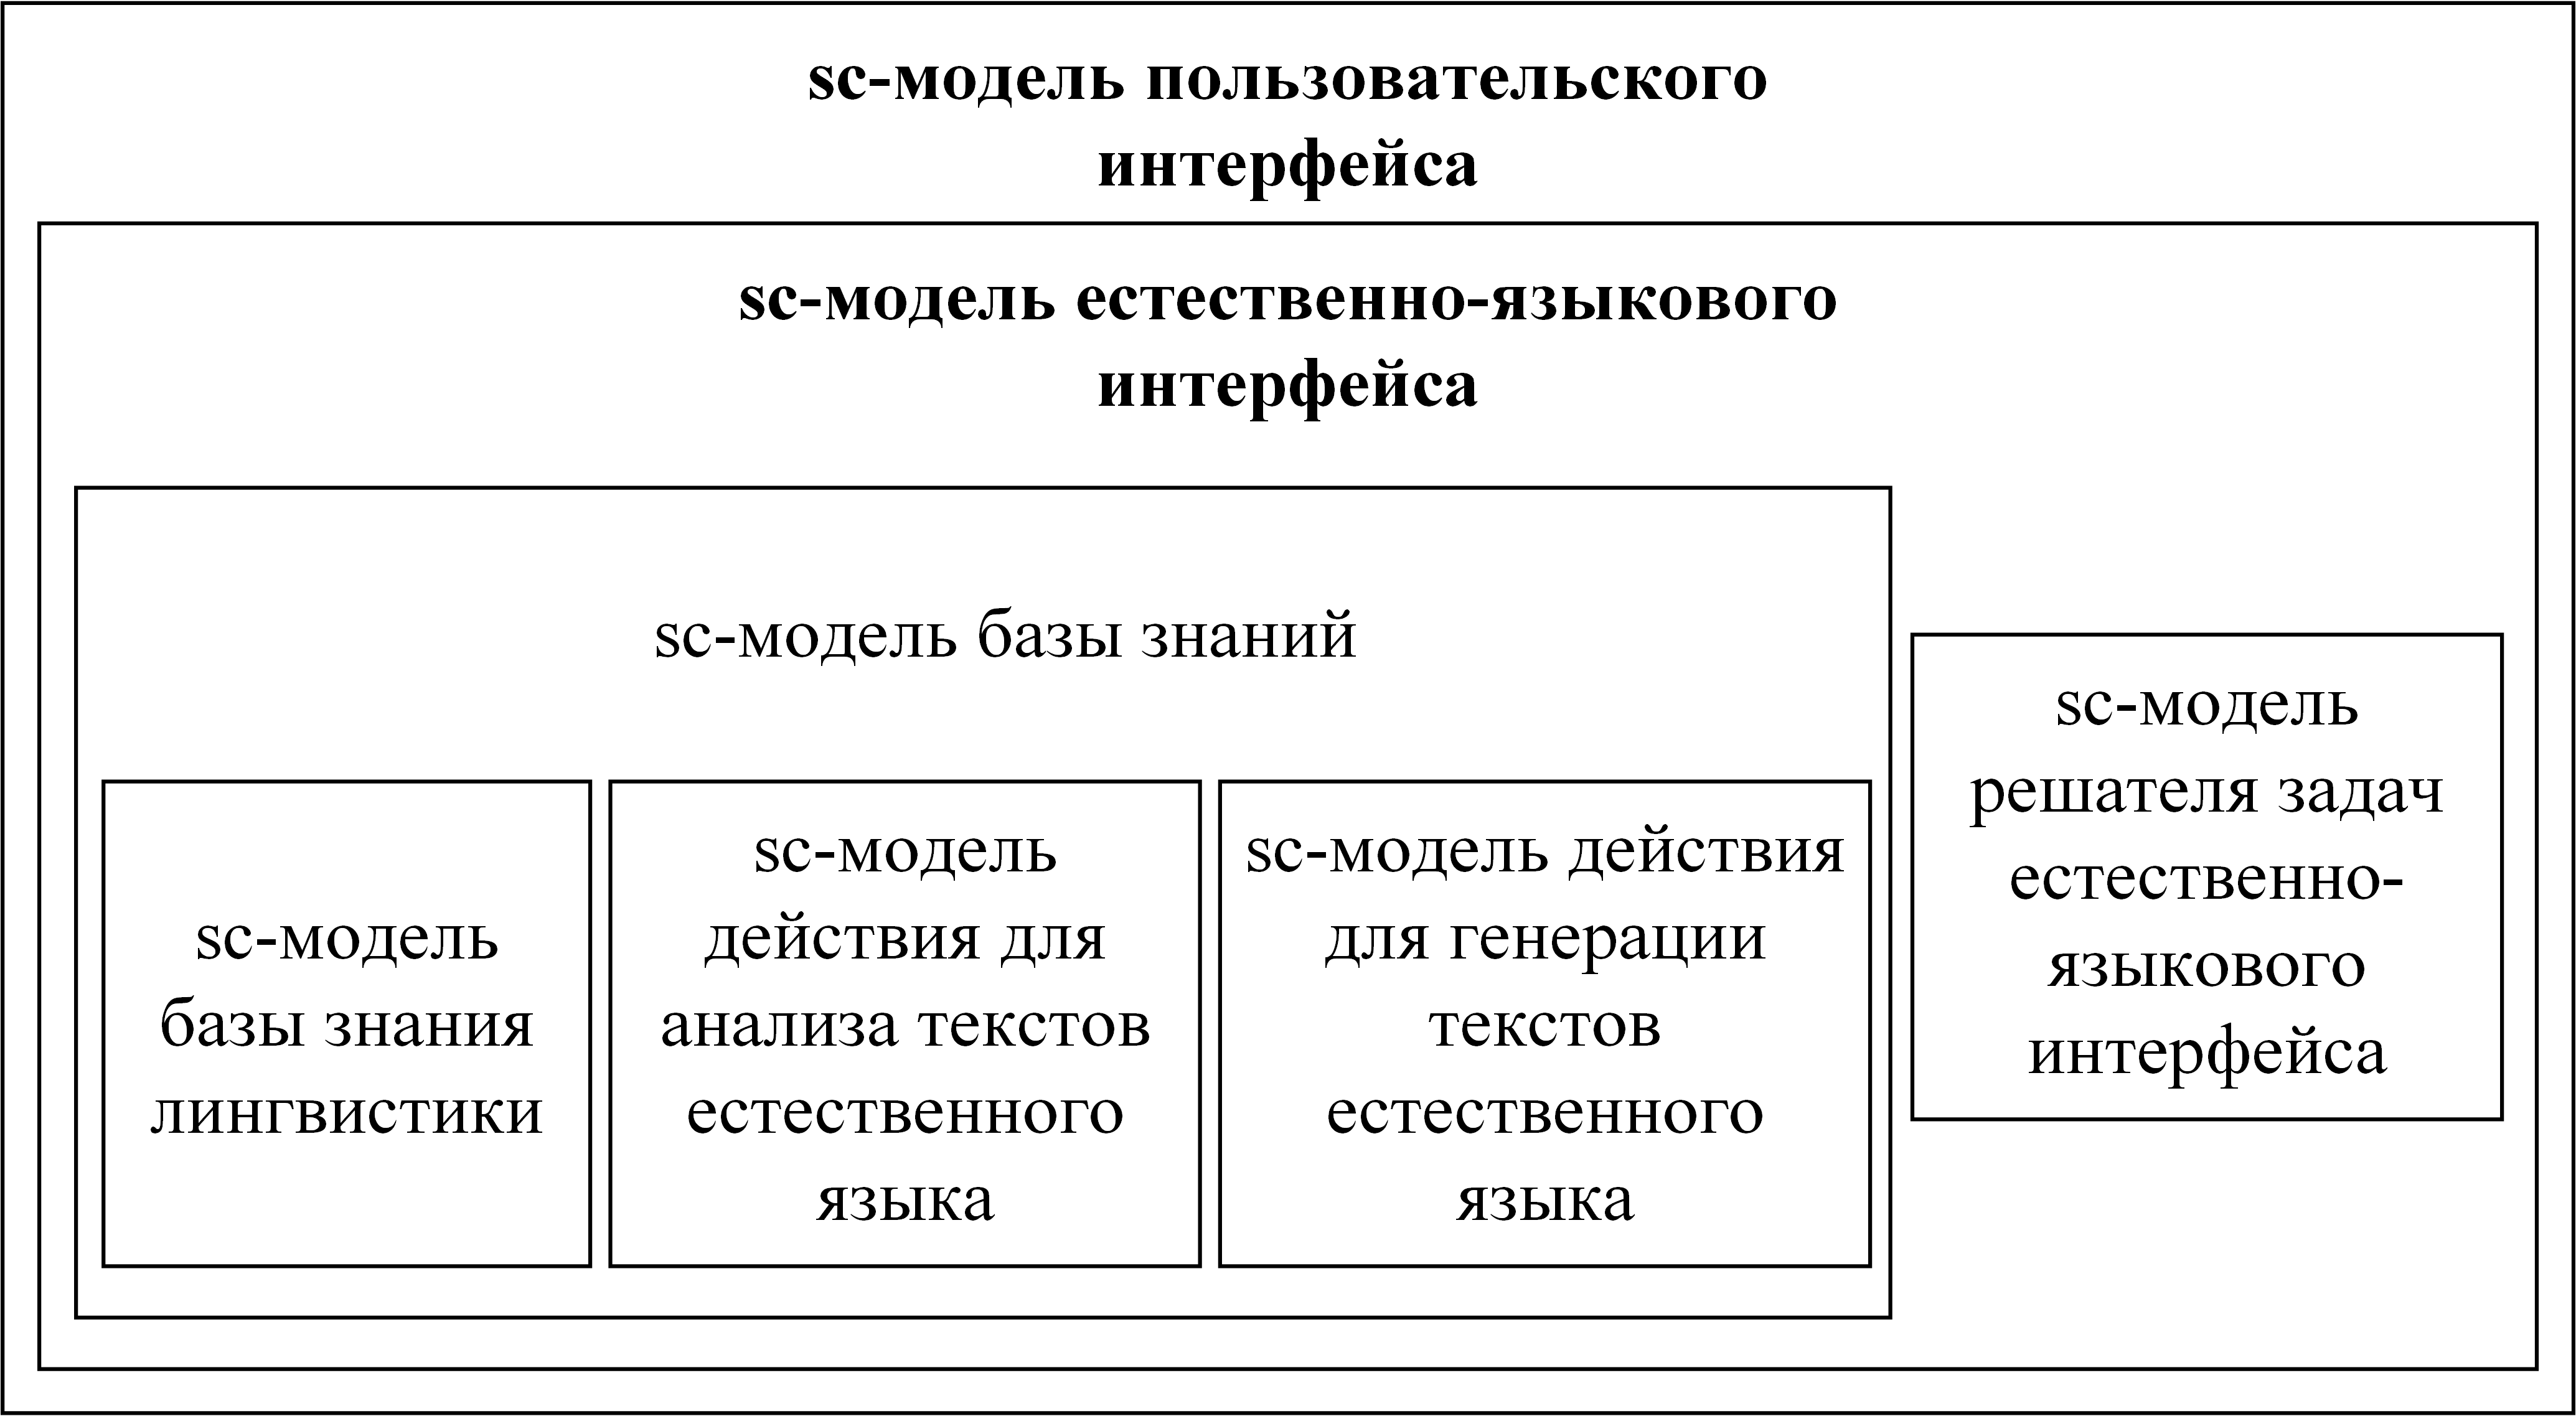
\includegraphics[scale=0.8,width=1.0\textwidth]{images/part4/chapter_chinese/structure_interface.png}
	\caption{Общая структура sc-модели естественно-языковых интерфейсов ostis-систем}
	\label{fig:structure-sc-model-natural-interface}
\end{figure}

Единая семантическая модель естественно-языковых интерфейсов интеллектуальных систем по конкретной предметной области позволяет, в принципе, потенциально реализовать преобразование текстов различных естественных языков в фрагменты базы знаний и генерации текстов различных естественных языков из фрагментов базы знаний, просто сложность построения базы знаний по обработке конкретного естественного языка, объединяющей различные виды лингвистических знаний, будет разным в зависимости от особенностей конкретного естественного языка, а также потребуются определенные дополнительные sc-агенты, входящие в решатели задач естественно-языкового интерфейса по особенностям конкретного естественного языка, интегрирующие логические модели на основе правил и модели нейронных сетей для обработки текстов конкретного естественного языка.

\subsection{SC-модель базы знаний лингвистики}
База знаний лингвистики содержит формальное описание необходимых лингвистических знаний для анализа текстов естественного языка и генерации текстов естественного языка (см. \scncite{Qian2020}). Соответствующие онтологии обеспечивают формальное описание понятий, используемых для представления таких лингвистических знаний на различных уровнях от базовых слов до синтаксических или семантических структур текстов естественного языка по обработке естественного языка. Лингвистические теории, предложенные лингвистами, обеспечивают теоретическую основу для построения SC-модели базы знаний лингвистики. 

В рамках \scnkeyword{Технологии OSTIS} sc-модель базы знаний рассматривается, как иерархическая система выделенных предметных областей и соответствующих им онтологий (см. \scncite{Davydenko2018}). Основная иерархия SC-модели базы знаний лингвистики, используемая для решения задач преобразований текстов естественного языка в фрагменты базы знаний и генерации текстов естественного языка из фрагментов базы знаний:
\begin{SCn}
	\scnheader{SC-модель базы знаний лингвистики}
	\scnidtf{SC-модель лингвистической базы знаний}
	\scnidtf{SC-модель базы знаний по обработки естественного языка}
	\scnidtf{SC-модель базы знаний естественно-языковых интерфейсов}
	\begin{scnrelfromset}{декомпозиция раздела}
		\scnitem {Предметная область лексического анализа}
		\scnitem {Предметная область синтаксического анализа}
		\scnitem {Предметная область семантического анализа}
	\end{scnrelfromset}
\end{SCn}

Предметная область лексического анализа включает в себя ряд онтологий для лексического анализа, которые описывают характеристики слов и синтаксические функции слов, части речи и т.д. В обработке естественного языка \textit{слово} -- это наименьшая единица естественного языка, несущая семантику, которая служит для наименования объектов, их качеств, характеристик и взаимодействий, а также для служебных целей. \textit{Номинативная единица} -- устойчивая последовательность комбинаторных вариантов лексем.
\begin{SCn}
	\scnheader{текст естественного языка}
	\scnsubset{файл}
	\scnheader{слово}
	\scnsubset{файл}
	\scnheader{номинативная единица}
	\scnsubset{файл}
\end{SCn} 

В русском, английском или других европейских языках структура слова изучается в рамках морфологии. Лексема рассматривается для описания особенностей слов в европейских языках, обладающих признаком морфологической парадигмы. В китайском языке из-за письменной традиции (текст китайского языка состоит потока иероглифов без естественных пробелов), единица сегментации рассматривается как наименьшая единица для обработки текстов китайского языка, был предложен в государственном стандарте «Стандарт сегментации слов современного китайского языка, используемый для обработки информации». 
\begin{SCn}
	\scnheader{единица сегментации}
	\scnidtfdef{базовая единица для обработки китайского языка с определенными семантическими или грамматическими функциями}
	\scnsubset{файл}
\end{SCn}

Стоит отметить, что описание единица сегментации ориентировано на компьютерную обработку китайского языка и не полностью совпадает с описанием слов в китайской лингвистике.

\textit{Часть речи} -- это категория слов естественного языка, определяемая морфологическими, синтаксическими и семантическими особенностями. Хотя часть речи, предложенная для анализа текстов европейских языков, не полностью подходит к анализу текстов китайского языка, но часть речи может частично решить задачи в обработке китайского языка. В 2001 г. был предложен государственный стандарт «Принцип частеречной разметки
в обработке современной китайской информации», устанавливающий конкретный стандарт морфологической разметки. 
\begin{SCn}
	\scnheader{часть речи по обработке китайского языка}
	\scnrelto{семейство подмножеств}{единица сегментации}
	\scnhaselement{существительное}
	\scnhaselement{прилагателбное}
	\scnhaselement{глагол}
	\scnhaselement{наречие}
	\scnhaselement{идиома}
	\scnhaselement{союз}
	\scnhaselement{географическое название}
	\scnhaselement{модальный глагол}
\end{SCn}

Категории в части речи по обработке китайского языка построены с учета особенности китайского языка на лингвистических теорий европейских языков. 

Предметная область синтаксического анализа описывает характеристики синтаксиса естественного языка, функциональные характеристики синтаксических компонентов (таких как, слово, словосочетание, предложение и т.д.). Среди них в области обработки естественного языка предложение всегда рассматривается как наименьшая единица исследования. Анализ предложений является важным промежуточным этапом, связывающим анализ всех текстов и анализ отдельных слов. 

В зависимости от особенностей китайского языка существуют соответствующие различные синтаксические структуры для предложений китайского языка.

\begin{SCn}
	\scnheader{предложение китайского языка}
	\begin{scnrelfromset}{разбиение}
		\scnitem{простое предложение}
		\scnidtfdef{предложение содержит в себе одну предикативную единицу}
		\scnitem{сложное предложение}
		\scnidtfdef{предложение содержит в себе больше одну предикативную единицу}
	\end{scnrelfromset}
\end{SCn}

\begin{SCn}
	\scnheader{предложение китайского языка}
	\begin{scnrelfromset}{разбиение}
		\scnitem{предложение с подлежащим и сказуемым}
		\scnitem{предложение без подлежащего и сказуемого}
		\scnitem{предложение с особенным знаком алфавита синтаксиса}
	\end{scnrelfromset}
\end{SCn}

\begin{SCn}
	\scnheader{член предложения\scnrolesign}
	\begin{scnrelfromset}{разбиение}
		\scnitem{главный член предложения\scnrolesign}
		\begin{scnindent}
			\begin{scnrelfromset}{разбиение}
				\scnitem{подлежащее\scnrolesign}
				\scnitem{сказуемое\scnrolesign}
				\scnitem{прямое дополнение\scnrolesign}
			\end{scnrelfromset}
		\end{scnindent}
		\scnitem{второстепенный член предложения\scnrolesign} 
		\begin{scnindent}
			\begin{scnrelfromset}{разбиение}
				\scnitem{косвенное дополнение\scnrolesign}
				\scnitem{определение\scnrolesign}
				\scnitem{обстоятельство\scnrolesign}
			\end{scnrelfromset}
		\end{scnindent}
	\end{scnrelfromset}
\end{SCn}

\textit{Член предложения\scnrolesign} -- рольное отношение, связывающее декомпозицию текста с файлом, содержимое которого (отдельное слово или словосочетание из текста) играет в делительном тексте определенную синтаксическую роль (см. \scncite{Hardzei2022}).

\begin{SCn}
	\scnheader{отношение зависимости*}
	\scnidtfdef{описание зависимости отдельных слов или словосочетаний в предложении друг от друга.}
	\scnhaselement{суъбект*}
	\scnhaselement{объект*}
	\scnhaselement{дополнение глагола*}
	\scnhaselement{определитель*}
	\scnhaselement{атрибут*}
	\scnhaselement{модификатор*}
\end{SCn}

На основе теории синтаксиса грамматики зависимостей для китайского языка, \textit{отношение зависимости*} -- отношение, связывающее делительные два файла из предложения естественного языка направленными связями, содержимое которых отдельно называется исходным словом (англ. head), которое часто играет роль сказуемое' в предложении, и целевым словом (англ. depedent). Каждое целевое слово несет синтаксическую функцию по зависимости к исходному слову. В общем случае, при синтаксическом анализе предложений китайского языка глаголы (или глагольные словосочетания) (также называется конечные глаголы, исходные слова) часто считаются структурными центрами придаточной структуры. Все остальные синтаксические единицы (слова или словосочетания) прямо или косвенно связаны с глаголом посредством направленных связей (т. е. направление с глаголом до других синтаксических единиц). В области обработки китайского языка были предложены Харбинским политехническим университетом ряды отношений зависимости (см. \scncite{Liu2006}).

В логической онтологии предметной области синтаксического анализа можно описать ряды логических определений и логических утверждений для обработки предложений. В виде логических утверждений могут быть построены правила или шаблоны для приобретения фактографических знаний и генерации текстов, которые могут использоваться решателями задач для решения конкретных задач в естественно-языковых интерфейсах.
\begin{figure}[H]
	\centering
	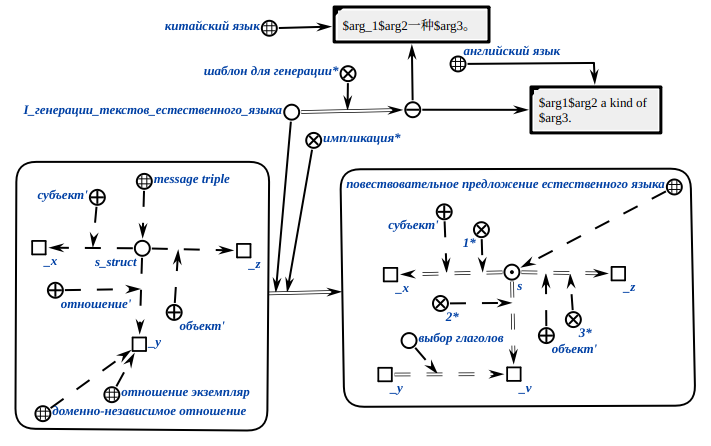
\includegraphics[scale=0.8]{images/part4/chapter_chinese/ruleGeneration.png}
	\caption{Логическое утверждение про генерации предложения на основе шаблона}
	\label{fig:template-generation}
\end{figure}

На рисунке \textit{\nameref{fig:template-generation}} указано на SCg-коде, что эвристическое правило, используемое для генерации текстов естественного языка. Как показано на рисунке, если определено, что отношение в ``message triple'' принадлежит к множеству предметно-независимых отношений, то шаблон используется для генерации текстов. Компоненты субъект и объект в ``message triple'' заполняются в параметр 1 и параметр 3 в шаблоне, соответственно, а затем соответствующий глагол (или глагольное словосочетание) для отношения в ``message triple'' выбирается в качестве параметра 2 в шаблоне. Понятия ``message triple'' и множества предметно-независимых отношений будут показаны ниже.

Предметная область семантического анализа описывает семантические характеристики слов и семантическую структуру предложений естественного языка, функциональные характеристики семантики компонентов (слов, словосочетаний и предложений и т.д.), семантические роли, правила семантического анализа и так далее.

Предметная область семантического анализа на уровне лексемы описывает семантические классификации общих базовых понятий, выраженных лексемой, или привязку лексемы к отдельным сущностям. Предметная область была построена на основе различных типов баз семантических знаний о естественном языке, используемых для семантического анализа на уровне лексемы или предложений, например, WordNet, ConcetpNet, The Semantic Knowledge base of Modern Chinese (см. \scncite{Wang2006}), TAPAZ-2 и т. д.

\begin{SCn}
	\scnheader{семантические категории в естественном языке}
	\scnhaselement{семантические категории для глаголов}
	\scnhaselement{семантические категории для существительных}
	\scnhaselement{семантические категории для прилагателбных}
	\scnhaselement{семантические категории для наречий}
\end{SCn}


\begin{SCn}
	\scnheader{участник воздействия*}
	\scnidtf{участник акции*}
	\scnidtf{участник события*}
	\scniselement{неролевое отношение}
	\scnrelfrom{первый домен}{индивид}
	\scnrelfrom{вторый домен}{акция}
	\begin{scnrelfromset}{разбиение}
		\scnitem {субъект*}
		\begin{scnindent}
			\begin{scnrelfromset}{разбиение}
				\scnitem {инициатор*}
				\scnitem {вдохновитель*}
				\scnitem {распространитель*}
				\scnitem {вершитель*}
			\end{scnrelfromset}
		\end{scnindent}
		\scnitem {объект*}
		\begin{scnindent}
			\begin{scnrelfromset}{разбиение}
				\scnitem {покрытие*}
				\scnitem {корпус*}
				\scnitem {прослойка*}
				\scnitem {сердцевина*}
			\end{scnrelfromset}
		\end{scnindent}
	\end{scnrelfromset}
\end{SCn}

\textit{Индивид} является разновидностью стереотипа как отдельной сущности, которая представляет собой  экземпляр конкретных понятий. 

\textit{Участник действия*} -- это неролевое отношение, которое связывает действие с индивидом, участвующим в нем, в определенной степени его можно рассматривать как семантическую роль действия. Соответственно действие обычно выражается глаголом или глагольной фразой в предложении.

В свою очередь, аналогично предметная область семантического анализа на уровне предложения описывает семантическую структуру предложений, семантические отношения между компонентами (словами, словосочетаниями и т.д.) в предложении, а также семантические отношения между предложениями в текстах. Некоторые открытые базы знаний, например, TAPAZ-2, PropBank и другие, послужили основой для построения данной предметной области.

В sc-модели естественно-языковых интерфейсов база знаний лингвистики просто предоставляет синтаксические лингвистические знания решателями задач для решения соответствующих задач в естественно-языковых интерфейсах. Кроме того, естественно-языковые интерфейсы должны иметь динамическую возможность выполнять некоторые действия для решения задач по обработке естественного языка в естественно-языковых интерфейсах. 
\begin{SCn}
	\scnheader{действие для естественно-языковых интерфейсов}
	\begin{scnrelfromset}{декомпозиция}
		\scnitem{действие для преобразования текстов естественного языка в фрагменты базы знаний}
		\scnitem{действие для генерации текстов естественного языка из фрагментов базы знаний}
	\end{scnrelfromset}
\end{SCn}

\begin{SCn}
	\scnheader{действие для преобразования текстов естественного языка в фрагменты базы знаний}
	\begin{scnrelfromset}{декомпозиция}
		\scnitem{действие для разбиения текстов на отдельные единицы}
		\scnitem{действие для разметки отдельных единиц}
		\scnitem{действие для синтаксического анализа}
		\scnitem{действие для семантического анализа}
		\scnitem{действие для формирования структур фактографических знаний}
		\scnitem{действие для связывания фактографических знаний в базу знаний}
		\scnitem{действие для определения противоречий}
		\scnitem{действие для устранения противоречий}
	\end{scnrelfromset}
\end{SCn}

\begin{SCn}
	\scnheader{действие для генерации текстов естественного языка из фрагментов базы знаний}
	\begin{scnrelfromset}{декомпозиция}
		\scnitem{действие для локализации фрагментов базы знаний}
		\scnitem{действие для преобразования фрагментов в стандартные базовые sc-конструкции}
		\scnitem{действие для определения проектных базовых sc-конструкций}
		\scnitem{действие для преобразования проектных sc-конструкций в message triple}
		\scnitem{действие для генерации результирующих текстов из message triple}
	\end{scnrelfromset}
\end{SCn}

С точки зрения генерации текста из фрагментов базы знаний ostis-системы, следует отметить, что ``message triple'' представляет собой вид упорядоченной последовательности текстов естественного языка, представленной в виде <субъект, отношение, объект>, где субъект -- это всегда идентификатор множества sc-узлов, обозначающих понятия, не являющиеся отношениями, или элемент данного множества sc-узлов; отношение -- идентификатор множества sc-узлов, обозначающих ролевые или неролевые отношения, которые указывает на связку, соединяющую субъект и объект; объект -- идентификатор множества sc-узлов, обозначающих понятия, не являющиеся отношениями, или элемент данного множества sc-узлов. У состава sc-структур (и sc-конструкций) есть sc-дуги, которые имеют конкретные значения. Таким образом, sc-структуры (и sc-конструкции) с sc-дугами нужны преобразовать в ``message triple'' в текстовом виде, которые легче представляют в виде текстов естественного языка.

В процессе генерации, ``message triple'' рассматривается как промежуточное преобразование между sc-структурой и результирующим текстом, главным образом потому что данный вид упорядоченной последовательности текстов легче выразить в виде текстов естественного языка (в основном предложения), используя либо модели шаблонов или правил, либо современные модели нейронных сетей. 

\subsection{SC-модель решателя задач естественно-языковых интерфейсов}
Для реализации естественно-языковых интерфейсов ostis-систем необходимо разработать SC-модель решателя задач естественно-языковых интерфейсов, в рамках которой SC-модель решателя задач рассматривается как иерархическая система агентов (см. \scncite{Shunkevich2017}), способного выполнять вышеупомянутые действия в sc-памяти для решения задач анализа текстов естественного языка и генерации текстов естественного языка в естественно-языковых интерфейсах.
\begin{SCn}
	\scnheader{SC-модель решателя задач естественно-языковых интерфейсов}
	\scnidtf{SC-модель решателя задач по обработке естественного языка}
	\begin{scnrelfromset}{декомпозиция}
		\scnitem{SC-модель решателя задач анализа текстов естественного языка}
		\scnitem{SC-модель решателя задач генерации текстов естественного языка}
	\end{scnrelfromset}
\end{SCn}

В естественно-языковых интерфейсах SC-модель решателя задач анализа текстов естественного языка предназначена для решения задач извлечения фактографических знаний (как правило, именованные сущности и отношения между ними) из текстов естественного языка в открытых областях.

\begin{SCn}
	\scnheader{SC-модель решателя задач анализа текстов естественного языка}
	\scnidtf{SC-модель решателя задач приобретения фактографических знаний}
	\begin{scnrelfromset}{декомпозиция абстрактного sc-агента}
		\scnitem{Абстрактный sc-агент лексического анализа}
		\begin{scnindent}
			\begin{scnrelfromset}{декомпозиция абстрактного sc-агента}
				\scnitem {Абстрактный sc-агент разбиения текстов на отдельные единицы}
				\scnitem {Абстрактный sc-агент разметки отдельных единиц}
			\end{scnrelfromset}
		\end{scnindent}
		\scnitem{Абстрактный sc-агент синтаксического анализа}
		\scnitem{Абстрактный sc-агент семантического анализа}
		\scnitem{Абстрактный sc-агент извлечения структур фактографических знаний в базу знаний}
		\begin{scnindent}
			\begin{scnrelfromset}{декомпозиция абстрактного sc-агента}
				\scnitem {Абстрактный sc-агент формирования структур фактографических знаний}
				\scnitem {Абстрактный sc-агент связывания фактографических знаний в базу знаний}
				\scnitem {Абстрактный sc-агент определения противоречий}
				\scnitem {Абстрактный sc-агент устранения противоречий}
			\end{scnrelfromset}
		\end{scnindent}
		\scnitem{Абстрактный sc-агент логического вывода}
	\end{scnrelfromset}
\end{SCn}

\textit{\textbf{Абстрактный sc-агент разбиения текстов на отдельные единицы}} -- группы агентов, реализующие механизмы декомпозиции входных текстов естественного языка на лексические единицы. Компоненты (слова, словосочетания, предложения и другие) входных текстов естественного языка могут быть определены по определенному стандарту конкретного естественного языка.

\textit{\textbf{Абстрактный sc-агент разметки отдельных единиц}} -- коллектив агентов, реализующих механизмы разметки раздельных лексических единиц по определенному принципу конкретного естественного языка, устанавливающему конкретный стандарт разметки. 

\textit{\textbf{Абстрактный sc-агент синтаксического анализа}} -- коллектив агентов, реализующих механизмы построения синтаксической структуры входных текстов естественного языка.

\textit{\textbf{Абстрактный sc-агент семантического анализа}} -- коллектив агентов, реализующих механизмы построения семантической структуры входных текстов естественного языка.

\textit{\textbf{Абстрактный sc-агент извлечения структур фактографических знаний в базу знаний}} -- коллектив агентов, реализующих механизмы интеграции структур фактографических знаний в базу знаний ostis-систем по конкретной предметной области.

\textit{\textbf{Абстрактный sc-агент формирования структур фактографических знаний}} -- коллектив агентов, реализующих механизмы, которые устанавливают структуры фактографических знаний во входных текстах естественного языка (т.е. определение именованных сущностей и отношений между ними).

\textit{\textbf{Абстрактный sc-агент связывания фактографических знаний в базу знаний}} -- коллектив агентов, реализующих механизмы связывания каждого элемента фактографических знаний в базу знаний ostis-систем по конкретной предметной области, включая наполнение экземпляров понятий с использованием именованных сущностей, сопоставление именованных сущностей и отношений между ними в базе знаний ostis-систем по конкретной предметной области.

В процессе отображения структур знаний в базу знаний, при сравнении структур знаний, извлеченных в результате анализа входных текстов естественного языка, с знаниями, хранящимися в базе знаний ostis-систем по конкретной предметной области, \textit{\textbf{Абстрактный sc-агент определения противоречий}} -- коллектив агентов, реализующих механизмы определения противоречий, например, для конкретной именованной сущности во входных текстах естественного языка может быть существует несколько соответствующих экземпляров понятий. 

\textit{\textbf{Абстрактный sc-агент устранения противоречий}} -- коллектив агентов, реализующих механизмы устранения противоречий, в случае обнаружения противоречий. 

\textit{\textbf{Абстрактный sc-агент логического вывода}} -- коллектив агентов, реализующих механизмы, которые используют логические правила, записанные средствами SC-кода, для синтаксического анализа, семантического анализа и также извлечения структур фактографических знаний. Таким образом, данный агент может взаимодействовать с агентами синтаксического, семантического анализа и агентом извлечения структур фактографических знаний.

При решении задач генерации текстов SC-модель решателя задач генерации текстов естественного языка разработана на основе классического конвейера. Хотя разработка SC-модели данного решателя основана на классическом конвейере, разработка конкретных составов решателя может быть гибка за счет использования многоагентного подхода (см. \scncite{Qian2022}). Для генерации текстов конкретного естественного языка, составы решателя задач можно соответствующим образом легко модифицировать.
\begin{SCn}
	\scnheader{SC-модель решателя задач генерации текстов естественного языка}
	\begin{scnrelfromset}{декомпозиция абстрактного sc-агента}
		\scnitem{Абстрактный sc-агент локализации фрагмента базы знаний}
		\scnitem{Абстрактный sc-агент планирования структуры текстов}
		\scnitem{Абстрактный sc-агент микро-планирования}
		\scnitem{Абстрактный sc-агент реализации текстов естественного языка}
	\end{scnrelfromset}
\end{SCn}

\begin{SCn}
	\scnheader{Абстрактный sc-агент локализации фрагмента базы знаний}
	\begin{scnrelfromset}{декомпозиция абстрактного sc-агента}
		\scnitem{Абстрактный sc-агент локализации sc-структуры в базе знаний}
		\scnitem{абстрактный sc-агент разделения конкретной sc-структуры на базовые стандартные sc-конструкции}
		\scnitem{Абстрактный sc-агент определения конкретных проектных sc-конструкций}
		\scnitem{Абстрактный sc-агент преобразования конкретных sc-конструкций в соответствующие им message triple}
	\end{scnrelfromset}
\end{SCn}

\textit{\textbf{Абстрактный sc-агент локализации sc-структуры в базе знаний}} -- группа агентов, предоставляющих поиск sc-структуры из базы знаний ostis-систем по конкретной предметной области, составляющего из sc-конструкций стандартного вида, из которых будем преобразовывать тексты естественного языка. С точки зрения генерации текстов, на этом этапе, по сути, определяется, о чем мы хотим поговорить. 

\textit{\textbf{Абстрактный sc-агент разделения конкретной sc-структуры на базовые стандартные sc-конструкции}} -- группа агентов, реализующих механизмы декомпозиции поисковой sc-структуры на базовые стандартные sc-конструкции, которые могут быть переведены в ``message triple''. 

В некоторых случаях разделенные базовые sc-конструкции из sc-структуры являются избыточными, т.е. не все разделенные базовые sc-конструкции нужно преобразовывать в ``message triple'', а затем в тексты естественного языка, а некоторые sc-конструкции не являются той информацией, которую ожидают пользователи. Таким образом, естественно-языковой интерфейс требует окончательного выбора некоторых среди разделенных sc-конструкций в качестве проектных sc-конструкций, предоставляющих максимально полезную информацию пользователям, и даже подходящую для пользователей (для разных пользователей нужно предоставлять сгенерированные тексты различных стилей, например, для специалистов нужно использовать специальные термины в сгенерированных текстах). 

\textit{\textbf{Абстрактный sc-агент определения конкретных проектных sc-конструкций}} -- группа агентов, реализующих механизмы определения подходящих конкретных sc-конструкций, предоставляющих информацию пользователям и возможно удовлетворяющих конкретных пользователей. 

\textit{\textbf{Абстрактный sc-агент преобразования конкретных sc-конструкций в соответствующие им message triple}} -- группа агентов, реализующих механизмы перевода выбранных конкретных sc-конструкций в соответствующие ``message triple''.

\textit{\textbf{Абстрактный sc-агент планирования структуры текстов}} -- группа агентов, реализующих функцию структурирования сгенерированных текстов, т.е. определения упорядоченности ``message triple'', в данной упорядоченности ``message triple'' будут представлены в сгенерированных текстах. 
\begin{SCn}
	\scnheader{Абстрактный sc-агент планирования структуры текстов}
	\begin{scnrelfromset}{декомпозиция абстрактного sc-агента}
		\scnitem{Абстрактный sc-агент упорядочения message triple}
		\scnitem{Абстрактный sc-агент упорядочения именованных сущностей в каждом message triple}
	\end{scnrelfromset}
\end{SCn}

В общем случае, в базе знаний ostis-систем в качестве идентификаторов sc-элементов чаще всего используются имена (термины) соответствующих сущностей, представленные отдельными словами или словосочетаниями на различных естественных языках, но также могут использоваться иероглифы на китайском языке. Таким образом, в качестве идентификаторов (названий, терминов) именованных сущностей в ``message triple'' можно прямо использовать в сгенерированных текстах естественного языка. 

\textit{\textbf{Абстрактный sc-агент микро-планирования}} -- группа агентов, реализующих механизмы превращения ``message triple'' в абстрактные спецификации предложений естественного языка, которые варьируются в зависимости от систем генерации естественного языка, например, текстовые шаблоны с частично незаполненными слотами, которые будут заполнены для генерации результирующих предложений естественного языка.
\begin{SCn}
	\scnheader{Абстрактный sc-агент микро-планирования}
	\begin{scnrelfromset}{декомпозиция абстрактного sc-агента}
		\scnitem{Абстрактный sc-агент составления планирования предложений естественного языка}
		\scnitem{Абстрактный sc-агент агрегирования предложений}
		\scnitem{Абстрактный sc-агент генерации ссылающегося выражения}
	\end{scnrelfromset}
\end{SCn}

\textit{\textbf{Абстрактный sc-агент составления планирования предложений естественного языка}} -- группа агентов, реализующие механизмы построения абстрактной спецификации для каждой ``message triple'', которая используется для генерации предложения естественного языка.

Для конечных множеств предметно-независимых отношений можно построить конкретные шаблоны или правил как абстрактные спецификации предложений в соответствующих логических онтологиях для генерации текстов естественного языка. Однако для бесконечных множеств предметно-зависимых отношений из-за широкого диапазона баз знаний использование моделей нейронной сети позволяет сгенерировать больше беглые разнообразные тексты естественного языка. 

\textit{\textbf{Абстрактный sc-агент агрегирования предложений}} -- группа агентов, реализующих механизмы решения, какие ``message triple'' могут представлять в отдельных предложениях. В некоторых случаях несколько ``message triple'' могут быть объединены в отдельное предложение естественного языка.

\textit{\textbf{Абстрактный sc-агент генерации ссылающегося выражения}} -- группа агентов, реализующих механизмы генерации ссылающихся выражений (слова или словосочетания, например, местоимение-существительное), которые соответствуют конкретным именованным сущностям ``message triple''.

\textit{\textbf{Абстрактный sc-агент реализации текстов естественного языка}} -- группа агентов, реализующих механизмы конкатенации файлов ostis-системы (т.е. sc-узел с содержанием), включающих фрагменты текстов естественного языка (слова, словосочетания и т.д.), для генерации результирующих текстов естественного языка.
\begin{SCn}
	\scnheader{Абстрактный sc-агент реализации текстов естественного языка}
	\begin{scnrelfromset}{декомпозиция абстрактного sc-агента}
		\scnitem{Абстрактный sc-агент лексикализации}
		\scnitem{Абстрактный sc-агент объединения всех файлов}
	\end{scnrelfromset}
\end{SCn}

\textit{\textbf{Абстрактный sc-агент лексикализации}} -- группа агентов, реализующих механизмы поиска правильных морфологических парадигм лексических единиц в виде файлов (sc-узелов с содержимым), соответствующих идентификаторам именованных сущностей в ``message triple'', для генерации грамматически правильных текстов естественного языка.

\textit{\textbf{Абстрактный sc-агент объединения всех файлов}} -- группа агентов, реализующих механизмы объединения всех файлов или заполнения всех файлов в подходящие слоты соответствующих построенных шаблонов или правил для генерации результирующих текстов. 

Следует отметить, что проектированные sc-агенты собственно естественно-языковые интерфейсы является универсальными без учета характеристик конкретного естественного языка. Другими словами, в данном разделе основное внимание уделяется построению унифицированной агентно-ориентированной модели решателя задач естественно-языковых интерфейсов, на основе которой можно разработать специфическую иерархическую систему агентов для обработки текстов конкретного естественного языка по характеристикам разных уровней конкретного естественного языка в конкретном естественно-языковом интерфейсе.

\subsection{Методика и средство для разработки естественно-языковых интерфейсов}
Методика разработки естественно-языковых интерфейсов включает несколько этапов, в которых нужно использовать методику построения и модификации гибридных баз знаний и гибридных решателей задач (см. \scncite{Davydenko2018}, см. \scncite{Shunkevich2018}). На рисунке \textit{\nameref{fig:method-interface}} представлен перечень таких этапов с указанием последовательности их выполнения.
\begin{figure}[H]
	\centering
	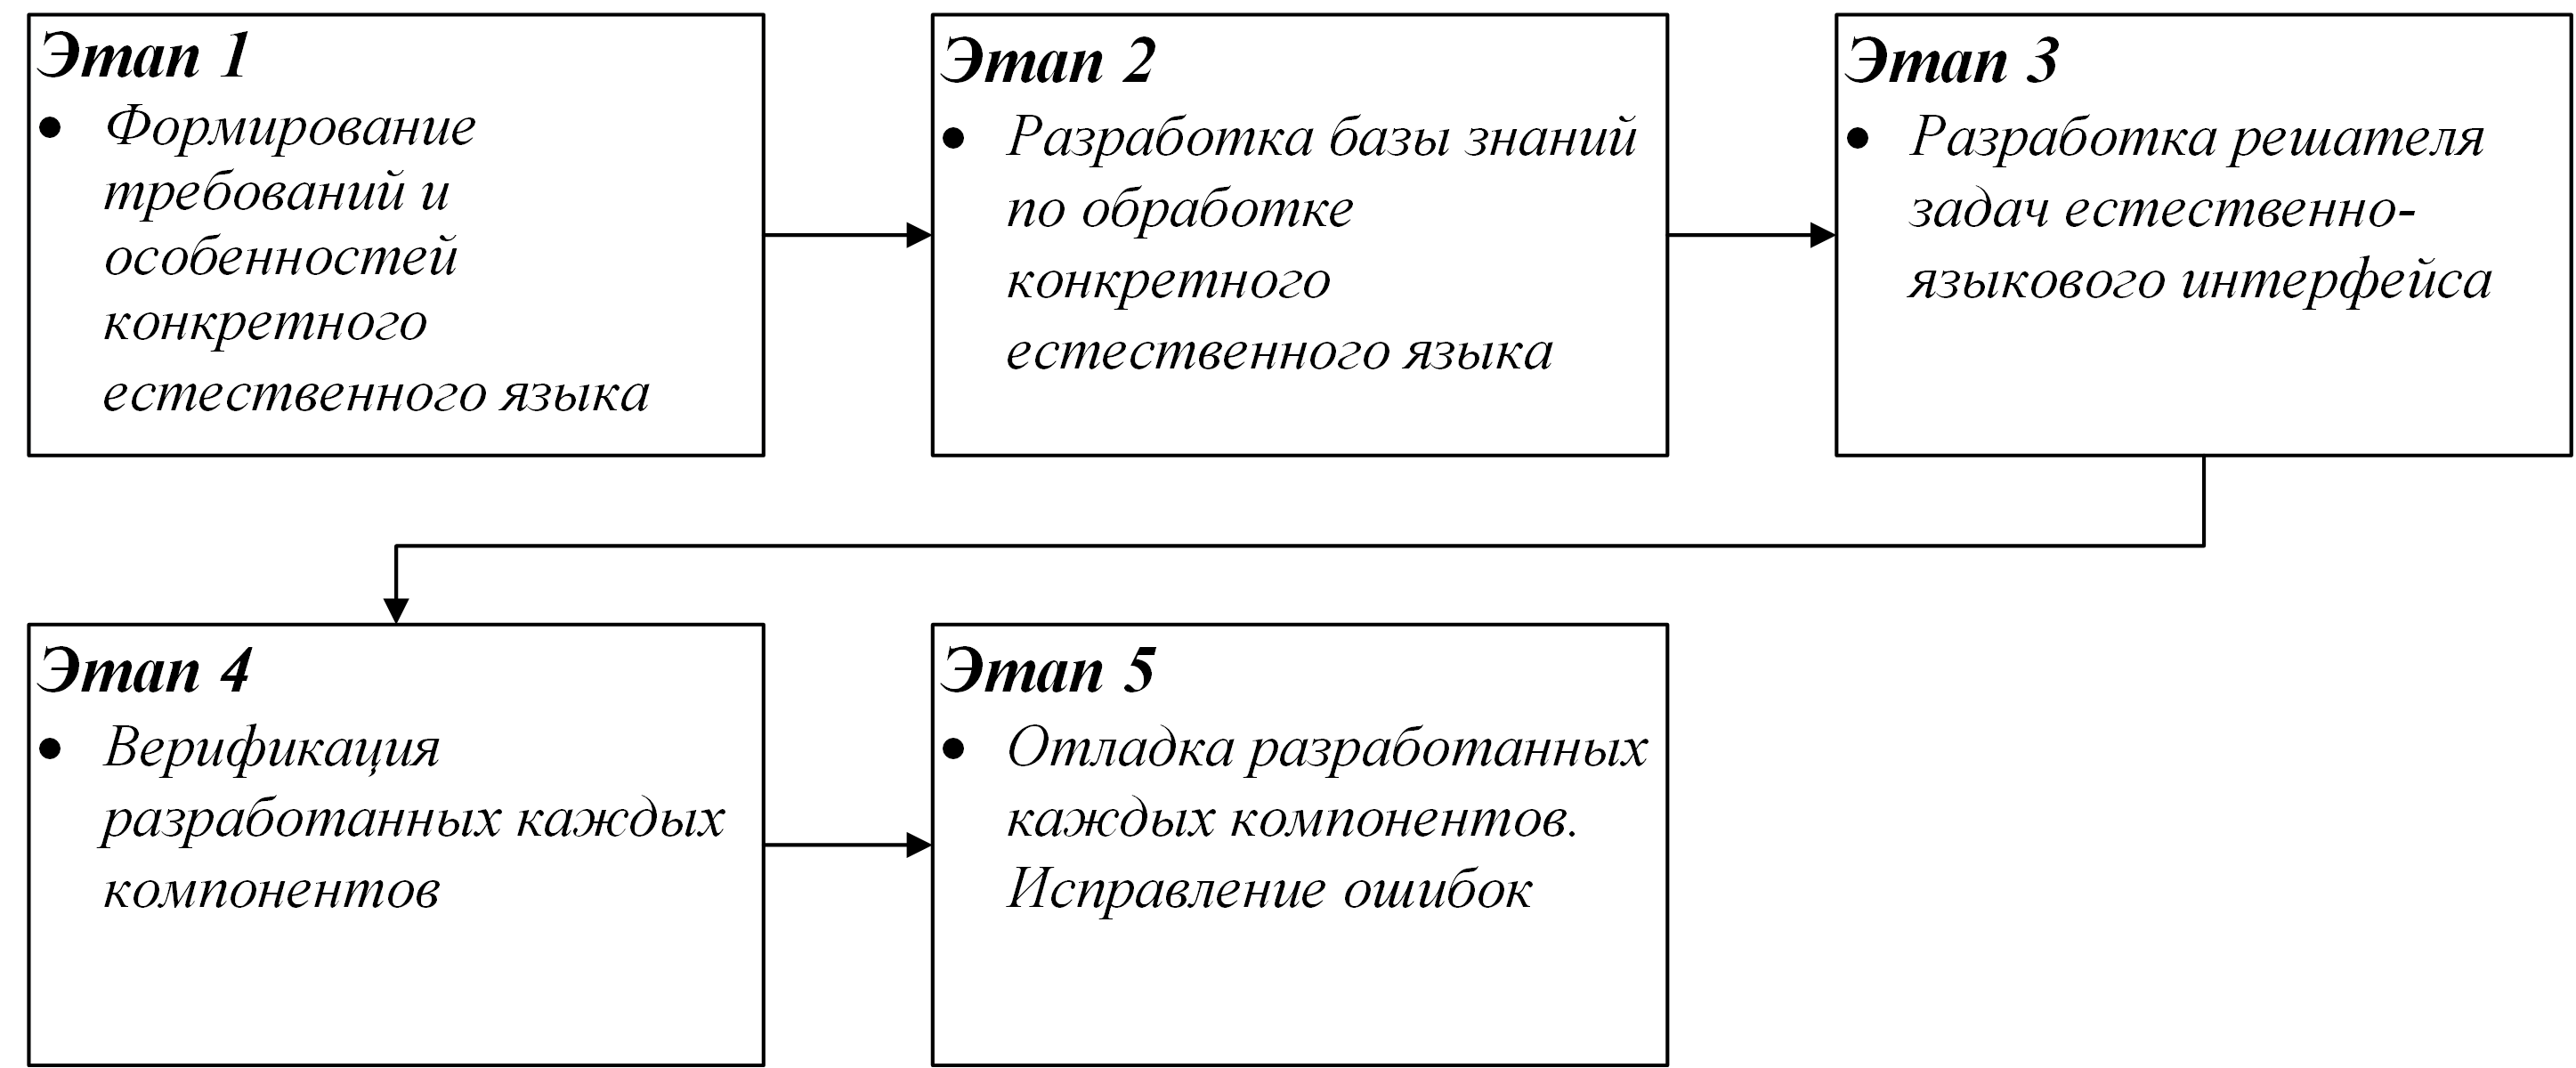
\includegraphics[scale=0.8,width=1.0\textwidth]{images/part4/chapter_chinese/method.png}
	\caption{Этапы процесса разработки естественно-языкового интерфейса}
	\label{fig:method-interface}
\end{figure}

Данная методика может быть применена при разработке конкретного естественно-языкового интерфейса по конкретной предметной области. Далее рассмотрим процесс разработки естественно-языкового интерфейса ostis-систем на этапах:

\textbf{Этап 1. Формирование требований и особенностей конкретного естественного языка.}

На данном этапе необходимо четко рассматривать особенности конкретного естественного языка. Затем можно разработать базу знаний по обработке конкретного естественного языка и соответствующие решатели задач для обработки конкретного естественного языка. После определения конкретного естественного языка существует вероятность того, что в составе библиотеки компонентов уже есть реализованный вариант требуемой базы знаний и соответствующих решателей. В противном случае, тем не менее, у разработчика появляется возможность включить разработанную базу знаний по обработке конкретного естественного языка и соответствующие решатели задач в библиотеку компонентов для последующего использования.

\textbf{Этап 2. Разработка базы знаний по обработке конкретного естественного языка.}

Общие принципы на основе методики согласованного построения и модификации гибридных баз знаний (см. \scncite{Davydenko2017}) используются для разработки базы знаний по обработке конкретного естественного языка.

\textbf{Этап 3. Разработка решателей задач естественно-языковых интерфейсов.}

Общие принципы на основе методики согласованного построения и модификации гибридных решателей задач (см. \scncite{Shunkevich2018}) используются для разработки решателей задач естественно-языкового интерфейса для решения задач приобретения фактографических знаний и генерации текстов конкретного естественного языка.

\textbf{Этап 4. Верификация разработанных каждых компонентов.}

На данном этапе верификация разработанных компонентов (база знаний по обработке конкретного естественного языка и соответствующие решатели задач для решения задач приобретения фактографических знаний и генерации текстов конкретного естественного языка) конкретного естественно-языкового интерфейса может осуществляться вручную

\textbf{Этап 5. Отладка разработанных каждых компонентов. Исправление ошибок.}

Как правило, этапы 4, 5 могут выполняться циклически до тех пор, пока разработанные компоненты не будут соответствовать предъявляемым требованиям.

Библиотека многократно используемых компонентов является важнейшим понятием в рамках технологии OSTIS. С помощью Библиотеки многократно используемых компонентов естественно-языковых интерфейсов могут выбрать компоненты по требованию или набору компонентов в одной из библиотек и включить их в разрабатываемой конкретной естественно-языковой интерфейс других ostis-систем, т.е. разработанные компоненты естественно-языковых интерфейсов могут быть повторно использован при разработке естественно-языковых интерфейсов в других ostis-системах. Аналогично, для разработки конкретных естественно-языковых интерфейсов в других ostis-системах Библиотеки многократно используемых компонентов конкретных естественно-языковых интерфейсов тоже могут использованы повторно для сокращения сроки и трудоемкости разработки конкретных естественно-языковых интерфейсов. Была разработана Библиотеки многократно используемых компонентов естественно-языковых интерфейсов и Библиотеки многократно используемых компонентов китайско-языкового интерфейса в качестве средства для разработки естественно-языковых интерфейсов.
\begin{SCn}
	\scnheader{Библиотека многократно используемых компонентов естественно-языковых интерфейсов}
	\begin{scnrelfromset}{разбиение}
		\scnitem{Библиотека многократно используемых компонентов базы знаний естественно-языковых интерфейсов}
		\begin{scnindent}
			\scnidtf{Библиотека многократно используемых компонентов базы знаний лигвистики}
			\scnidtf{Библиотека многократно используемых компонентов базы знаний по обработке естественного языка}
		\end{scnindent}
		\scnitem{Библиотека многократно используемых компонентов решателей задач естественно-языковых интерфейсов}
		\begin{scnindent}
			\scnidtf{Библиотека многократно используемых компонентов решателей задач для обработки естественного языка}
		\end{scnindent}
	\end{scnrelfromset}
\end{SCn}

\begin{SCn}
	\scnheader{Библиотека многократно используемых компонентов китайско-языкового интерфейса}
	\begin{scnrelfromset}{разбиение}
		\scnitem{Библиотека многократно используемых компонентов базы знаний китайско-языкового интерфейса}
		\begin{scnindent}
			\scnidtf{Библиотека многократно используемых компонентов базы знаний по обработке китайского языка}
		\end{scnindent}
		\scnitem{Библиотека многократно используемых компонентов решателей задач китайско-языкового интерфейса}
		\begin{scnindent}
			\scnidtf{Библиотека многократно используемых компонентов решателей задач для обработки китайского языка}
		\end{scnindent}
	\end{scnrelfromset}
\end{SCn}

На данный момент на основе модели базы знаний лингвистики были разработаны онтологии предметных областей в качестве компонентов, описывающих различные виды лингвистических знаний, которые могут использоваться для реализации конкретных естественно-языковых интерфейсов:
\begin{scnitemize}
	\item Предметная область слов;
	\item Предметная область словосочетаний;
	\item Предметная область предложений;
	\item Предметная область параграфов;
	\item и другие.
\end{scnitemize}

Различные виды лингвистических знаний для обработки китайского языка были специфицированы с использованием разработанных онтологий предметных областей в базе знаний по обработке китайского языка, которые могут быть разработаны в качестве компонентов для разработки китайско-языкового интерфейса в большинстве других ostis-систем.
\begin{scnitemize}
	\item Предметная область единиц сегментации;
	\item Предметная область словосочетаний китайского языка;
	\item Предметная область предложений китайского языка;
	\item Предметная область параграфов китайского языка;
	\item и другие.
\end{scnitemize}

На данный момент на основе модели решателей задач естественно-языковых интерфейсов основное внимание уделено многократно используемым sc-агентам, входящим в состав решателей задач естественно-языковых интерфейсов:
\begin{SCn}
	\scnheader{Библиотека многократно используемых атомарных абстрактных sc-агентов естественно-языковых интерфейсов}
	\begin{scnrelfromset}{разбиение}
		\scnitem{Библиотека sc-агентов формирования структур фактографических знаний}
		\scnitem{Библиотека sc-агентов определения конкретных sc-конструкций}
		\scnitem{Библиотека sc-агентов преобразования sc-конструкций в соответствующие им message triple}
	\end{scnrelfromset}
\end{SCn}

Аналогично, при разработке китайско-языкового интерфейса новой ostis-системы, многократно используемый абстрактный sc-агент нужно быть скопирован в этой новой ostis-системе, после того необходимо сгенерировать sc-узел, обозначающий конкретный sc-агент, работающий в этому китайско-языковом интерфейсе данной системы. На данный момент многократно используемым sc-агентам, входящим в состав решателей задач китайско-языкового интерфейса:
\begin{SCn}
	\scnheader{Библиотека многократно используемых атомарных абстрактных sc-агентов китайско-языкового интерфейса}
	\scnidtf{Библиотека многократно используемых атомарных абстрактных sc-агентов для обработки китайского языка}
	\begin{scnrelfromset}{разбиение}
		\scnitem{Библиотека sc-агентов разбиения текстов на единицы сегментации}
		\scnitem{Библиотека sc-агентов разметки отдельных единиц сегментации}
		\scnitem{Библиотека sc-агентов перевода конкретных sc-конструкций в соответствующие им message triple на китайском языке}
		\scnitem{Библиотека sc-агентов генерации текстов китайского языка из message triple}
	\end{scnrelfromset}
\end{SCn}

\subsection {Реализация китайско-языкового интерфейса}
На основе sc-модели естественно-языковых интерфейсов ostis-систем могут быть реализованы конкретные естественно-языковые интерфейсы интеллектуальных справочных систем по различным предметным областям. Однако из-за трудоемкости и сложности разработки интеллектуальных справочных систем по конкретным предметным областям, а также автор как носитель китайского языка, прототип китайско-языкового интерфейса был реализован в интеллектуальной справочной системе по дискретной математике.

\subsubsection{Извлечение фактографических знаний из текстов китайского языка}
Преобразование текстов естественного языка в фрагменты базы знаний рассматривается как задачи извлечения фактографических знаний. В данном случае преобразование текстов китайского языка в фрагменты базы знаний интеллектуальной справочной системы по дискретной математике заключается в извлечении именованных сущностей и отношений между ними из текстов китайского языка по дискретной математике, а наконец извлеченные результаты сохраняются в виде SC-кода в базе знаний интеллектуальной справочной системы по дискретной математике.

Несколько требований былы определены для задач преобразования текстов китайского языка в фрагменты базы знаний:
\begin{textitemize}
	\item Вход представляет собой стандартное повествовательное предложение китайского языка, а не речевое;
	\item Входное повествовательное предложение китайского языка имеет завершенный смысл и фактографическое знание;
	\item Не нужен заранее заданный словарь, включающий заранее определенные типы именованных сущностей и отношений между ними;
	\item Выход представляет собой sc-структура, формально представленная в базе знаний.
\end{textitemize}

В данном подразделе показан пример процесса анализа предложения китайского языка, которое представлено на таком узле на рисунке \textit{\nameref{fig:chinese-sentence-sc}}. Содержимое такого узла демонстрирует предложение китайского языка, которое относится к области дискретной математики и описывает: \begin{CJK}{UTF8}{gbsn}«从结构形式化的角度 (с точки зрения формализации структуры) ,结构(структуру) 可以 (можно) 划分 (разделить) 为 (на) 形式化的结构 (формальную структуру) 和 (и) 非形式化的结构 (неформальную структуру) 。». \end{CJK}
\begin{figure}[H]
	\centering
	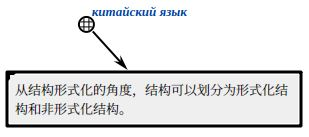
\includegraphics[scale=0.8]{images/part4/chapter_chinese/chinese_sentence.png}
	\caption{Представление предложения китайского языка в ostis-системе}
	\label{fig:chinese-sentence-sc}
\end{figure}

\textbf{\textit{Шаг 1:}} Декомпозиция предложения китайского языка на отдельные единицы сегментаций, а также помечаются данные единицы сегментаций стандартными категориями частей речи в китайском языке (рисунок \textit{\nameref{fig:segment-chinese}}).
\begin{figure}[H]
	\centering
	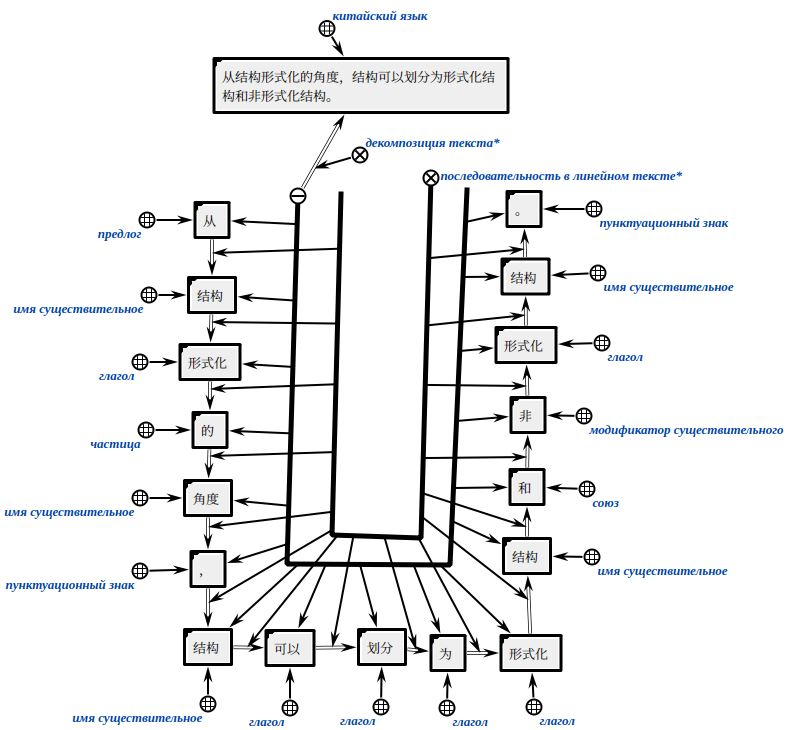
\includegraphics[scale=0.6]{images/part4/chapter_chinese/segment_chinese_sentence.png}
	\caption{Результат разделения и разметки отдельных единиц сегментации}
	\label{fig:segment-chinese}
\end{figure}

Согласно особенности текстов китайского языка, текст китайского языка состоит из потока иероглифов без естественных пробелов на основе письменной формы. При этом в китайском языке отсутствуют четкие показатели категорий числа, падежа и рода, такие как в русском языке и других европейских языках, функция слова в китайском языке становится понятной не на основании морфологических изменений слова, а благодаря его связи с другими словами. В связи с этим в процессе анализа текстов китайского языка сначала необходимо выполнить лексический анализ, разбивающий поток иероглифов в тексте китайского языка на отдельные значимые единицы сегментации китайского языка. 

\textbf{\textit{Шаг 2:}} Синтаксический анализ выполняет построение синтаксической структуры предложения китайского языка (рисунок \textit{\nameref{fig:syntac-structure}}).

При обработке китайского языка синтаксический анализ являются анализом взаимосвязей (или отношений зависимости) между входными предложениями китайского языка и раздельными единицами сегментаций и между раздельными единицами сегментации в предложениях китайского языка для раскрытия их синтаксических структур. На основе построенной синтаксической структуры приложений китайского языка фактографические знания можно быть извлечены с использованием правил извлечения. Таким образом, синтаксический анализ китайского языка позволяет создать основу для извлечения фактографических знаний из предложений китайского языка.
\begin{figure}[H]
	\centering
	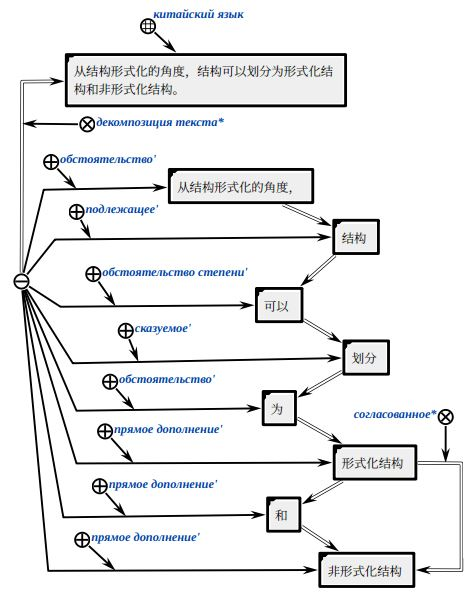
\includegraphics[scale=0.6]{images/part4/chapter_chinese/syntac_structure.png}
	\caption{Результат синтаксического анализа предложения китайского языка}
	\label{fig:syntac-structure}
\end{figure}

При обработке китайского языка отношения между единицами сегментации и входным предложением китайского языка, или отношения между единицами сегментации в предложения китайского языка, обычно рассматриваются как определенные типы лингвистических знаний, включенных в базе знаний по обработке китайского языка.

\textbf{\textit{Шаг 3:}} На основе результата синтаксического анализа входного предложения китайского языка фактографические знания (именованные сущности и отношения между ними) извлекаются из предложения с использованием правил извлечения, т.е. построение фрагмента базы знаний в базе знаний интеллектуальной справочной системы.


\begin{figure}[H]
	\centering
	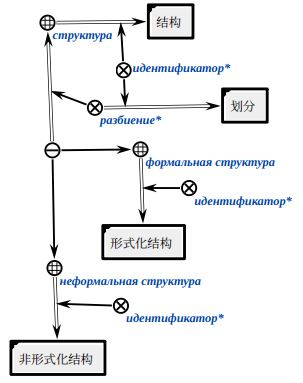
\includegraphics[scale=0.7]{images/part4/chapter_chinese/generated_sc_structure.png}
	\caption{Результирующий построенный фрагмент в базе знаний}
	\label{fig:generated-structure}
\end{figure}

С точки зрения извлечения фактографических знаний из открытой области, основными задачами является извлечение именованных сущностей и отношений между ними из предложений китайского языка, не требуя предопределенных типов именованных сущностей и отношений. Фактически, в рамках \scnkeyword{Технологии OSTIS} отношение рассматривается как специальная сущность, которая определяет определенное отношение между парами независимых именованных сущностей, которое обычно представлена соответственно как sc-узел, обозначающий ролевое отношение в форме SCg-кода.

В целом, пары независимых именных сущностей должны появляться в анализируемой синтаксической структуре в виде именных фраз, относящихся к номинативным единицам. В дальнейшем связи между этими именными фразами и входным предложением китайского языка, а также путь, связывающий две именные фразы через другие единицы сегментаций, будут отражать соответствующие отношения между парами именных сущностей. Более точно, именные фразы, появляющиеся в анализируемой синтаксической структуре входного предложения китайского языка, представляются как идентификаторы sc-узлов, обозначающих название некоторых именованных сущностей, хранящихся в базе знаний интеллектуальной справочной системы по дискретной математике.

На рисунке \textit{\nameref{fig:generated-structure}} показан построенный фрагмент базы знаний из входного предложения китайского языка в базе знаний интеллектуальной справочной системы по дискретной математике без обнаружения противоречий. В данном случае фрагмент базы знаний может быть построен напрямую без связывания именованных сущностей, упомянутых во входном исходном предложении китайского языка, с соответствующими существующими определенными именованными сущностями в базе знаний интеллектуальной справочной системы по дискретной математике. В некоторых случаях для именованной сущности в базе знаний существуют различные названия в текстах естественного языка для описания этой именованной сущности. В этом случае необходимо выполнить устранение противоречий, чтобы связать разные именованные сущности (именно идентификаторы именованных сущностей) в текстах естественного языка с одинаковыми именованными сущностями в базе знаний ostis-системы. 
\subsubsection{Генерация текстов из фрагментов базы знаний}
Для реализации генерации текстов китайского языка из фрагментов базы знаний ostis-системы условно делится на два этапа: символьные генераторы, преобразующие фрагменты (sc-структуры) базы знаний в соответствующие им ``message triple''; генераторы на основе шаблонов или статистические генераторы (при наличии высококачественных выровненных наборов данных), переводящие ``message triple'' в результирующие тексты китайского языка. Пример генерации текстов китайского языка демонстрирует процесс генерации повествовательного предложения китайского языка на основе правил и шаблонов.

Из-за сложности и разнообразия задач генерации текстов, при генерации текстов китайского языка из фрагментов базы знаний ostis-системы соблюдаются следующие ограничения:
\begin{textitemize}
	\item входной фрагмент базы знаний обладает законченной sc-структурой и конкретным смыслом;
	\item выходным результатом является повествовательное предложение китайского языка;
	\item входной фрагмент базы знаний содержит sc-элементы (представляющие сущности, отношения, класс сущностей или другие) с идентификаторами на китайском языке, которые будут использоваться в результирующих предложениях китайского языка.
\end{textitemize}

\textbf{\textit{Шаг 1:}} Локализация заданного фрагмента (sc-структура) из базы знаний интеллектуальной справочной системы по дискретной математике, представленного в виде SC-кода и содержащего sc-элементы с идентификаторами на китайском языке. Для визуального представления данного фрагмента базы знаний, фрагмент формально представлен на SCg-коде (рисунок \textit{\nameref{fig:knowledge-base-fragment}}).
\begin{figure}[H]
	\centering
	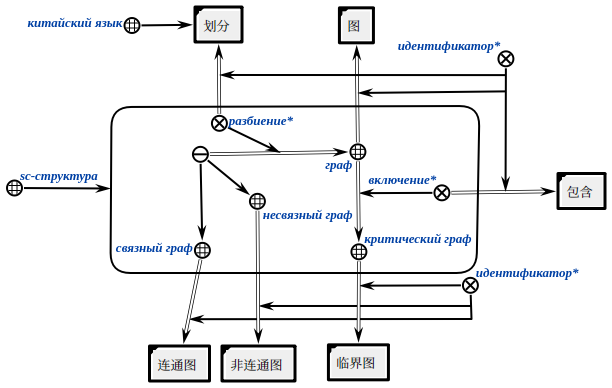
\includegraphics[scale=0.7]{images/part4/chapter_chinese/fragment_knowledge_base.png}
	\caption{Фрагмент (sc-структура) базы знаний ИСС по дискретной математике}
	\label{fig:knowledge-base-fragment}
\end{figure}

\textbf{\textit{Шаг 2:}} Данный фрагмент разделяется на стандартные базовые sc-конструкции, из которых выбираются проектные sc-конструкции для генерации результирующих текстов китайского языка, которые можно переводиться в ``message triple''. У каждого sc-элемента sc-конструкций есть конкретная единица сегментации китайского языка, соответствующая идентификатору каждого sc-элемента. Проектная sc-конструкция (принадлежащая к стандартной базовой sc-конструкции) показана на SCg-коде (рисунок \textit{\nameref{fig:candidate-sc-construction}}).
\begin{figure}[H]
	\centering
	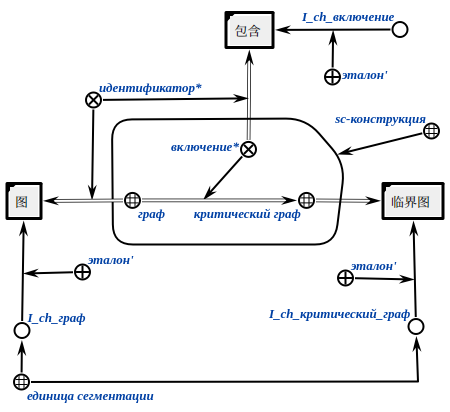
\includegraphics[scale=0.8]{images/part4/chapter_chinese/candidate_sc_structure.png}
	\caption{Выбранная проектная sc-конструкция}
	\label{fig:candidate-sc-construction}
\end{figure}

\textbf{\textit{Шаг 3:}} Проектная sc-конструкция переносится в ``message triple''. Преобразованный ``message triple'' состоит из файлов (sc-узел с содержимым), содержащих единицы сегментаций, написанные обученными носителями китайского языка и проверенной другими. Содержимое некоторых файлов (например \begin{CJK}{UTF8}{gbsn} «临界图 (критический граф)» \end{CJK}) соответствует идентификатору sc-элементов sc-конструкций, а содержимое некоторых файлов добавляется при построении ``message triple''. (рисунок \textit{\nameref{fig:message-triple}}).
\begin{figure}[H]
	\centering
	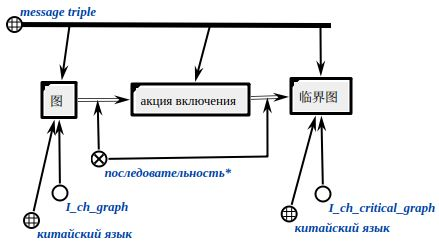
\includegraphics[scale=0.7]{images/part4/chapter_chinese/message_triple.png}
	\caption{Перевод проектной sc-конструкции в ``message triple''}
	\label{fig:message-triple}
\end{figure}

\textbf{\textit{Шаг 4:}} файлы объединяются для генерации результирующего повествовательного предложения китайского языка в соответствии с допустимыми упорядоченностями на шаблоне для ``message triple'' с отношением «включение» (рисунок \textit{\nameref{fig:sentence-generated}}). При генерации результирующих текстов для некоторых естественных языков Формы слов изменяются в соответствии с правилами (например, заглавная буква первого слова в предложении, согласование сказуемого с подлежащим), а затем добавляются в результирующие тексты. \textit{ссылающееся выражение*} -- квазибинарное отношение, связывающее слово с её комбинаторными вариантами.
\begin{figure}[H]
	\centering
	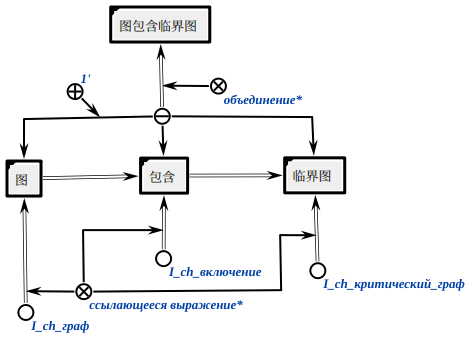
\includegraphics[scale=0.7]{images/part4/chapter_chinese/chinese_sentence_generated.png}
	\caption{Генерация предложения китайского языка, соответствующего sc-структуре}
	\label{fig:sentence-generated}
\end{figure}

В отличие от европейских языков, склоняемая форма лексических единиц (например, единственного или множественного числа и других форм склонения) в файлах указывается в результирующих текстах в соответствии с синтаксическими правилами конкретного естественного языка. Однако в связи с особенностями китайского языка, обработка данного шага относительно проще. В данном примере при генерации результирующего предложения китайского языка, ссылочное выражение каждой единицы сегментации означает конечную форму единицы сегментации в результирующем предложении китайского языка. Исходя из шаблона, в качестве подлежащего выступает ссылочное выражение к единице сегментации \begin{CJK}{UTF8}{gbsn} «图 (граф)» \end{CJK}. Единица сегментации \begin{CJK}{UTF8}{gbsn} «临界图 (критический граф)» \end{CJK} выступает в качестве объекта. Сгенерированное предложение китайского языка описывает \begin{CJK}{UTF8}{gbsn}«图 (граф) 包含 (включение) 临界图 (критический граф)». \end{CJK}

Некоторые отношения уже предопределены в \scnkeyword{IMS} (см. \scncite{IMS}) системе для разработки ostis-системы, так \textit{включение*}, \textit{эквиваленция*} и так далее. Для данных конечных отношений, предопределенных в \scnkeyword{IMS} системе, будем называть доменно-независимые отношения. Для бесконечных доменно-зависимых отношений в различных предметных областей модель нейронной сети интегрирована в решатель задач к генерации текстов китайского языка. На рисунке \textit{\nameref{fig:pre-training-model}} показан процесс использовании формы предварительной подготовки и тонкой настройки для решения задач генерации текстов китайского языка из фрагментов базы знаний. 
\begin{figure}[H]
	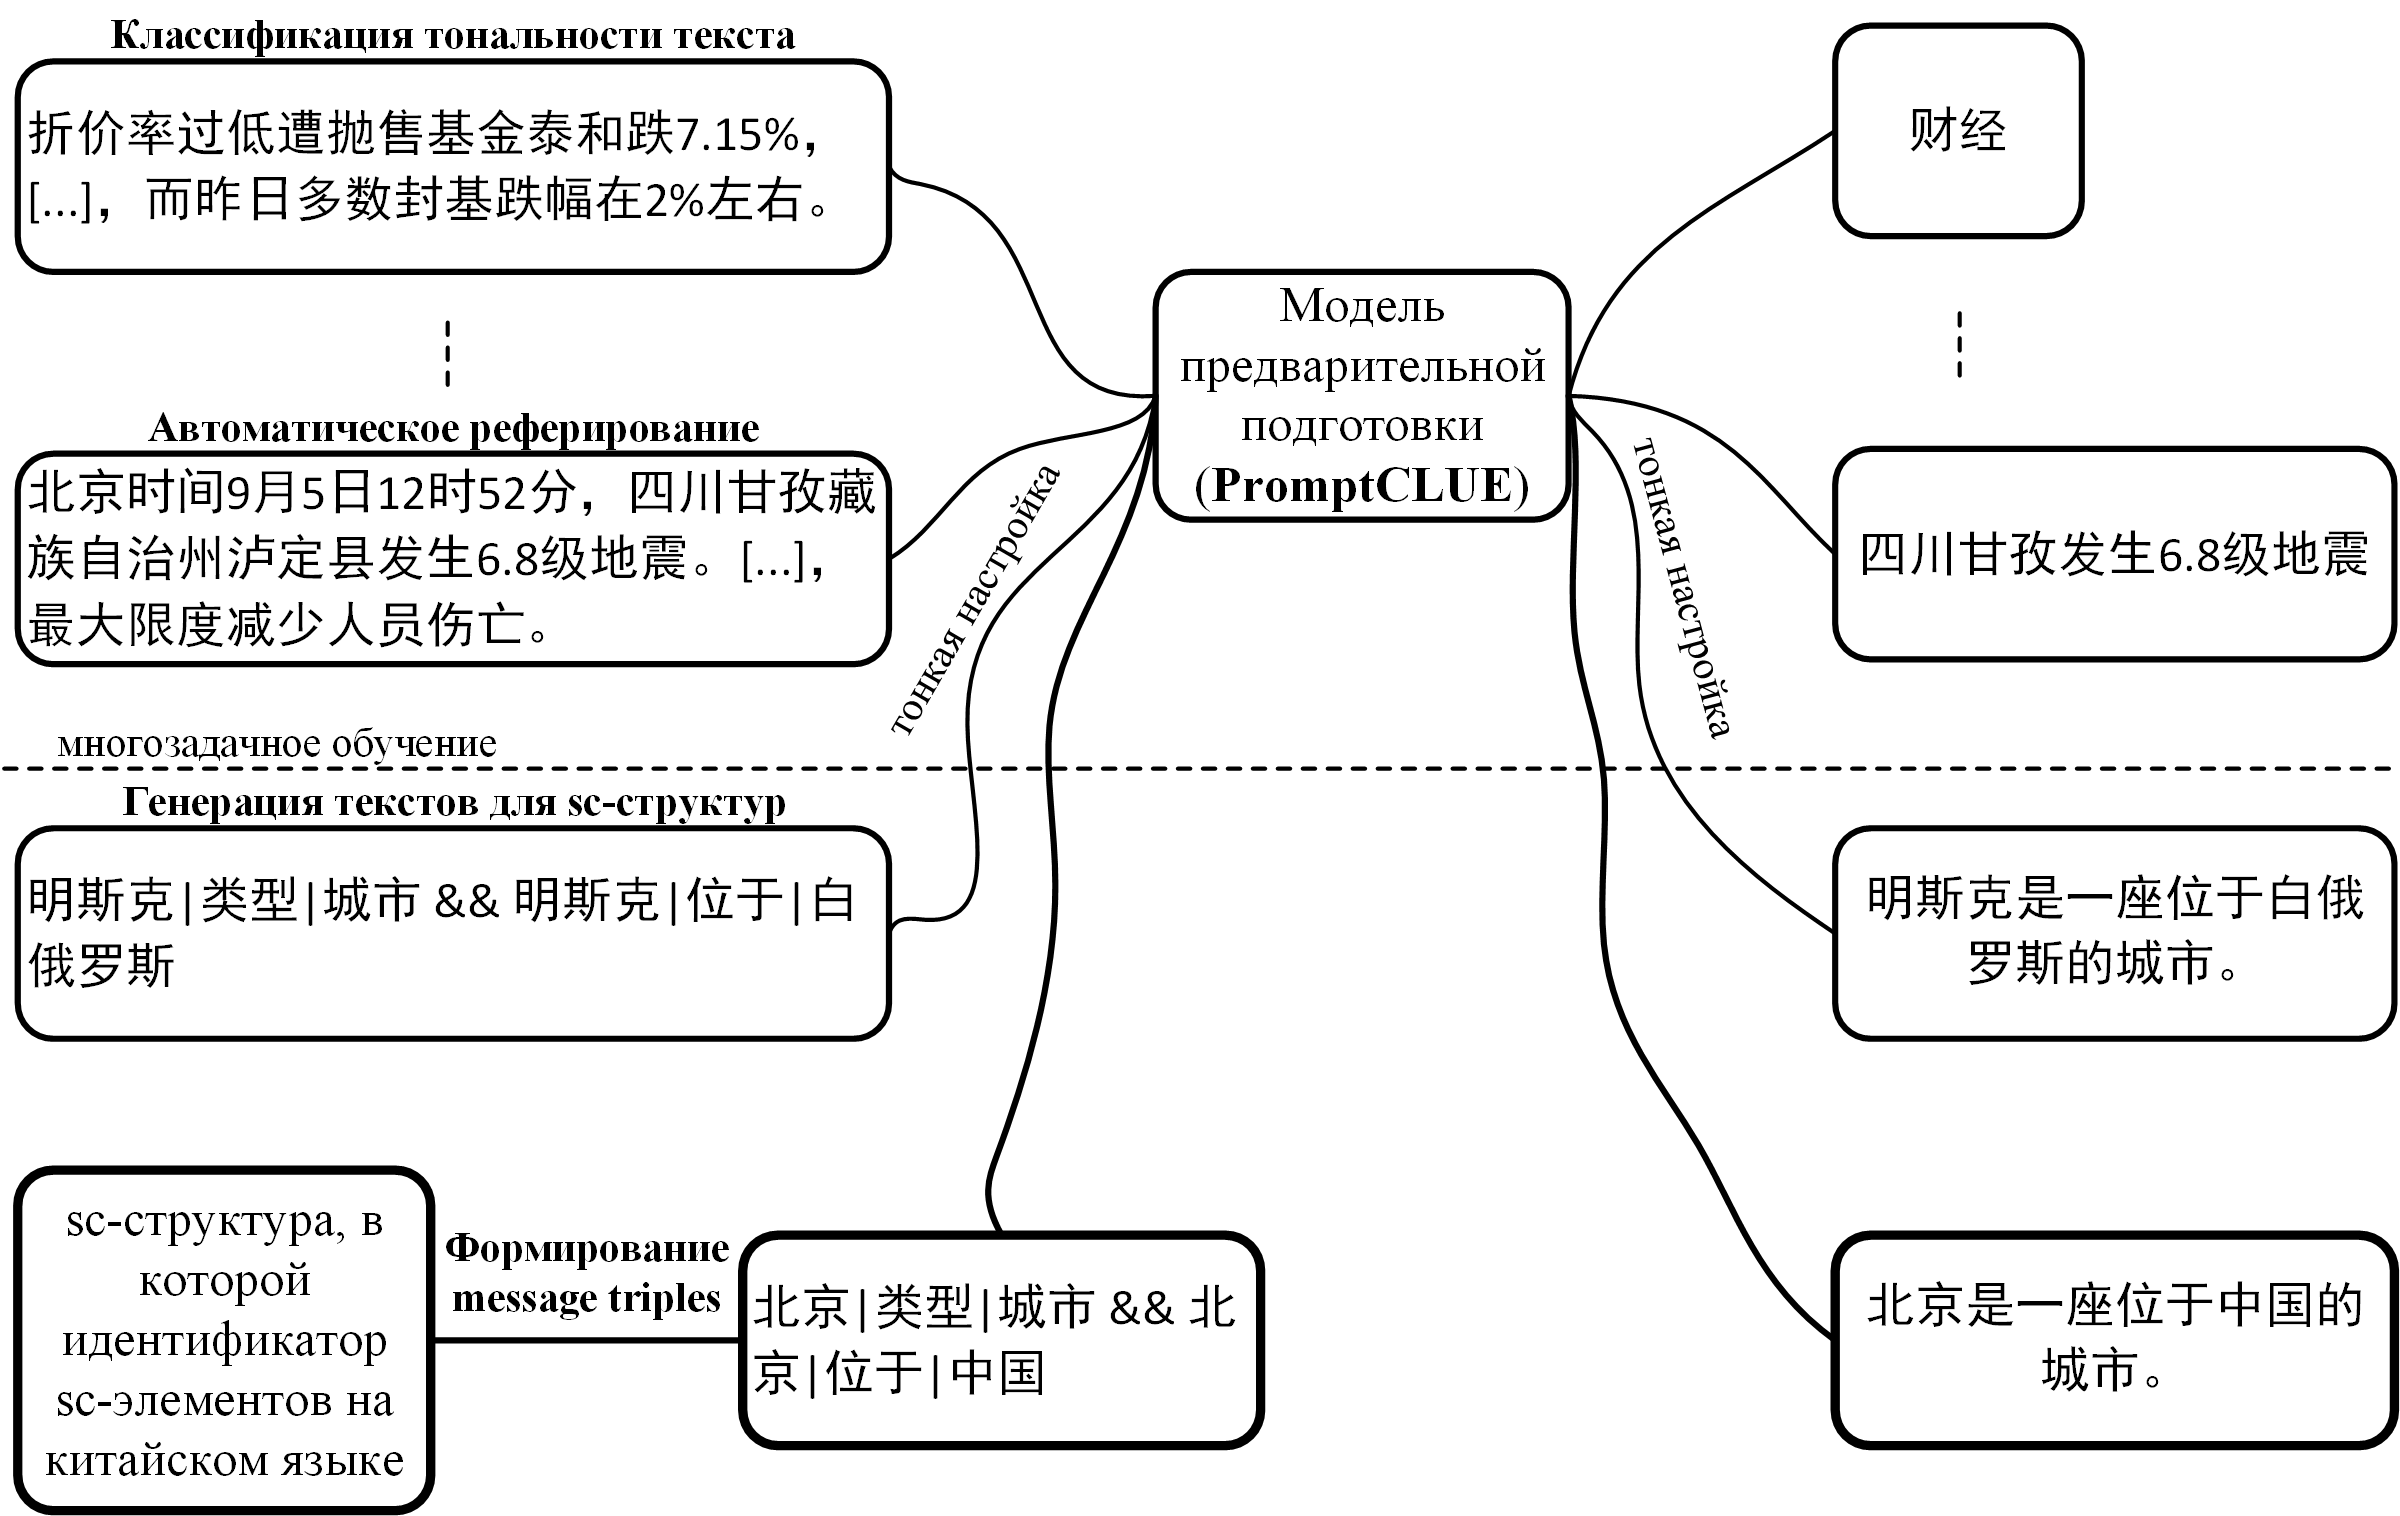
\includegraphics[scale=0.8,width=1.0\textwidth]{images/part4/chapter_chinese/promptCLUE4SC.png}
	\caption{Диаграмма для генерации текстов на основе модели предварительной подготовки PromptCLUE}
	\label{fig:pre-training-model}
\end{figure}

Как видно из рисунка \textit{\nameref{fig:pre-training-model}}, была использована модель предварительной подготовки PromptCLUE, которая использует еncoder-decoder архитектуру на основе модели Transformer и предварительно обучается на нескольких наборов задач про обработке китайского языка (классификация тональности текста, автоматическое реферирование и другие) с использованием огромного китайского корпуса (сотни ГБ китайского корпуса).  На основе модели PromptCLUE, проведена тонкая настройка с использованием построенных корпусов для генерации текстов китайского языка из фрагментов базы знаний (sc-структур) в виде пары ``message triple''/предложение китайского языка. После обучения тонкой настройки на модели PromptCLUE, обученная модель может быть использована для генерации текстов китайского языка после предварительной обработки sc-структур в ``message triple''. 

\section*{Заключение}
В главе предложена на основе \scnkeyword{Технологии OSTIS} единая семантическая модель естественно-языковых интерфейсов интеллектуальных систем для разработки естественно-языковых интерфейсов, которые имеют возможность преобразовывать тексты естественного языка в фрагменты базы знаний и генерировать тексты естественного языка из фрагментов базы знаний интеллектуальных систем. Разработка семантической модели естественно-языковых интерфейсов в основном включает разработку SC-модели базы знаний лингвистики, которая представлена в виде описанных предметных областей и соответствующих им онтологий по лингвистическим знаниям для обработки естественного языка, а также SC-модели решателя задач естественно-языковых интерфейсов, разработанной как иерархическая система sc-агентов и позволяющей интегрировать различные модели решения задач (например логические модели на основе правил, модели нейронных сетей и другие) для обработки естественного языка.

С помощью предложенной семантической модели естественно-языковых интерфейсов реализован прототип китайско–языкового интерфейса ИСС по дискретной математике, способный решать задачи преобразования текстов китайского языка в фрагменты базы знаний и генерации текстов китайского языка из фрагментов базы знаний. Для реализации китайско–языкового интерфейса разработана база знаний по обработке китайского языка и соответствующие решатели задач анализа текстов и генерации текстов китайского языка.
%\input{author/references}
\chapter{Аудиоинтерфейс ostis-систем}
\chapauthortoc{Азаров И.С.\\Вашкевич М.И.\\Захарьев В.А.\\Лихачев Д.С.\\Петровский Н.А.}
\label{chapter_audio_interfaces}

\vspace{-7\baselineskip}

\begin{SCn}
\begin{scnrelfromlist}{авторы}
    \scnitem{Азаров И.С.}
    \scnitem{Вашкевич М.И.}
    \scnitem{Захарьев В.А.}
    \scnitem{Лихачев Д.С.}
    \scnitem{Петровский Н.А.}
\end{scnrelfromlist}

\bigskip

\scntext{аннотация}{Данная глава посвящена рассмотрению вопросов создания аудио и речевых интерфейсов для интеллектуальных компьютерных систем нового поколения. Предлагается использование подхода на основе онтологического проектирования и формализации системы понятий из предметной области аудиоинтерфейсов, посредством технологии OSTIS.  Изложены основные идеи лежащие в основе данного подхода, а также их отличительные особенности от общепринятых. Показано, что в перспективе, использование данного подхода может обеспечить свойства унификации, семантической совместимости и интероперабельности, при разработке аудио и речевых интерфейсов, что в итоге позволит существенным образом сократить издержки при создании интеллектуальных компьютерных систем нового поколения для решении комплексных задач.}

\bigskip

\begin{scnrelfromlist}{ключевое понятие}
    \scnitem{аудио интерфейс интеллектуальных компьютерных систем}
    \scnitem{речевой интерфейс интеллектуальных компьютерных систем}
    \scnitem{цифровая обработка сигналов}
    \scnitem{обработка речевых сигналов}
\end{scnrelfromlist}

\bigskip

\begin{scnrelfromlist}{библиографическая ссылка}
        \scnitem{\scncite{Pearl2016}}
        \scnitem{\scncite{Chen2021audio}}
        \scnitem{\scncite{Lu2002content}}
        \scnitem{\scncite{Fernandes2022}}
\end{scnrelfromlist}

\end{SCn}


\section{Анализ существующих подходов к разработке аудиоинтерфейсов интеллектуальных компьютерных систем}

Разговорная речь является одной из наиболее естественных и эффективных форм передачи информации между людьми. Этот факт объясняет значительный интерес исследователей к вопросам развития и применения речевых интерфейсов для обеспечения человеко-машинного взаимодействия в составе современных коммуникационных, мультимедийных и интеллектуальных систем (см. \scncite{Pearl2016}, \scncite{Chen2021audio}).

Более всеобъемлеющей формой обеспечения взаимодейтсвия с пользователем и окружающей средой по средствам анализа и синтеза акустических сигналов является аудиоинтерфейс. Данную разновидность интерфейса, выступающей родительской по отношению к речевым, можно кратко определеить как аппаратно-программный комплекс осуществляющий анализ и синтез сигналов во всем доступном спектре параметров носителей акустической информации. Например, для решения задач анализа обстановки и событий происходящех в акустическом окружении системы, синатеза неречевых сигналов (звуков техногенного и природного характера, сигналов оповещения, музыки, и т.д.) (см. \scncite{Lu2002content}).

Об акутальности направления разработки аудио и речевых интерефейсов свидетельствуют следующие основные тенденции развития данного направления:
\begin{textitemize}    
    \item экономические показатели и прогнозы развития рынка речевых технологий, текщие среднегодовые темпы роста которого, по оценкам экспертов, составляют порядка 22\%, а совокупный объём будет равен 59,6 млрд. долл. США к 2030 (см. \scncite{Fernandes2022});
    \item появление широкого спектра продуктов на основе речевого интерфейса, получивших массовое распространение. В первую очередь это персональные голосовые асситенты, таких как  «Alexa» (Amazon), «Siri» (Apple), «Сortana» (MicroSoft), «Алиса» (Yandex) (см. \scncite{Bellegarda2014}, \scncite{Lemley2017}, \scncite{Hoy2018});
    \item интерес со стороны научного сообщества, выражающийся в росте публикаций в этом напрвлении исследований на 15\% за последние 5 лет (см. \scncite{Semscholar2022stat}).
\end{textitemize}

Необходимо отметить, что основная масса научных публикаций в данном направлении посвящена развитию базовых технологий, являющихся составляющими речевого интерфейса, таким как синтез речи по тексту, а также распознавание речи в текст (см. \scncite{Popov2020interspeech}, \scncite{Povey2011ASRU}, \scncite{Deepa2021}). Последние достижения в этих направлениях, связанны с бурным развитием нейросетевых моделей и вычислительных средств. Они позволили довести качественные характеристики использования речевых технологий до комерческого уровня (см. \scncite{Vosk2021}, \scncite{Radford2022robust}).

Большиство существующих систем, как правило, рассчитаны на решение опрёдленного круга задач и сложно совместимы друг другом. Данный факт в особенности остро проявляется при проектировании сложных систем, наподобие интеллектуальных персональных диалоговых ассистентов, требующих использования многообразия различных видов обрабатываемой информации и различных моделей решения задач. Такие системы кроме стандартных модулей распознавания (ASR, automatic speech recognition) и синтеза (TTS, text to speech), на уровне аудиоинтерфейса также должны содержать модели, определяющие наличие/отсутсвие речи в аудиосигнале в сложной акустической обстановке, классификации звуков окружающей среды, распознавание диктора и пр. Помимо этого элементы речевого интерфейса должны быть совместимы с более высокоуровневыми модулями обработки естественно-языковой информации, такими как модули понимания (SLU, spoken language understanding) и генерации речи (SLG, spoken language generation), управления диалогом (DM, dialog manager) (см. \scncite{Delic2019speech}). 

Всё это требует разработки подходов основанных не только на методах машинного обучения и обработке сигналов, но и обработки естесвенного языка, символических методах искуственного интеллекта, онтологическмо проектировании и формализации предметной области аудиоинтерфейса. Это позволит создать системы, которые обладают полным спектром знаний в формализованном виде о типах задач которые они должны решать и методах доступных для их решения.

Необходимым условием для создания таких систем нового покаления, обладающих улучшенными характеристиками по критериям интероперабельности и гибкости является также тот факт, что данные системы должны быть построены на основе базовой технологии, позволяющей обеспечить такое единство формы представления информации на всех её уровнях.
 
Совокупность данных факторов приводит к необходимости создания интеллектуальных компьютерных систем нового поколения, которые будут включать в себя модули аудио и речевого интерфейса, построеные на основе принципов интероперабельности и семантической совместимости для решения комплексных задач.


\section{Применение принципов онтологического проектирования при разработке аудиоинтерфейсов}

Для достижения поставленной цели предлагается прибегнуть к подходу на основе принципов лежащих в основе ``Стандарта открытой технологии онтологического проектирования, производства и эксплуатации семантически совместимых гибридных интеллектуальных компьютерных систем'' или кратко ``Стандарта технологии OSTIS''.

Суть подхода заключается в рассмотрении процесса проектирования аудиоинтерфейса как интерфейсной подсистемы в рамках общего процесса разработки интеллектуальной компьютерной системы (ИКС) и построении её формальной логико-семантической модели.

Для создания подобной модели интеллектуальной компьютерных систем нового поколения необходимо:
\begin{textitemize}    
    \item произвести декомпозицию информационной компьютерной системы на компоненты. Качество декомпозии при этом определяется простотой последующего синтеза общей формальной модели из формальных моделей выделенных компонентов.
    \item провести конвергенцию выделенных компонентов в целях построения совместимых (легко интегрируемых) формальных моделей этих компонентов;
    \item провести интеграцию построенных формальных моделей выделенных компонентов и получить общую формальную модель.
\end{textitemize}

Общими методологическими принципами, являющимися основой перехода к ИКС нового поколения при этом являются:
\begin{textitemize}    
    \item конвергенция и унификация ИКС и их компонентов;
    \item структурно-системное упрощение ИКС (принцип "Бритвы Оккама"{});
    \item ориентация на универсальные ИКС;
    \item синтез ИКС из совместимых компонентов;
    \item ориентация на создание синергетических ИКС.
\end{textitemize}

Из общих методологических принципов вытекают следующие важные особенности предлагаемого подхода, которым необходимо следовать для достижения поставленной цели.
\begin{textitemize}    
    \item смысловое представление знаний;
    \item агентно-ориентированная базовая модель обработки баз знаний, имеющих смысловое представление (инсерционное программирование в смысловом пространстве);
    \item семантическая структуризация баз знаний в виде иерархической системы предметных областей и соответствующих им онтологий, специфицирующих эти предметные области;
    \item интерфейс ИКС нового поколения, при этом, трактуется как специализированная интеллектуальная информационная система, ориентированная на решение интерфейсных задач соответствующей индивидуальной ИКС и глубоко интегрированная (встроенная) в эту ИКС.
\end{textitemize}

 В качестве технологической основы для реализации предлагаемого подхода будет использоваться Технология OSTIS (см. \scncite{Standart2021}). Системы, построенные на основе Технологии OSTIS, названы OSTIS-системами, соответственно подсистема аудиоинтерфейса, будет строиться как многократно используемый компонент, который в будущем будет при необходимости встраиваться в различные OSTIS-системы.

В качестве формальной основы для кодирования различной информации в базе знаний используется SC-код , тексты которого (sc-тексты) записываются в виде семантических сетей с базовой теоретико-множественной интерпретацией. Элементы таких сетей получили название sc-элементов (sc-узлов, sc-дуг).

Ориентация данной работы на Технологию OSTIS обусловлена ее следующими основными преимуществами:
\begin{textitemize}
\item в рамках указанной технологии предложены унифицированные средства представления различных видов знаний, в том числе - метазнаний, что позволить описать всю необходимую для анализа информацию в одной базе знаний в едином ключе (см. \scncite{Davydenko2017});
\item используемый в рамках технологии формализм позволяет специфицировать в базе знаний не только понятия, но и любые внешние с точки зрения базы знаний файлы (например, фрагменты речевого сигнала), в том числе - синтаксическую структуру таких файлов;
\item предложенный в рамках технологии подход к представлению различных видов знаний (см. \scncite{Davydenko2017}) и моделей их обработки (см. \scncite{Shunkevich2018}) обеспечивает модифицируемость OSTIS-систем, т.е. позволяет легко расширять функциональные возможности системы, вводя новые виды знаний (новые системы понятий) и новые модели обработки знаний;
\end{textitemize}

В данном разделе монографии, в отличие от предыдущих работ авторов, посвященных вопросам семантического анализа голосовых сообщений на основе формализованного контекста и создания диалоговых ассистентов на основе модели ментального лексикона или мультимодальной системы на основе нейросемволического подхода, технология OSTIS используется для непосредственного построения онтологии подсистемы аудио интерфейса (см. \scncite{Zahariev2018}, \scncite{Zahariev2019}, \scncite{Zahariev2020}, \scncite{Zahariev2021}).

Поскольку аудиоинтерфейс ИКС нового поколения должен иметь архитектуру, соответсвующую общим правилам построения OSTIS-систем, можно выделить и формализовать следюущие осеовные его части: 
\begin{SCn}
	\scnheader{Аудиоинтерфейс интеллектуальных компьютерных систем нового поколения}
	\scntext{сокращение}{аудиоинтерфейс ИКС}
	\begin{scnrelfromset}{обобщенная декомпозиция}
		\scnitem{база знаний подсистемы аудиоинтерфейса ИКС нового поколения}
		\scnitem{решатель задач подсистемы аудиоинтерфейса ИКС нового поколения}
		\scnitem{интерфейс для взаимодействия с остальными интерфейсными подсистемами OSTIS-системы}
	\end{scnrelfromset}
\end{SCn}

Таким образом неободимо отметить что процесс разработки аудиоинтерфейса для ИКС нового поколения, подразумевает прежде всего создание семантически структуризованных баз знаний в виде иерархической системы предметных областей и соответствующих им онтологий, специфицирующих эти предметные области. Следовательно, первым шагом для достижения поставленной цели должен являться этап выделения и формализации сущностей аудио и речевого интерфейса для погружения данной инорфмациии в базу занний интеллектуальной компьютерной системы.

С нашей точки зрения можно провести декомпозицию предметных областей и онтологий входящих в базу знаний аудиоинтерфейса по следующим основным направлениям:

\begin{SCn}
	\scnheader{Предметная область и онтология аудиоинтерфейса интеллектуальных компьютерных систем нового поколения}
	\begin{scnreltoset}{декомпозиция}
		\scnitem{Предметрная область и онтология задач аудиоинтерфейса}
		\scnitem{Предметрная область и онтология моделей параметрического представления сигнала}
		\scnitem{Предметрная область и онтология моделей классификации парамертров сигнала}
	\end{scnreltoset}
\end{SCn}

Как видно во главу онтологии положен функциональный подход к декомпозиции предметных областей, что является вполне естественным поскольку соответсвует природе задач, реализуемых аудиоинтерфейсом.

Представленные выше принципы в совокупности позволяют осуществлять конвергенцию и интеграцию компонентов как на уровне подсистемы аудиоинтерфейса так и на уровне всей ИКС в целом, что в свою очередь позволяет “перевести” интеллектуальную информационную систему в класс гибридных, интероперабельных и синергетических систем.
  
 Далее перейдём непосредственно к рассмотрению конкретных предметных областей и построению онтологии аудиоинтерфейса.

\section{Предметная область и онтология задач аудиоинтерфейса ostis-систем}
Первым шагом на пути к построению базы знаний подсистемы аудиоинтерфейса ИКС нового поколения является формализация онтологии верхнего уровня. В основе данной онтологии предлагается положить формализованное представление основных сущностей предметной области и их свойств, а также функциональных задач, которые аудио и речевой интерфейс призваны решать. 

К основным сущностям требующим формализации и погружения в БЗ относятся множества понятий представленные далее. 

Одним их ключевых понятий требующих формализации является базовое определение самого сигнала а также основных разновидностей сигналов, в зависимости от их природы, представляющих наибольший инетерес в области аудиоинтерфейсов. Чтобы сдеалть процесс описания средствами технологии OSTIS более ясным, перед непосредственным переходом к нему приведём примеры наиболее  основных сущностей и понятий, которые требуют формализации и погружения в БЗ:

\begin{textitemize}    
    \item сигнал;
    \item акустический сигнал;
    \item аудиосигнал;
    \item речевой сигнал.
\end{textitemize}

В зависимости от способа математического описания обрабаьываемого сигнала в  OSTIS-системе, можно определить следующие их классы:

\begin{textitemize}    
    \item аналоговый сигнал;
    \item дискретный сигнал;
    \item цифровой сигна;
    \item периодический сигнал;
    \item апериодический сигнал;
    \item гармонический сигнал;
    \item тональный сигнал;
    \item шумовой сигнал;
    \item имульсный сигнал;
\end{textitemize}

%Для успешного погружения необходимых знаний для работы аудиоинтерфейса, необходимо формализовать также основные понятия связанные с характеристиками самого сигнала, по следующим оновным его атрибутам:
Формализуем также основные понятия связанные с характеристиками самого сигнала, по следующим основным его атрибутам:
\begin{textitemize}  
    \item аплитуда сигнала;
    \item частота сигнала;
    \item фаза сигнала;
    \item интенсивность сигнала;
    \item длительность сигнала;
    \item мощность/энергия сигнала;
    \item осцилограмма сигнала;
    \item спектр сигнала;
    \item частота дискретизации сигнала;
    \item степень квантования сигнала;
\end{textitemize}

К ключеым понятиям предметной области, лежащим в семантической окрестности подпростастранства функционального назначения аудиоинтерфейсов и обработки аудиосгигналов, относятся:
\begin{textitemize}    
    \item анализ аудиосигнала;
    \item синтез аудиосигнала;
    \item кодирование аудиосигнала;
    \item шумоочистка аудиосигнала;
    \item классификация аудиосигнала;
    \item классификация событий (Enviromental Sound Classification, Acoustic Scenes and Events);
    \item детектирование аномалий (Anomalous Sound Detection);
    \item идентификация положения источника в пространстве (Sound Source Localization);
\end{textitemize}

Основные понятия аудио и речевого интерфейса также тесно связаны с основными его характеристиками, которые можно разделить на следующие основные группы понятий:
\begin{textitemize}
    \item характеристики речевого сигнала;
    \item лингвистические характеристики сигнала;
    \item паралингвистические характеристики сигнала;
    \item экстралингвистические характеристики сигнала;
    \item сегментыне характеристики речевого сигнала (Segmantal Features);
    \item надсегментные характеристики речевого сигнала (Suprasegmental Features);
    \item громкость речевого сигнала;
    \item тембр речевого сигнала;
    \item темп речевого сигнала;
    \item частота основного тона сигнала;
    \item фонемный состав речевого сигнала.
\end{textitemize}

Основными понятиями предметной области лежащими в семантической окрестности функционального назначения речевого сигнала  и обработки аудиосгигналов находятся следующие понятия:
\begin{textitemize}    
    \item анализ речевого сигнала;
    \item детектирование наличия ключевых слов (Key Words Spotting);
    \item активация по ключевому слову (Wake Up Word Detection);
    \item детектирование наличия речевого сигнала (Voice Activity Detection);
    \item синтез речевого сигнала;
    \item синтез текста в речь (Text-to-Speech Synthesis);
    \item эмоциональный синтез текста в речь (Emotional Text-to-Speech Syntehsis);
    \item cинтез пения (Sing Synthesis);
    \item распознавание эмоций в речевом сигнале (Emotional Speech Recognition);
    \item распознавание диктора;
    \item сепарация речи (speech separation, speech diarization);
    \item классификация диктора (Speaker Recognition);
    \item верификация диктора (Speaker Verification);
\end{textitemize}

Необходимо отметить, что вышеобозначенные понятия зачастую сложным и нетриваильным образом связаны между собой в процессе перехода от источников информации к непосредственным физическим параметрам. Такую сложную структуру сигнала можно представить в виде схемы его информационной структуры (рисунок 3). Этот факт требукт от ИКС нового поколения формализации понятий для того чтобы система могла автоматически интерпретировать взаимосвязи между данными характеристиками при работе с аудио и речевыми сигналами. И как следствие выдать ответ пользователю, объясняющий на основе каких характеристик система пришла к тому или иному выводу. 

Поскольку для построения ИКС нового поколения в фокусе лежат именно задачи связанные с обработкой речевых сигналов, решение которых необходимо в первую очередь для построения речевого интерфейса, акцент при формализации постараемся сделать на особенности данное предметной области.

Основу SC-модели БЗ составляет иерархическая система предметных областей и соответствующих им онтологий. Ниже показан верхний уровень иерархии части базы знаний, относящейся непосредственно к аудио и речевым интерфейсам.

Преведём формализованное представлние некоторых из обозначенных выше понятий:

\begin{SCn}
\scnheader{сигнал}
\scntext{определение}{физический процесс, несущий сообщение (информацию) о каком-либо событии, состоянии объекта наблюдения либо передающий команды управления, оповещения и т.д.}
\scnsuperset{акустический сигнал}
\begin{scnindent}
    \scntext{определение}{сигнал, представляющей собой распространение упругих волн в газообразной, жидкой или твердой среде}
\end{scnindent}
\scnsuperset{аудиосигнал}
\begin{scnindent}
    \scnidtf{звуковой сигнал}
    \scntext{определение}{акустический сигнал параметры которого находятся в пределах диапазона значений доступного для восприятия органами чувств человека}
    \scnsuperset{акустический сигнал}
    \scntext{примечание}{диапазон частот звукового сигнала лежит в интервале от 20 до 20 000 Гц.}
\end{scnindent}
\scnsuperset{речевой сигнал}
\begin{scnindent}
	\scntext{определение}{аудиосигнал, который образуется в результате прохождения воздушных потоков через речевой тракт человека. В результате всевозможных акустических преобразований происходит формирование различных звуков речи}
	\scnhaselement{устная речь}
	\scnhaselement{речеобразование}
	\scntext{примечеание}{механизм речеобразования человека представляет собой акустическую трубу с динамически изменяющимися параметрами поперечного сечения, возбуждаемую либо квазипериодической последовательностью импульсов, генерируемых голосовыми связками, либо турбулентным потоком воздуха, проталкиваемого сквозь сужения, в разных местах речевого тракта}
\end{scnindent}
\end{SCn}
 
В зависимости от модели представления cамого сигнала в OSTIS-cисеме также могут быть определены следующие описания основных видов сигналов, пременение которых обосновано особенностями природы анализируемого сигнала, а также решаемой задачей анализа:

\begin{SCn}
\scnheader{математическая модель сигнала}
\begin{scnreltoset}{объединение}
    \scnitem{аналоговый сигнал}
	\begin{scnindent}
	\scntext{определение}{сигнал параметры которого можно измерить в любой момент времени}
    \scntext{определение}{сигнал, у которого каждый из представленных параметров описывается функцией времени и непрерывным множеством возможных значений}
    \end{scnindent}
    \scnitem{дискретный сигнал}
	\begin{scnindent}
	\scntext{определение}{сигнал, у которого хотя бы один из представленных параметров описывается конечным множеством возможных значений}
	\begin{scnreltoset}{объединение}
	    \scnitem{дискретный по времени}
        \scnitem{дискретный по амплитуде}
    \end{scnreltoset}
    \end{scnindent}
    \scnitem{цифровой сигнал}
	\begin{scnindent}
	\scntext{определение}{сигнал, у которого каждый из представляющих параметров описывается функцией дискретного времени и конечным множеством возможных}
	\begin{scnrelfromset}{включает}
    \scnitem{дискретный по времени сигнал}
    \scnitem{квантованный (дискретный) по амплитуде сигнал}
    \end{scnrelfromset}
    \end{scnindent}
	\scnitem{периодический сигнал}
	\scnitem{апериодический сигнал}
	\scnitem{тональный сигнал}
	\scnitem{гармонический сигнал}
	\scnitem{имульсный сигнал}
	\scnitem{шумовой сигнал}
\end{scnreltoset}
\end{SCn}

Необходимо отметить, что по причине ограничений на размер материала для характеристик аудиосигнала приведём только иерархию общей их взаимосвязи, поскольку семантика данных понятий вполне характерна и для других областей технических наук и не требует подробных примеров и пояснений. 

\begin{SCn}
\scnheader{харктеристики аудиосигнала}
\begin{scnreltoset}{объединение}
	\scnitem{аплитуда сигнала}
	\scnitem{частота сигнала}
	\scnitem{фаза сигнала}
	\scnitem{интенсивность сигнала}
	\scnitem{длительность сигнала}
	\scnitem{мощность сигнала}
	\scnitem{спектр сигнала}
	\scnitem{осцилограмма сигнала}
	\begin{scnindent}
    \scntext{определение}{функция фиксирующая зависимость изменения характеристик сигнала (в первую очередь амплитуды) от времени}
    \end{scnindent}
	\scnitem{спектрограмма сигнала}
	\begin{scnindent}
    \scntext{определение}{функция фиксирующая зависимость спектральной плотности мощности аудиосигнала от времени}
    \end{scnindent}
	\scnitem{частота дискретизации сигнала}
	\begin{scnindent}
    \scntext{определение}{значение частоты с которой производилось дискретизация сигнала по времени в процессе аналогово-цифрового преобразования}
    \begin{scnreltoset}{типовые значения}
        \scnitem{8000 Гц}
    	\scnitem{16000 Гц}
    	\scnitem{22050 Гц}
    	\scnitem{44100 Гц}
    	\scnitem{48000 Гц}
    \end{scnreltoset}
    \end{scnindent}
	\scnitem{уровень квантования сигнала}
    \begin{scnindent}
    \scntext{определение}{допустимое количество дискретных уровеней сигнала выраженное как степень двойки и прменяемое в процессе квантования сигнала по уровню в процессе аналогово-цифрового преобразования}
    \begin{scnreltoset}{типовые значения}
        \scnitem{8 бит}
    	\scnitem{10 бит}
    	\scnitem{12 бит}
    	\scnitem{16 бит}
    	\scnitem{24 бита}
    \end{scnreltoset}
    \end{scnindent}
\end{scnreltoset}
\end{SCn}


Описание предметной области моделей сигнала будут более подробно рассмотрены в следующем пункте работы, поэтому не считаем необходимым приводить её здесь.

\begin{textitemize}    
    \item анализ аудиосигнала;
    \item синтез аудиосигнала;
    \item кодирование аудиосигнала;
    \item шумоочистка аудиосигнала;
    \item классификация аудиосигнала;
    \item классификация событий (Enviromental Sound Classification, Acoustic Scenes and Events);
    \item детектирование аномалий (Anomalous Sound Detection);
    \item идентификация положения источника в пространстве (Sound Source Localization);
\end{textitemize}

Описание предметной области моделей сигнала будут более подробно рассмотрены в следующем пункте работы, поэтому не считаем необходимым приводить её здесь.
Онтологию основных характеристик речевого сигнала формулизуем в следующем виде (см. \scncite{Laver1994}):

\begin{SCn}
\scnheader{характеристики речевого сигнала}
\begin{scnreltoset}{объединение}
	\scnitem{коммуникативные характеристики}
	\begin{scnindent}
	\scntext{примечание}{кодируют смысл передаваемого сообщения, зависят от намерений отправителя}
	\end{scnindent}
	\scnitem{информативные характеристики}
	\begin{scnindent}
	\scntext{примечание}{кодируют дополнительную информацию передаваемого сообщения, не зависят от намерений отправителя}
	\end{scnindent}
	\scnitem{информативные характеристики}
	\begin{scnindent}
	\scntext{примечание}{кодируют дополнительную информацию передаваемого сообщения, не зависят от намерений отправителя}
	\end{scnindent}
	\scnitem{сегментыне характеристики речевого сигнала (Segmantal Features)}
	\begin{scnindent}
	\scntext{примечание}{несут информацию о текущем состоянии источника на протяжении длительности одной или нескольких фонетичесих единиц}
	\end{scnindent}
	\scnitem{надсегментные характеристики речевого сигнала (Suprasegmental Features)}
	\begin{scnindent}
	\scntext{примечание}{несут информацию о состоянии источника и переходах между ними на протяжении времени всего высказывания}
	\end{scnindent}
\end{scnreltoset}
\scnsuperset{лингвистические характеристики сигнала}
\begin{scnindent}
    \scnhaselement{вербальные средства коммуникации}
    \scnhaselement{коммуникативные характеристики}
    \scntext{определение}{характеристики несущие информацию по средствам использованием системы кодирования человеческого языка}
	\scntext{примечание}{лингвистические характеристики включают как фонологический код (сегментарный и надсегментный), так и грамматический код (морфологию и синтаксис). Лингвистическая коммуникация информирует получателя о намерениях отправителя с помощью явных словесных форм}
\end{scnindent}
\scnsuperset{паралингвистические характеристики сигнала}
\begin{scnindent}
    \scnhaselement{невербальные средства коммуникации}
    \scnhaselement{коммуникативные характеристики}
    \scntext{определение}{характеристики несущие информацию по средствам дополнительных средст коммуникации не связанных непосредственно с языком}
    \scntext{примечание}{передают информирмацию об отношении к предмету разговора, чувствах или эмоциональном состоянии говорящего}
    \begin{scnreltoset}{объединение}
    \scnitem{иинтонация речи}
    \begin{scnindent}
    \begin{scnreltoset}{объединение}
        \scnitem{частота основоного тона $F_0$}
        \scnitem{изменение частоты основного тона $\Delta{F_0}$}
    \end{scnreltoset}
    \end{scnindent}
    \scnitem{громкость речи}
    \begin{scnreltoset}{объединение}
        \scnitem{амлитуда сигнала}
        \scnitem{интенсивность сигнала}
    \end{scnreltoset}
    \scnitem{темп речи}
    \scnitem{длительность пауз}
    \end{scnreltoset}
\end{scnindent}
\scnsuperset{экстралингвистические характеристики сигнала}
\begin{scnindent}
    \scnhaselement{информативные характеристики}
    \scntext{определение}{характеристики, которые не кодируют непосредственно смысл сообщения, но содержат дополнительную информацию об отправителе и условиях коммуниации}
    \scntext{примечание}{передают информирмацию об отношении к предмету разговора, чувствах или эмоциональном состоянии говорящего}
    \begin{scnreltoset}{объединение}
    \scnitem{характеристики голоса диктора}
    \begin{scnindent}
    \begin{scnreltoset}{объединение}
        \scnitem{высота}
        \scnitem{тембр}
        \scnitem{громоксть}
    \end{scnreltoset}
    \end{scnindent}
    \scnitem{акустическое окружение}
    \end{scnreltoset}
\end{scnindent}
\end{SCn}

 Таким образом, представлен результат формализации средствами языка SCg предметной области и онтологии типовых задач аудио и речевых интерфейсов для ИКС нового поколения.

Необходимо отметить, что в данной работе были представлены примеры формализации только некотрые из обозначенных выше понятий. Вторым важным замечанием является то, что представленный набор понятий ни в коем случае не является исчерпыващим, поскольку для  построения. Более полные результаты работы по формализации предметной области аудиоинтерфейса будут изложены в рамках более объемных работах, таких как монография и следующие версии стандарта OSTIS.


\section{Предметная область и онтология моделей параметрического представления сигнала}

Все вышеперечисленные задачи взаимосвязаны, поскольку относятся к одному и тому же объекту исследования – речевому сигналу. Решение каждой из них непосредственно либо косвенно зависит от эффективности моделирования речи как сложного феномена в различных аспектах: параметрическое представление речевого сигнала и выделение его свойств, моделирование процесса фонации, восприятия и интерпретации содержания речевого сообщения (в том числе фонетического, смыслового, эмоционального). Это делает создание универсальных способов обработки речевых сигналов перспективным научным направлением.
В контексте перечисленных задач моделирование речи можно условно разделить на три уровня: 

\begin{textitemize}
    \item моделирование сигнала в общем виде, используя отсчеты во временной или частотной области; 
    \item моделирование характеристик сигнала, являющихся специфическими для речи и связанных с процессом фонации (таких как частота основного тона, последовательность возбуждения и огибающая амплитудного спектра); 
    \item моделирование высокоуровневых речевых характеристик (голос, акцент, экспрессия, фонетическое и семантическое содержание речевого сообщения).  Каждый следующий уровень основывается на предыдущем и подразумевает использование специальных методов параметрического описания.
\end{textitemize}

К первым двум уровням относятся широко известные в цифровой обработке речевых сигналов модели на основе линейного предсказания (ЛП), кепстральных коэффициентов и синусоидальных параметров.

Среди подходов, использующих синусоидальное описание сигнала, в настоящее время наиболее перспективными являются смешанные (гибридные) модели, учитывающие возможность разных режимов фонации с участием голосовых связок (вокализованная речь) и без участия голосовых связок (невокализованная речь), причем каждый из этих двух режимов описывается соответствующей моделью. 

Вокализованная речь рассматривается как квазипериодический (детерминистский) сигнал, в то время как невокализованная – как непериодический (стохастический) сигнал. Наиболее известной среди существующих моделей является модель гармоники+шум, которая используется для решения таких сложных задач, как создание речевых интерфейсов, распознавание речи, синтез речи по тексту, конверсия голоса, шумоподавление, повышение разборчивости и субъективного качества речевых сигналов, коррекция акцента и так далее. Ее преимуществом является теоретическая возможность моделирования вокализованных звуков в виде непрерывных функций с изменяющимися параметрами, что позволяет получить эффективное описание процесса фонации и избежать наложения смежных фрагментов, разрыва фаз при синтезе речи. Недостатком модели является высокая сложность алгоритмов анализа и синтеза, обусловленная нестационарностью речевого сигнала (см. \scncite{Serra1990system}, \scncite{Griffin1988multiband}, \scncite{Petrovsky2011hybrid}, \scncite{Azarov2013instantaneous}). 

Поскольку вокализованная речь состоит из квазипериодических компонент с изменяющимися параметрами, для анализа необходимо использовать цифровые фильтры с изменяющимися характеристиками: их полоса пропускания должна меняться в соответствии с контуром частоты основного тона. Это требует использования специальных частотно-временных преобразований, позволяющих производить оценку периодических составляющих с сильной частотной модуляцией, таких как Фан-Чирп и гармоническое преобразования. Точность оценки параметров непосредственно связана с точностью оценки контура основного тона, поэтому использование надежного и точного способа оценки является необходимым условием для успешного использования данной модели (см. \scncite{Laroche1993hns}, \scncite{Mcaulay1986speech}, \scncite{Degottex2013mixed}). 

Также сложной задачей является автоматическое разделение сигнала на детерминистскую и стохастическую составляющие, для чего используются специальные детекторы периодичности.

Моделирование речевого сигнала на основе ЛП является классическим подходом, который применяется в цифровой обработке речи достаточно продолжительное время. Основным преимуществом модели является раздельное описание сигнала в виде огибающей спектра и сигнала возбуждения. Огибающая спектра определяет фонетику произносимого звука и характеризует состояние речевого тракта, в то время как сигнал возбуждения характеризует состояние голосовых связок и высоту (интонацию) вокализованных звуков. Преимуществом ЛП является также низкая вычислительная сложность. 

Однако, несмотря на это, в последнее время предпочтение отдается моделям, использующим синусоидальное представление сигнала и в первую очередь это касается приложений, подразумевающих синтез речевого сигнала с измененными параметрами, таких как изменение интонации, конверсия голоса, синтез речи по тексту и других. Данный факт можно объяснить тем, что ЛП не обеспечивает эффективных способов для параметрической обработки сигнала возбуждения и непрерывного синтеза выходного сигнала. Каждый речевой фрагмент (кадр) сигнала представляет собой отдельную независимую единицу и при синтезе возникает проблема согласования соседних кадров. Несогласованное изменение огибающей амплитудного и фазового спектра при переходе от кадра к кадру вызывает появление слышимых артефактов. Кроме того, оценка огибающей спектра при помощи классических методов ЛП представляет собой усреднение по всему кадру, вследствие чего ее точность ограничена. Порядок предсказателя определяет сложность модели: для предсказателей низких порядков оценка огибающей спектра получается чрезмерно сглаженной, а для предсказателей высоких порядков точность становится избирательной. Для точек спектра, соответствующих гармоникам основного тона, точность повышается, а для всех остальных точек – понижается. Оптимальный порядок предсказателя зависит от высоты голоса, но даже в наиболее благоприятном случае точность оценки огибающей спектра имеет погрешность, приводящую к возникновению слышимых искажений.

Использование кепстральных коэффициентов для моделирования речевых сигналов также является классическим подходом. Наиболее хорошо разработанной системой моделирования речевых сигналов, использующей кепстральные коэффициенты, является TANDEM–STRAIGHT (см. \scncite{Kawahara2010exploration}, \scncite{Kawahara2009development}). Так же как и для классических способов анализа на основе ЛП, при оценки кепстральных коэффициентов предполагается стационарность сигнала на протяжении интервала наблюдения. Оценка огибающей амплитудного спектра требует сглаживания и также недостаточно точна по сравнению с моделями на основе синусоидальных параметров.

Благодаря своим широким возможностям гибридная модель на основе синусоидальных параметров является наиболее предпочтительной для использования в большинстве практических случаев. Тем не менее для преодоления существующих ее ограничений, связанных со сложностью оценки параметров, их интерпретации в виде специфических речевых характеристик (параметры речевого тракта, последовательность возбуждения) требуется разработка специальных методов моделирования. 

В зависимости от приложения процесс обработки речевого сигнала с использованием той или иной модели обычно включает анализ (определение параметров модели), модификацию (изменение параметров модели в зависимости от цели приложения) и синтез (формирование нового сигнала из измененных параметров модели). Таким образом, для обеспечения наиболее высокой практической значимости разрабатываемые методы моделирования должны включать средства анализа, обработки параметров и синтеза.

Для решения многих современных прикладных задач требуется не только наличие возможности описания речевого сигнала или процесса фонации, но и использование высокоуровневых речевых характеристик, определяющих персональный голос диктора, экспрессию, фонетику и т.д. К таким задачам относятся конверсия голоса, синтез речи по тексту, верификация диктора и многие другие. Высокоуровневое моделирование речи является очень сложной предметной областью, поскольку требует использования интеллектуальных моделей и методов машинного обучения. На данный момент не существует единого универсального способа, применяемого для разных приложений. 

Подавляющее большинство высокоуровневых речевых моделей, используемых на практике, являются проблемно-ориентированными и могут применяться только для решения одной, узкоспециализированной задачи. Основным используемым математическим аппаратом являются статистические и вероятностные модели.

Чтобы подвести итог изложенным в разделе идеям приведем формальное предствление некторых из обозначенных выше концепций:

\begin{SCn}
\scnheader{параметрическая модель сигнала}
\scntext{определение}{математическое выражение, используемое для представления отсчетов сигнала во временной или частотной области}
\scnsuperset{параметрическая модель речевого сигнала}
\begin{scnindent}
    \scntext{определение}{математическое описание характеристик сигнала, являющихся специфическими для речи и связанных с процессом фонации (таких как частота основного тона, последовательность возбуждения и огибающая амплитудного спектра)}
    \scntext{примечеание}{к основным моделям речевого сигнала относят: модели на основе линейного предсказания; на основе кепстрального представления; синусоидальные и гибридные модели. Среди гибридных моделей наиболее известна модель гармоники+шум}
\end{scnindent}
\end{SCn}


\section*{Заключение к \textit{Главе \ref{chapter_audio_interfaces}~\nameref{chapter_audio_interfaces}}}

В главе изложены идеи лежащие в основе оригинального подхода к проектированию аудиоинтерфейсов ИКС на основе онтологического проектирования и формализации системы понятий из соответствующей предметной области, с использованием технологии ОСТИС. Изложены основные принципы лежащие в основе данного подхода, а также их отличительные особенности от общепринятых.

К ограничениям предлагаемого подхода можно отнести следующие основные факторы. Очевидно, что для достижения поставленной цели и реализации задач по формализации любой предметной области, в том числе и аудиоинтерфейсов, требуется в первую очередь большое количество источников знаний для их пополнения. Для преодоления данной проблемы требуется привлечение большого количества экспертов, обладающих соответствующими компетенциями и знаниями в предметной, либо же разработка механизмов надежного автоматического извлечения этих знаний из имеющихся источников.

Прямой доступ к знаниям экспертов весьма ограничен, поскольку это требует значимых усилий по подбору репрезентативной выборки таких экспертов, выстраиванию эффективных и интероперабельных взаимоотношений между сторонами процесса, что зачастую зависит от большого количества субъективных факторов, – соответственно, требует большого количества временных и материальных ресурсов.

Известно, что существенное количество информации накопленного человечеством храниться в виде текстов на естественных языках. Процесс извлечения данной информации и представления её в формализованном виде – в виде знаний, также выглядит нетривиальным.
 
Исходя из природы данных проблем, по мнению авторов, видятся следующие основные направления их преодоления и, как следствие, две основные стратегии развития предложенного подхода.

\begin{enumerate}
  \item Создание, для экспертов работающих в домене аудио и речевых интерфейсов, специализированных инструментальных средств по формализации и представлению знаний из данной предметной области, фиксации их в виде стандартов единой формы. Подобные инструменты должны обладать качественно новыми функциональными возможностями обеспечивающими высокий уровень совместимости и интероперабельности в процессе накопления и стандартизации знаний, чтобы сами эксперты были заинтересованы в применении и широком распространении данной технологии для представления знаний. Данный пункт является одной из ключевых задач технологии и стандарта OSTIS.
  \item Создание автоматизированных и автоматических средств извлечения знаний из существующих источников информации, в первую очередь текстов на естественном языке. К видам документов в которых, содержаться уже структурированная и отчасти формализованная информация относятся в первую очередь: стандарты, протоколы,  рекомендации (RFC), инструкции и т.д. Следовательно процесс автоматизации извлечения знаний должен быть направлен в первую очередь на формализацию уже существующих отраслевых стандартов разработки аудиоинтерфейсов, систем обработки и кодирования аудиоинформации, систем обработки речевых сигналов, таких как стандарты серии ISO, IEEE и AES (Audio Engineering Society): \scncite{ISO14496-3}, \scncite{ISO23003-3}, \scncite{IEEE1857-8}, \scncite{IEC62087-2}, \scncite{AES3250}.
\end{enumerate}

Реализация подхода, предложенного в работе, позволит обеспечить свойства унификации, семантической совместимости и интероперабельности, при разработке аудио и речевых интерфейсов, (своеобразный аналог модели OSI/ISO в области проектирования интерфейсов ИКС), что в итоге позволит существенным образом сократить издержки при создании интеллектуальных компьютерных систем нового поколения для решении сложных комплексных задач.


%\input{author/references}
\chapter{3D-модель внешней среды в ostis-системах}
\chapauthortoc{Головатая Е.А.\\Головатый А.И.}
\label{chapter_3D_models}

\vspace{-7\baselineskip}

\begin{SCn}
    \begin{scnrelfromlist}{авторы}
        \scnitem{Головатая Е.А.}
        \scnitem{Головатый А.И.}
    \end{scnrelfromlist}

    \bigskip

    \scntext{аннотация}{Данная глава посвящена рассмотрению вопросов построения и использования трехмерного представления в различных задачах прикладных \textit{интеллектуальных компьютерных систем}, а также соответствующих систем позиционирования и ориентации в пространстве. Описание самого представления, а также принципов его построения осуществляется на основе \textit{базы знаний} \textit{ostis-системы}, что позволяет проводить глубокую интеграцию различных задач и методов, а также впоследствии приводит к повышению степени конвергенции различных направлений.}

    \bigskip

    \begin{scnrelfromlist}{подраздел}
        \scnitem{\ref{sec_3d_models_problems}~\nameref{sec_3d_models_problems}}
        \scnitem{\ref{sec_3d_models_analysis}~\nameref{sec_3d_models_analysis}}
        \scnitem{\ref{sec_3d_models_approach}~\nameref{sec_3d_models_approach}}
        \scnitem{\ref{sec_3d_models_semantics}~\nameref{sec_3d_models_semantics}}
        \scnitem{\ref{sec_3d_models_representation}~\nameref{sec_3d_models_representation}}
        \scnitem{\ref{sec_3d_models_reconstruction}~\nameref{sec_3d_models_reconstruction}}
        \scnitem{\ref{sec_3d_models_positioning}~\nameref{sec_3d_models_positioning}}
        \scnitem{\ref{sec_3d_models_computervision}~\nameref{sec_3d_models_computervision}}
        \scnitem{\ref{sec_3d_models_actions}~\nameref{sec_3d_models_actions}}
    \end{scnrelfromlist}

    \bigskip

    \begin{scnrelfromlist}{ключевое понятие}
        \scnitem{сцена в трехмерном представлении}
        \scnitem{трехмерное представление объекта}
        \scnitem{трехмерная модель объекта}
        \scnitem{трехмерная реконструкция}
        \scnitem{система локального позиционирования}
        \scnitem{компьютерное зрение}
        \scnitem{оптическая система компьютерного зрения}
        \scnitem{локальный признак изображения}
    \end{scnrelfromlist}

    \bigskip

    \begin{scnrelfromlist}{библиографическая ссылка}
        \scnitem{\scncite{Luhmann2018}}
        \scnitem{\scncite{Halavataya2022b}}
        \scnitem{\scncite{Kontakis2014}}
        \scnitem{\scncite{Flotyski2017}}
        \scnitem{\scncite{Huang2023}}
        \scnitem{\scncite{Berestneva2022}}
        \scnitem{\scncite{Hervas2010}}
        \scnitem{\scncite{Davies2021}}
        \scnitem{\scncite{Halavataya2019}}
        \scnitem{\scncite{Krig2016}}
        \scnitem{\scncite{Rosten2006}}
        \scnitem{\scncite{Harris1988}}
        \scnitem{\scncite{Smith1997}}
        \scnitem{\scncite{Lowe2004}}
        \scnitem{\scncite{Mair2010}}
        \scnitem{\scncite{Rosten2010}}
        \scnitem{\scncite{Verdie2015}}
        \scnitem{\scncite{Bay2008}}
        \scnitem{\scncite{Calonder2010}}
        \scnitem{\scncite{Rublee2011}}
        \scnitem{\scncite{Leutenegger2011}}
        \scnitem{\scncite{Lucas1981}}
        \scnitem{\scncite{Horn1981}}
        \scnitem{\scncite{Halavataya2020}}
        \scnitem{\scncite{Halavataya2022a}}
    \end{scnrelfromlist}

\end{SCn}

\section{Прикладные задачи трехмерной реконструкции}
\label{sec_3d_models_problems}

Неотъемлемой частью проектирования \textit{интеллектуальных кибернетических систем} является организация взаимодействия отдельных компонентов и составляющих. Организация данного взаимодействия относится к области проектирования интерфейсов, которые могут быть диверсифицированы относительно объектов и принципов взаимодействия (подробнее в \textit{Главе \ref{chapter_interfaces}~\nameref{chapter_interfaces}})

Многие компьютерные системы основаны на визуальном взаимодействии с внешней средой. Визуальное взаимодействие с внешней средой осуществляется посредством \textit{системы технического зрения}. Под внешней средой в этом случае понимается совокупность объектов, информация о которых доступна \textit{системе технического зрения}. С точки зрения обработки информации хорошо изученными являются двумерные представления окружающей среды, но более естественными для человека и более удобными (а часто и необходимыми) для использования во многих областях являются трехмерные представления, обладающие информацией о физическом положении, форме и размерах объектов в трехмерном пространстве. Работа с трехмерными представлениями вызывает необходимость поддержки внутреннего аналогичного представления в рамках системы, а также разработки средств его получения, то есть проектирование 3D-интерфейса \textit{интеллектуальной кибернетической системы}.

Таким образом, для взаимодействия \textit{интеллектуальной кибернетической системы} с объектами внешней среды в прикладных задачах необходимо создание внутреннего представления этих объектов и самой среды. Одним из видов такого внутреннего представления может являться описание объектов в виде \textit{трехмерной модели}. При этом формирование такого внутреннего представления относится к классу задач анализа сенсорной информации и требует определения точного расположения объекта, на основании которого прикладные системы могут реализовывать различные сценарии взаимодействия. В соответствии с этим особую важность приобретают системы ориентации в пространстве и \textit{трехмерной реконструкции}, способные формировать и обрабатывать подобные представления.

К прикладным областям, в которых требуется решение подобных задач, можно отнести (см. \scncite{Luhmann2018}):
\begin{textitemize}
    \item Интеллектуальные робототехнические системы. Примеры задач: анализ окружения, построение траекторий движения, восстановление трехмерных координат объектов.
    \item Интеллектуальные системы управления производством. Примеры задач: анализ деформаций объектов и структурных изменений, бесконтактное измерение размеров объектов произвольного масштаба и конфигурации, контроль производственного процесса.
    \item Интеллектуальные системы комплексного медицинского мониторинга и обслуживания. Примеры задач: анализ результатов обследований, отслеживание динамики развития заболеваний, планирование лечения.
    \item Научно-исследовательская деятельность.
    \item Другие прикладные области (архитектура, картография и так далее).
\end{textitemize}

Предметная область \textit{трехмерного представления объектов} затрагивает, как само описание объекта, так и методов его получения. На основании данных представлений могут быть решены следующие классы задач:

\begin{textitemize}
    \item построение \textit{трехмерного представления объекта}, группы объектов или окружения;
    \item определение размеров объекта, включающее и определение отклонений от заданного шаблона или параметров, например, в системах медицинской диагностики;
    \item проведение дополнительных построений, доопределяющих созданное сформированное \textit{трехмерное представление объекта};
    \item построение траектории движения;
    \item и так далее.
\end{textitemize}

Несмотря на то, что часть указанных выше задач требует дополнительных действий, все они основываются на получении \textit{трехмерного представления объекта}.

Таким образом, декларативной формулировкой задачи \textit{трехмерной реконструкции} является получение внутреннего представления объекта, относящегося к классу \textit{трехмерных представлений объектов}.

\section{Анализ существующих подходов к трехмерной реконструкции}
\label{sec_3d_models_analysis}

На данный момент существует большое количество методов реконструкции, оперирующих разными представлениями входных данных и информации: фотограмметрическое восстановление по фото/видеосъемке, радиочастотные методы в разных диапазонах, магнитные и инерциальные методы, нейросетевой анализ и так далее. Например, искусственные нейронные сети, решающие задачу \textit{трехмерной реконструкции}, могут принимать в качестве входного значения отдельные изображения, наборы изображений, панорамные и стереоскопические изображения, комбинацию изображений и данных с различных видов датчиков, наборы ключевых точек, воксельное облако. Для каждого метода может быть определен набор характеристик внешней среды (помещение, освещение, наличие движения) и входного представления (размер, тип поверхности), в пределах которых данный метод является корректным и демонстрирует наилучшие результаты работы по одному из целевых критериев. Полученное внутреннее представление также может отличаться: часть методов позволяет восстановить внутреннюю структуру, другие --- только поверхность (внешнюю форму) объекта.

Кроме этого в задачах анализа сенсорной информации, как правило, есть возможность установить несколько разных типов датчиков, но они должны быть, во-первых, пригодны для исследования данного типа объекта, а, во-вторых, полученная информация должна дополнять друг друга (увеличивать детализацию модели, разрешающую способность, точность и так далее), то есть система должна иметь возможность адаптироваться под конкретную задачу и внешние условия.

Все эти факторы накладывают серьезные ограничения на возможность применения различных методов \textit{трехмерной реконструкции} при решении конкретной прикладной задачи, которые должны быть учтены при проектировании системы (см. \scncite{Halavataya2022b}).

К проблемам существующих решений можно отнести:
\begin{textitemize}
    \item Отсутствие согласованности систем понятий и описаний методов в различных источниках. Встречаются разные описания одного и того же метода, существует много модификаций, постоянно возникают сложности и, как минимум, недопонимания в связи с этим.
    \item Отсутствие привязки и недостаточное внимание вопросам \textit{конвергенции} \textit{Предметной области трехмерной реконструкции} с \textit{Предметной областью формирования трехмерных сцен и окружений интерактивного пользовательского взаимодействия с трехмерной средой}, например, в системах трехмерного моделирования, виртуальной и дополненной реальности.
    \item Высокая сложность разработки прикладных систем, использующих методы \textit{трехмерной реконструкции}, и необходимость привлечения опытных высококвалифицированных разработчиков к решению соответствующих задач.
    \item Отсутствие комплексной технологии проектирования. Несмотря на обилие алгоритмов и методов, анализ их применимости к различным видам прикладных задач крайне поверхностный. Вследствие этого в большинстве случаев лучший метод выбирается перебором или эмпирически.
    \item Отсутствие средств интеграции отдельных компонентов, этапов различных методов, различного типа данных при описании объекта и полученных внутренних представлений. Кроме вариативности отдельных действий, в результате каждый метод работает со своим классом внутреннего представления (поверхность, заданная полигонально, воксельное облако с регулярной сеткой, набор отдельных координат в трехмерном пространстве и так далее).
\end{textitemize}

Таким образом, систематизация знаний данной предметной области, а также создание технологии разработки и автоматизации процесса проектирования \textit{интеллектуальных кибернетических систем} в данной области являются актуальными и нерешенными на данный момент задачами.

Кроме этого, данные подходы изначально не учитывают предметные области объектов исследования, что в свою очередь может значительно влиять на качество полученных результатов. Существует ряд работ, подтверждающих целесообразность использования онтологического \textit{трехмерного представления объектов}, расширенного знаниями из предметных областей. Например, в работе \scncite{Kontakis2014} авторы представили интегрированную структуру для оформления интерьера, объединяющую технологии \textit{Web3D} с \textit{SVG графикой} и онтологиями \textit{Semantic Web}. Система основана на онтологической структуре \textit{OWL}, описывающей весь спектр концепций дизайна интерьера, а также использует рекомендательную систему SWRL, способную автоматически предлагать клиентам решения визуального дизайна для их нужд с использованием \textit{интеллектуальной системы}, основанной на правилах. В работе \scncite{Flotyski2017} представлен более полный обзор современного состояния представления и моделирования 3D-контента на основе онтологий семантической сети, а также классификация, характеристика и обсуждение конкретных подходов. В работе отмечается также важность использования гибридных представлений, позволяющих сопоставлять и объединять понятия, относящиеся к визуальному и смысловому уровням абстракции. Описанные подходы и инструменты предоставляют широкие возможности при работе с \textit{трехмерными представлениями объектов}, однако в ходе анализа отмечается все еще общая недостаточность использования возможностей вывода новых знаний из представлений контента, при этом многие системы используют онтологии только в качестве описаний метаданных. Кроме этого, как правило, не описывается возможность реализации систем, задачей которых является не явное трехмерное моделирование, а использование \textit{трехмерных представлений объектов} в процессе реализации взаимодействия и интерфейсов \textit{интеллектуальных кибернетических систем}.

\section{Предлагаемый подход к трехмерной реконструкции с использованием \textit{базы знаний ostis-системы}}
\label{sec_3d_models_approach}

Описание самого представления, а также принципов его построения осуществляется в виде \textit{базы знаний} \textit{ostis-системы}. В рамках формирования \textit{базы знаний} и платформы для разработки \textit{интеллектуальных кибернетических систем} в данной \textit{предметной области} должны быть решены следующие задачи:

\begin{textitemize}
    \item выделение семантического представления трехмерных сцен;
    \item систематизация предметной области, существующих подходов и установление связей со смежными областями;
    \item разработка набора агентов, определяющих подходящие методы и средства для конкретных прикладных задач;
    \item разработка набора агентов, проводящих агрегацию разных методов, с целью уточнения или проверки параметров трехмерного представления (положения) объекта.
\end{textitemize}

Последовательность основных этапов процесса \textit{трехмерной реконструкции} и их связь с \textit{базой знаний} \textit{ostis-системы} представлена на рисунке \textit{\nameref{fig:schema-3d-reconstruction}}. В рамках \textit{базы знаний} \textit{ostis-системы трехмерного представления объектов} выделены следующие блоки и взаимосвязи:

\begin{textitemize}
    \item описание характеристик наблюдаемых объектов;
    \item описание типов и принципов задания \textit{трехмерных представлений объектов};
    \item описание физических принципов работы и спецификаций оборудования, с помощью которого может быть собрана информация об исследуемом объекте;
    \item набор различных методов реконструкции и локализации с ограничениями и решателями конкретных задач;
    \item методы оценки результатов полученных \textit{трехмерных представлений объектов};
    \item описание семантического представления трехмерных сцен и объектов.
\end{textitemize}

\begin{figure}[H]
    \caption{Рисунок. Описание основных этапов процесса \textit{трехмерной реконструкции} и их связи с \textit{базой знаний} \textit{ostis-системы трехмерного представления объектов}}
    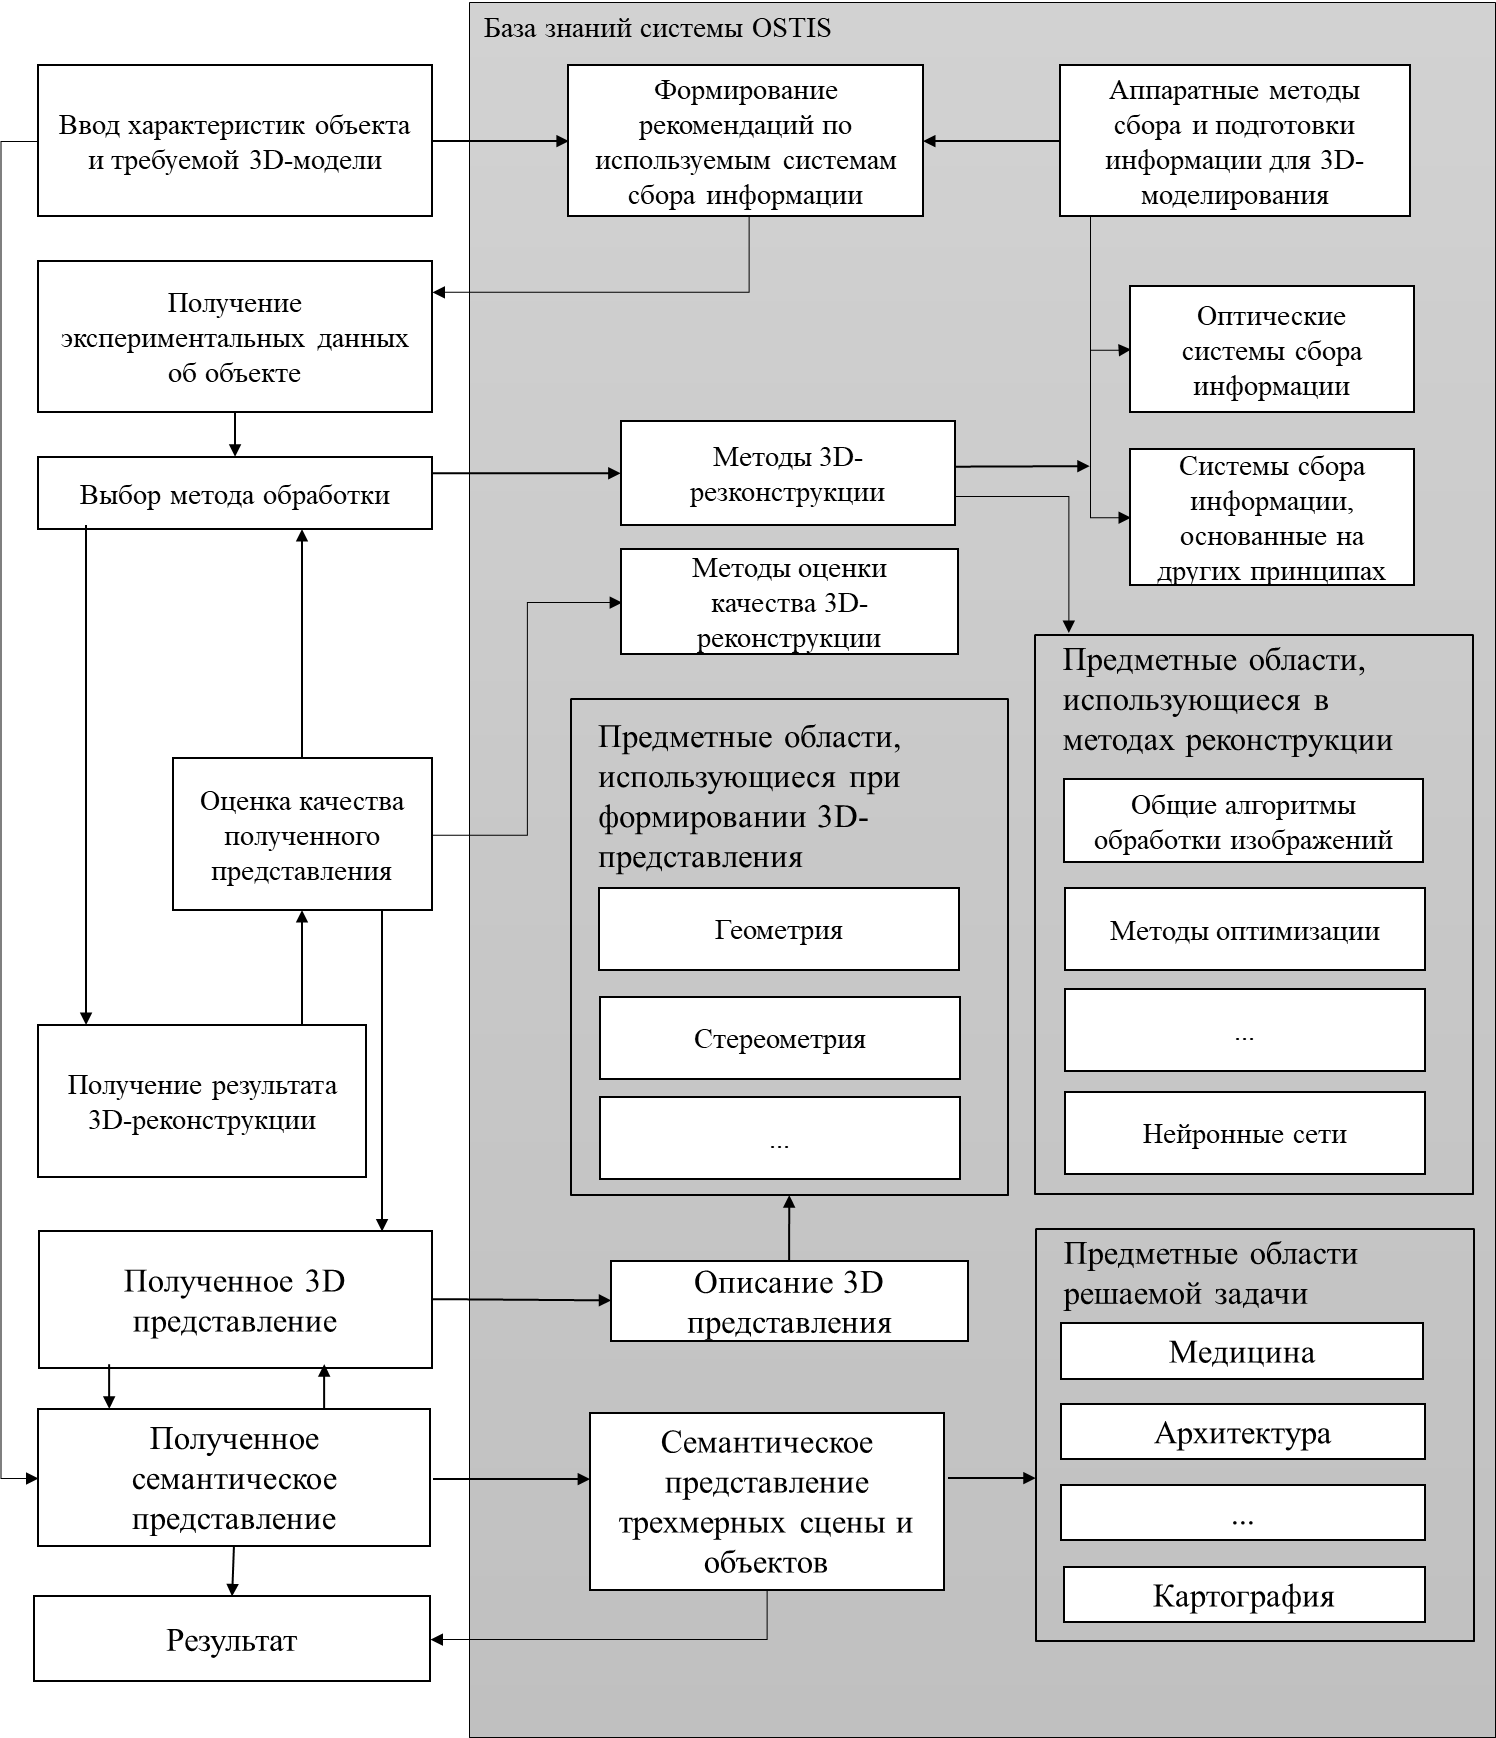
\includegraphics[scale=0.3]{author/part4/figures/schema3D.png}
    \label{fig:schema-3d-reconstruction}
\end{figure}

Далее более подробно рассмотрим основные указанные \textit{предметные области} и \textit{онтологии}.

\section{Семантическое представление объектов и сцены}
\label{sec_3d_models_semantics}

Важной составляющей \textit{интеллектуальных кибернетических систем}, использующих внутреннее \textit{трехмерное представление объектов}, является описание семантики этого представления. Информация об индивидуальных точках, поверхностях, полигонах или других примитивах не предоставляет информацию о смысловом наполнении этого представления --- точно так же, как отдельные буквы не позволяют оценить семантическую составляющую текстовых сообщений. \textit{ostis-система} предоставляет возможность формирования связанного семантического представления объекта, использующего дополнительную информацию из \textit{предметной области} рассматриваемого объекта.

В работе \scncite{Huang2023} продемонстрирована возможность использования такого комбинированного представления в задачах машинного обучения и распознавания образов. Данное представление также является основой для задач создания контента, в том числе основанных на генеративных состязательных нейросетевых моделях. Кроме этого, сопоставление пространственных и семантических свойств объекта способствует расширению функциональности и точности человеко-машинного взаимодействия в системах дополненной и виртуальной реальности, например, при проектировании обучающих или вспомогательных приложений (см. \scncite{Berestneva2022}, \scncite{Hervas2010}).

Семантическое описание объекта подразумевает ассоциацию множества точек, соответствующего некоторому объекту в трехмерном пространстве, с некоторым объектом имеющейся \textit{базы знаний}. Отношения в таких ассоциациях могут быть представлены в виде ``объект А представляет собой трехмерный образ некоторой сущности В'', где объект А задается внутренним \textit{трехмерным представлением объекта}, а сущность В --- некоторым описанием в \textit{базе знаний}.

Некоторые свойства сущности В, ассоциируемой с объектом А, могут быть естественным образом выведены из \textit{трехмерного представления этого объекта} --- в частности, информация о форме, свойствах поверхности, окраске и текстурировании может уже присутствовать в трехмерном описании. Таким образом, с помощью дополнительной обработки \textit{трехмерное представление объекта} А может являться источником фактологической информации о связанной сущности В. В то же время знание свойств сущности B может помочь при формировании более точного трехмерного образа объекта A. 

Аналогично семантическому описанию отдельного объекта может быть введено семантическое описание составных объектов. Следует иметь в виду, что семантическое наполнение индивидуальных составляющих не позволяет в полной мере определить семантику всего составного объекта целиком, поэтому аналогичную ассоциацию также необходимо задать и для всей совокупности. Например, объект ``велосипед'' может быть декомпозирован на составные объекты ``цепь'', ``рама'', ``колесо'' и так далее, однако набор семантических описаний \textit{трехмерных представлений объектов} составляющих по отдельности не позволяет формировать или учитывать семантику всего составного объекта целиком.

Семантическое описание части объекта должно содержать как информацию о базовом объекте, так и о дополнительном контексте относительно смыслового наполнения рассматриваемой части. Например, при видеоэндоскопическом анализе участка пищевода важной становится также информация о том, к какой именно части пищевода в организме относится этот участок.

Сцена представляет собой сложную композицию нескольких простых или составных объектов в некотором общем пространстве, дополненную данными об их взаимном расположении. Как и в случае с составными объектами, семантическое описание сцен должно включать не только описания индивидуальных составляющих, но и также смысловое наполнение эмержентных свойств всех этих составляющих в совокупности.

Таким образом, выделены следующие виды основных сущностей в рамках семантического представления сцен и объектов в \textit{трехмерном представлении}:

\begin{SCn}
    \scnheader{объект в трехмерном представлении}
    \scnidtf{множество точек в пространстве, соединенных между собой и имеющих одно смысловое представление}
\end{SCn}
\begin{SCn}
    \scnheader{составной объект в трехмерном представлении}
    \scnidtf{\textit{объект в трехмерном представлении}, подразумевающий декомпозицию на отдельные индивидуальные объекты}
\end{SCn}
\begin{SCn}
    \scnheader{часть объекта в трехмерном представлении}
    \scnidtf{множество точек в пространстве, принадлежащих некоторому \textit{объекту в трехмерном представлении}, которое может быть выделено по его геометрическому или смысловому представлению}
\end{SCn}
\begin{SCn}
    \scnheader{сцена в трехмерном представлении}
    \scnidtf{совокупность нескольких \textit{объектов в трехмерном представлении} и данных об их взаимном расположении в пространстве и свойствах, включающих абсолютные и относительные референтные ориентированные и неориентированные отношения}
\end{SCn}

Для \textit{сцены в трехмерном представлении} важными являются семантические характеристики визуального восприятия сцены с позиции некоторого помещенного в нее наблюдателя или \textit{системы компьютерного зрения}. В этом контексте сцена может быть представлена в виде отдельного наблюдения, например, двумерной проекции (или пары двумерных проекций в случае стереоскопического зрения). При этом семантика описаний исходных \textit{объектов в трехмерном представлении} и соответствующих им участков полученных проекций также может отличаться --- например, некоторые объекты могут находиться вне поля видимости, или восприниматься наблюдателем по-другому из-за наличия внешних факторов. К внешним факторам можно отнести наличие оптических, перспективных или психофизиологических эффектов (например, разница в освещении, оптическая дисторсия, различные иллюзии восприятия цвета или глубины, например, комната Эймса, и другие). 

Таким образом, важным является тот факт, что семантическое описание сцены должно включать как определение принадлежности индивидуальных объектов сцены некоторым сущностям имеющейся \textit{базы знаний}, так и описание возможных взаимосвязей между этими объектами, возникающих в силу их присутствия в сцене, или в силу их попарного взаимного расположения с позиции некоторого наблюдателя. Эта информация может естественным образом использоваться в качестве референтных свойств объектов сцены. Например, при наличии в сцене двух одинаковых объектов типа А и одного объекта типа В, некоторое логическое высказывание или запрос на естественном языке может использовать факт их взаимного расположения, например, для идентификации --- ``тот объект типа А, который находится слева от объекта типа Б''.


\begin{SCn}
    \scnheader{внешний фактор наблюдения сцены в трехмерном представлении}
    \scnidtf{параметр наблюдения \textit{сцены в трехмерном представлении}, определяющий пространственные, психофизические, визуальные и другие свойства восприятия системы наблюдения}
\end{SCn}
\begin{SCn}
    \scnheader{наблюдение сцены в трехмерном представлении}
    \scnidtf{описание \textit{сцены в трехмерном представлении} при фиксированном состоянии одного или \textit{нескольких внешних факторов наблюдения}. Может заключаться в понижении размерности представления информации, например, при приведении к двумерной проекции}
\end{SCn}
\begin{SCn}
    \scnheader{референтное отношение описания сцены в трехмерном представлении}
    \scnidtf{абсолютные и относительные ориентированные и неориентированные отношения отдельного \textit{наблюдения сцены в трехмерном представлении}}
\end{SCn}


Ниже приведены некоторые возможные \textit{референтные отношения описания сцены в трехмерном представлении} относительно различных \textit{внешних факторов наблюдения}. Следует отметить также, что в общем случае \textit{внешний фактор наблюдения} может быть задан произвольно соответствующей оценочной функцией, например, определения "схожести"{} объектов.

\begin{textitemize}
    \item информация о присутствии на сцене или проекции сцены:
    \begin{textitemize}
        \item объект отсутствует на сцене;
        \item объект присутствует, но не виден на проекции;
        \item объект присутствует и на проекции виден частично;
        \item объект присутствует и на проекции виден полностью;
    \end{textitemize}
    \item информация о взаимном расположении на проекции сцены:
    \begin{textitemize}
        \item по глубине:
        \begin{textitemize}
            \item за другим объектом;
            \item перед другим объектом;
        \end{textitemize}
    \end{textitemize}
    \begin{textitemize}
        \item по высоте:
        \begin{textitemize}
            \item выше другого объекта;
            \item на одном уровне с другим объектом;
            \item ниже другого объекта;
        \end{textitemize}
    \end{textitemize}
    \begin{textitemize}
        \item по расположению вдоль линии горизонта:
        \begin{textitemize}
            \item слева от другого объекта;
            \item справа от другого объекта;
        \end{textitemize}
    \end{textitemize}
    \item информация об относительном размере объектов на проекции:
    \begin{textitemize}
        \item больше другого объекта;
        \item одного размера с другим объектом;
        \item меньше другого объекта;
    \end{textitemize}
    \item информация о визуальном сходстве объектов:
    \begin{textitemize}
        \item похож или не похож на другой объект по форме;
        \item похож или не похож на другой объект по цвету;
        \item похож или не похож на другой объект по размеру.
    \end{textitemize}
\end{textitemize}


Пример описания \textit{сцены в трехмерном представлении}, включающий \textit{наблюдение сцены в трехмерном представлении} с точки зрения взаимного расположения объектов, представлен на рисунках \textit{\nameref{fig:scene-example}} и \textit{\nameref{fig:scene-description}}.

\begin{figure}[H]
    \caption{Рисунок. Пример трехмерной сцены, визуализированной в виде двумерной проекции с определенного положения камеры}
    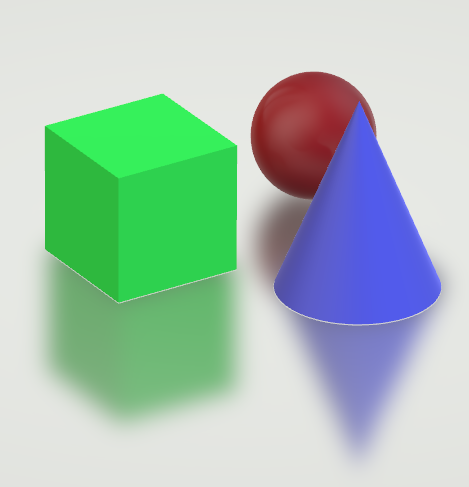
\includegraphics[scale=0.8, width=0.4\textwidth]{author/part4/figures/scene-example.png}
    \label{fig:scene-example}
\end{figure}

\begin{figure}[H]
    \caption{SCg-текст. Семантическое описание некоторых связей взаимного расположения объектов в сцене с положения наблюдателя}
    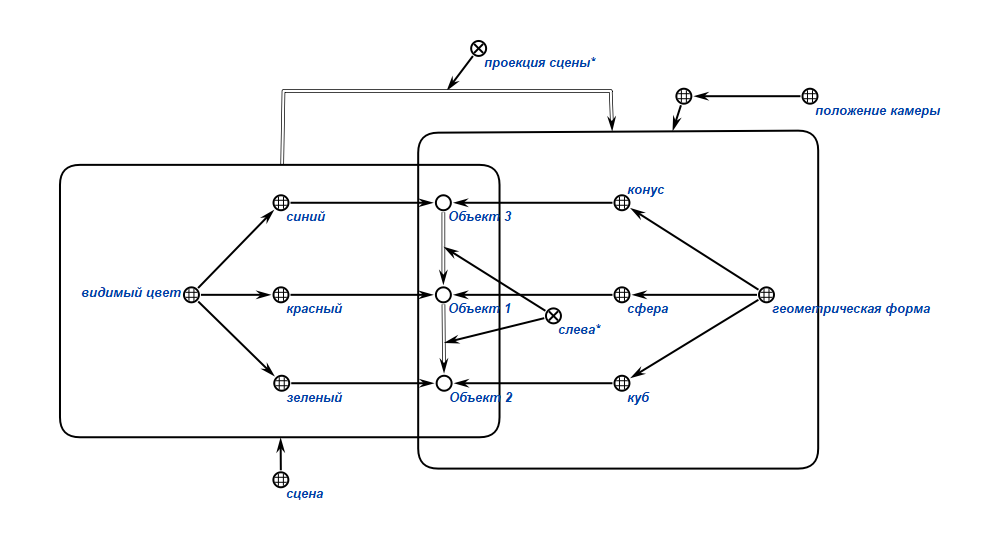
\includegraphics[scale=0.8, width=1.0\textwidth]{author/part4/figures/scene-description.png}
    \label{fig:scene-description}
\end{figure}

В данном случае семантическое описание \textit{сцены в трехмерном представлении} является совокупностью абсолютных и относительных характеристик, что позволяет задавать семантическое наполнение различным категориям высказываний. Допустим, объекты на рисунке имеют дополнительную визуальную характеристику цвета: зеленый куб, красная сфера, синий конус. Тогда для идентификации куба может быть приведено абсолютное описание свойства Объекта 2 ``видимый цвет'' --- ``зеленый'', но значение данного свойства может быть изменено при введении референтных отношений при таких внешних факторах как ``спектральный состав освещения'' или ``наличие у наблюдателя заболевания, связанного с цветовосприятием''. 

На рисунке приведено также референтное описание относительно внешнего фактора ``положение камеры'' --- ``куб слева от конуса'', выделяющее отдельное наблюдение сцены, представляющее собой в данном случае двумерную проекцию сцены. Структура \textit{сцены в трехмерном представлении}, основанная на описании присутствующих на этой сцене объектов, а также их свойств и \textit{референтных отношений} относительно \textit{внешнего фактора наблюдения} ложится в основу семантического описания сцены в большинстве задач \textit{компьютерного зрения}. Гранулярность и полнота семантического описания \textit{сцены в трехмерном представлении} определяется конкретной решаемой задачей. Использование такого описания открывает широкие возможности по организации \textit{пользовательского интерфейса}, поскольку предоставляет возможность выведения необходимого контекста для определения смыслового наполнения высказываний на \textit{естественном языке}. Кроме этого, такое представление может использоваться для генерации \textit{сцен в трехмерном представлении} и формирования интерактивных \textit{интерфейсов} взаимодействия с трехмерной средой.


\section{Трехмерное представление объектов в сцене}
\label{sec_3d_models_representation}

Как показано в предыдущем разделе системы позиционирования, распознавания и отображения объектов реального мира опираются не только на качественную составляющую описания, но и взаимное расположение объектов в пространстве или их отдельных частей. В соответствии с восприятием окружающего мира человеком \textbf{\textit{трехмерное представление объекта}} является наиболее информативным, хотя и необязательным. Полученные двумерные изображения, используемые во многих задачах, являются проекциями трехмерного пространства. Поэтому для рассматриваемых в данной главе задач максимальным классом объектов исследования выбрано \textit{трехмерное представление объектов}, включающее класс описаний, содержащих информацию о взаимном расположении объектов или их частей, заданных в трех координатах.

\begin{SCn}
    \scnheader{трехмерное представление объекта}
    \scnidtf{3D-представление объекта}
    \scnidtf{способ записи информации об объекте с сохранением его пространственных свойств в трех координатах}
    \begin{scnrelfromset}{разбиение}
        \scnitem{дискретное трехмерное представление}
        \scnidtf{трехмерное представление информации об объекте в виде дискретной совокупности трехмерных геометрических примитивов}
        \begin{scnrelfromset}{включает}
            \scnitem{воксельное представление}
            \scnidtf{представление в виде совокупности элементов, расположенных в регулярной сетке в трехмерном пространстве}
            \scnitem{облако точек}
            \scnidtf{трехмерное представление в виде неструктурированной совокупности точек}
            \scnitem{карта глубины}
            \scnidtf{двумерное изображение, на котором яркость пикселя определяет расстояние от плоскости изображения до соответствующей точки в пространстве}
        \end{scnrelfromset}
        \scnitem{поверхностное представление}
        \scnidtf{представление информации об объекте в виде совокупности поверхностей}
        \begin{scnrelfromset}{включает}
            \scnitem{аналитически задаваемая поверхность}
            \scnidtf{поверхность, заданная в трехмерном пространстве аналитически, например, уравнением}
            \scnitem{полигональная сетка}
            \scnidtf{совокупность вершин, ребер и граней, задающая некоторый многогранник в трехмерном пространстве}
            \scnitem{NURBS-поверхность}
            \scnidtf{поверхность, задаваемая с помощью совокупности неоднородных рациональных B-сплайнов через последовательность контрольных точек}
            \scnitem{поверхность разделения}
            \scnidtf{поверхность, образованная из полигональной сетки с помощью рекурсивного разделения граней этой сетки}
            \scnitem{поверхность на основе T-сплайнов}
            \scnidtf{модификация NURBS-поверхности, для которой последовательность контрольных точек может терминироваться без полного обхода всей поверхности}
        \end{scnrelfromset}
        \scnitem{специальные представления}
        \begin{scnrelfromset}{включает}
            \scnitem{видео 360}
            \scnidtf{видеопоследовательность, полученная с помощью захвата окружающего пространства во всех направлениях}
        \end{scnrelfromset}
    \end{scnrelfromset}
\end{SCn}

\begin{SCn}
    \scnheader{трехмерная модель объекта}
    \scnidtf{3D-модель объекта}
    \scnidtf{представление информации о конкретном объекте, записанное на основе одного из возможных трехмерных представлений}
\end{SCn}

Ниже даны определения некоторых терминов, относящихся к предметной области геометрии, стереометрии, функционального анализа и топологии, но необходимых для дополнения описания рассматриваемых видов \textit{трехмерного представления объектов}.

\begin{SCn}
    \scnheader{точка}
    \scnidtf{местоположение в пространстве, однозначно определяемое в системе координат}
\end{SCn}

\begin{SCn}
    \scnheader{геометрический примитив}
    \scnidtf{объект трехмерного пространства, который является атомарным (то есть непредставляемый в виде совокупности других объектов)}
\end{SCn}

\begin{SCn}
    \scnheader{вершина}
    \scnidtf{точка в трехмерном пространстве, задаваемая тремя координатами}
\end{SCn}

\begin{SCn}
    \scnheader{ребро}
    \scnidtf{отрезок между двумя вершинами}
\end{SCn}

\begin{SCn}
    \scnheader{грань}
    \scnidtf{замкнутая совокупность копланарных ребер}
\end{SCn}

\begin{SCn}
    \scnheader{полигон}
    \scnidtf{совокупность копланарных граней}
\end{SCn}

\begin{SCn}
    \scnheader{поверхность}
    \scnidtf{двумерное топологическое многообразие}
\end{SCn}

\begin{SCn}
    \scnheader{B-сплайн}
    \scnidtf{базисный сплайн}
    \scnidtf{сплайн-функция с наименьшим носителем для заданной степени порядка гладкости и разбиения области определения}
\end{SCn}


\section{Трехмерная реконструкция объектов окружающего мира}
\label{sec_3d_models_reconstruction}

Получить \textit{трехмерное представление объекта} на основе экспериментальных данных позволяет \textbf{\textit{трехмерная реконструкция}} объекта. \textit{Предметная область трехмерного представления объектов} затрагивает, как само описание объекта, так и методы его получения.

\begin{SCn}
    \scnheader{трехмерная реконструкция}
    \scnidtf{задача определения истинной формы объектов в \textit{трехмерном пространстве} на основании информации об этих объектах, получаемой в результате измерений, наблюдений или опытов}
\end{SCn}

Несмотря на то, что часть указанных выше задач требует дополнительных действий, все они основываются на получении \textit{трехмерного представления объекта}. В соответствии с этим каждая из задач также дополнительно может быть определена как внутренним состоянием, так и описанием условий, в рамках которых она осуществляется:
\begin{textitemize}
    \item описание цели --- тип \textit{трехмерного представления объекта}, разрешающая способность и точность;
    \item условия по возможности осуществления действий --- например, имеющееся оборудование или допустимое время выполнения;
    \item вид входных данных --- описание типа входного объекта.
\end{textitemize}

\textit{трехмерное представление объекта} или окружения, независимо от конкретного подкласса, может быть получено разными методами, в то же время конкретный метод может определять только одно представление.

\begin{SCn}
    \scnheader{методы трехмерной реконструкции}
    \begin{scnrelfromset}{включает}
        \scnitem{методы фотограмметрической реконструкции}
        \scnidtf{методы интерпретации изображений для определения \textit{трехмерного представления объекта} и его положения в пространстве по одной или нескольким фотографиям этого объекта}
        \begin{scnrelfromset}{подразделяется по взаимному положению объекта и камеры на}
            \scnitem{мобильные системы}
            \scnitem{макрофотограмметрия}
            \scnitem{спутниковая фотограмметрия}
            \scnitem{аэрофотограмметрия}
            \scnitem{наземная фотограмметрия}
            \scnitem{ближняя фотограмметрия}
        \end{scnrelfromset}
        \begin{scnrelfromset}{подразделяется по виду входной информации на}
            \scnitem{одно изображение}
            \scnitem{стерео изображения}
            \scnitem{многокадровые}
        \end{scnrelfromset}
        \scnitem{методы томографической реконструкции}
        \begin{scnrelfromset}{включает}
            \scnitem{реконструкция на основе Фурье-проекций }
            \scnitem{алгоритм обратной проекции}
            \scnitem{алгоритм итеративной реконструкции}
            \scnitem{реконструкция по коническому лучу}
            \scnitem{реконструкция на основе методов глубокого обучения }
        \end{scnrelfromset}
        \scnitem{методы структурированного подсвета}
        \begin{scnrelfromset}{включает}
            \scnitem{методы на основе световых сечений}
            \scnitem{методы на основе проекций полос}
            \scnitem{методы на основе фазового сдвига}
        \end{scnrelfromset}
        \scnitem{методы по оценке отраженного сигнала}
        \begin{scnrelfromset}{включает}
            \scnitem{измерение расстояния методами оптической модуляции}
            \scnitem{импульсная модуляция}
        \end{scnrelfromset}
        \scnitem{методы оценки по фокусировке}
        \begin{scnrelfromset}{включает}
            \scnitem{методы оценки из фокусировки}
            \scnitem{методы оценки из расфокусировки }
        \end{scnrelfromset}
        \scnitem{методы на основе теоремы о Фурье-проекциях}
        \scnitem{нейросетевые модели}
    \end{scnrelfromset}
\end{SCn}

Выше представлен один из вариантов онтологического описания \textit{методов} создания \textit{трехмерных представлений объектов}. Каждый из \textit{методов} \textit{трехмерной реконструкции} объектов в рамках этого описания может быть определен также кроме физического принципа его разрешающей способностью, типом входных данных, размером реконструируемых объектов и так далее. Полное описание представляет собой неиерархическую онтологическую структуру, строящуюся на основе \textit{базы знаний} \textit{ostis-системы}. Для дальнейшего взаимодействия агентов с данной структурой все эти описания ставятся в соответствие некоторым характеристикам. Характеристики могут относится как к отдельному методу, так и к группе методов, например, разрешающая способность может быть общей для всего подкласса электромагнитных волновых методов. Данные характеристики должны получаться агентами из самого представления знаний динамически, что позволяет дополнять и модифицировать общую структуру.
Для удобства представления данные характеристики можно выделить в спецификацию метода, на основании которой описывается область и возможность его применения. Она дает возможность использования методов для решения конкретных прикладных задач. В рамках спецификации (и, соответственно, структуры представления \textit{методов} в \textit{базе знаний}) задаются:
\begin{textitemize}
    \item тип возможных входных параметров;
    \item тип выходного представления --- в данном случае соответствующее трехмерное представление;
    \item время работы;
    \item разрешающая способность метода;
    \item расстояние от объекта до камеры;
    \item тип реконструируемого объекта;
    \item композиция сцены (отдельный объект, группа объектов, окружающее пространство);
    \item тип поверхности (глянцевость, прозрачность, цветность);
    \item наличие внутренней структуры;
    \item размер объекта.
\end{textitemize}

Описанная спецификация может быть интерпретируема промежуточным отношением для каждого метода. При наличии такого описания для промежуточных этапов данный подход позволяет проводить также комбинацию методов. Например, методы радиочастотного диапазона не дают возможность построить карту глубины, но позволяют получить положение камеры в глобальной системе координат в конкретный момент времени.

\section{Системы локального позиционирования, использующиеся в задачах трехмерной реконструкции}
\label{sec_3d_models_positioning}

В основе многих систем \textit{трехмерной реконструкции} лежит решение задачи локального позиционирования. Следует отметить, что в целом задача локального позиционирования является более общей, однако обычно рассматривается относительно наблюдателя, а не объекта.

\begin{SCn}
    \scnheader{система локального позиционирования}
    \scnidtf{автоматизированная система, обеспечивающая идентификацию, определение координат, отображение на плане местонахождения отдельных объектов или их частей в пределах территории, охваченной необходимой инфраструктурой}
\end{SCn}

Характеристики \textit{систем локального позиционирования}:
\begin{textitemize}
    \item точность позиционирования;
    \item достоверность позиционирования;
    \item периодичность опроса;
    \item надежность;
    \item габаритность.
\end{textitemize}

\begin{SCn}
    \scnheader{методы локального позиционирования}
    \begin{scnrelfromset}{включает}
        \scnitem{триангуляционные методы}
        \begin{scnindent}
            \scnidtf{методы, основанные на определении направления на источник сигнала}
            \scnitem{угол прихода сигнала}
            \begin{scnindent}
                \scnidtf{angle of arrival}
                \scnidtf{AoA}
                \scnidtf{направление, из которого принимается сигнал (например, радио, оптический или акустический)}
            \end{scnindent}
            \scnitem{угол вылета}
            \begin{scnindent}
                \scnidtf{angle of departure}
                \scnidtf{AoD}
                \scnidtf{направление, в котором отправляется сигнал (например, радио, оптический или акустический)}
            \end{scnindent}
        \end{scnindent}
        \scnitem{трилатерационные методы}
        \begin{scnindent}
            \scnidtf{методы, основанные на трилатерации, то есть на основе построения на местности смежных треугольников}
            \scnitem{время прибытия}
            \begin{scnindent}
                \scnidtf{time of arrival}
                \scnidtf{ToA}
                \scnidtf{абсолютный момент времени, когда радиосигнал, исходящий от передатчика, достигает удаленного приемника}
            \end{scnindent}
            \scnitem{разница во времени прибытия}
            \begin{scnindent}
                \scnidtf{time difference of arrival}
                \scnidtf{TDoA}
                \scnidtf{разница между временем прибытия сигнала до двух базовых станций}
            \end{scnindent}
            \scnitem{время полета}
            \begin{scnindent}
                \scnidtf{time of flight}
                \scnidtf{ToF}
                \scnidtf{время, затрачиваемое объектом, частицей или волной (акустической, электромагнитной и так далее) на преодоление расстояния через среду}
            \end{scnindent}
            \scnitem{двустороннее определение дальности}
            \begin{scnindent}
                \scnidtf{two-way ranging}
                \scnidtf{TWR}
                \scnidtf{метод определения дальности, который использует две задержки, которые обычно возникают при передаче сигнала, для определения дальности между двумя станциями: задержка распространения сигнала между двумя беспроводными устройствам, задержка обработки подтверждений в беспроводном устройстве}
            \end{scnindent}
            \scnitem{симметричное двустороннее определение дальности}
            \begin{scnindent}
                \scnidtf{symmetrical double-sided two-way ranging}
                \scnidtf{SDS TWR}
                \scnidtf{метод определения дальности, который использует двустороннее определение дальности дважды: относительно базовой станции и относительно мобильного устройства}
            \end{scnindent}
        \end{scnindent}
        \scnitem{методы на основе измерения силы сигнала}
        \begin{scnindent}
            \scnidtf{received signal strength indicator}
            \scnidtf{RSSI}
            \scnidtf{индикатор уровня мощности принимаемого сигнала. Данный метод позволяет определить местоположение устройства, основываясь на уровне силы сигнала, полученного базовой станцией или наоборот}
        \end{scnindent}
        \scnitem{одометрия}
        \begin{scnindent}
            \scnidtf{использование данных о движении приводов для оценки перемещения}
            \scnitem{визуальная одометрия}
        \end{scnindent}
    \end{scnrelfromset}
\end{SCn}

\begin{SCn}
    \scnheader{физические принципы позиционирования}
    \begin{scnrelfromset}{включает}
        \scnitem{акустические}
        \begin{scnindent}
            \scnidtf{основаны на использовании ультразвуковых (высокочастотных) звуковых волн}
        \end{scnindent}
        \scnitem{радиочастотные}
        \scnitem{магнитные}
        \begin{scnindent}
            \scnidtf{магнитный трекинг основан на измерении интенсивности магнитного поля в различных направлениях. Как правило, в таких системах есть базовая станция, которая генерирует переменное или постоянное магнитное поле}
        \end{scnindent}
        \scnitem{оптические}
        \begin{scnindent}
            \scnidtf{совокупность методов позиционирования на основе данных с камер видимого или инфракрасного диапазона}
            \scnitem{с внешней камерой}
            \scnitem{с внутренней камерой}
            \begin{scnindent}
                \scnitem{визуальная одометрия}
                \begin{scnindent}
                    \scnidtf{метод оценки положения и ориентации робота или иного устройства с помощью анализа последовательности изображений, снятых установленной на нем камерой (или камерами)}
                \end{scnindent}
            \end{scnindent}
            \scnitem{лазерное позиционирование}
            \begin{scnindent}
                \scnidtf{группа методов, основанных на оценке времени прохождения лазерных импульсов определенной периодичности}
            \end{scnindent}
        \end{scnindent}
        \scnitem{инерциальные}
        \begin{scnindent}
            \scnidtf{инерциальное позиционирование основано на свойствах инерции тел. Основная особенность этих методов состоит в том, что они не требуют внешних ориентиров или поступающих извне сигналов}
            \scnitem{гироскоп}
            \scnitem{акселерометр}
            \scnitem{магнитометр}
            \scnitem{барометр}
            \scnitem{гибридные}
        \end{scnindent}
    \end{scnrelfromset}
\end{SCn}

Описание и дальнейшее проектирование различных \textit{систем локального позиционирования} вызывает необходимость использования и других разделов \textit{базы знаний} \textit{ostis-системы}. 

\section{Базовые понятия компьютерного зрения в задаче трехмерной реконструкции}
\label{sec_3d_models_computervision}
\begin{SCn}
	\begin{scnrelfromlist}{подраздел}
		\scnitem{\ref{sec_3d_models_computervision_opt_systems}~\nameref{sec_3d_models_computervision_opt_systems}}
		\scnitem{\ref{sec_3d_models_computervision_local_features}~\nameref{sec_3d_models_computervision_local_features}}
	\end{scnrelfromlist}
\end{SCn}

\textit{компьютерное (техническое) зрение} как отдельная область исследований начала формироваться еще в 1960-х годах как попытка имитировать зрительную систему человека в робототехнике. Данное направление изначально основывалось на достижениях в области цифровой обработки изображений, однако в дальнейшем расширило перечень рассматриваемых задач, в том числе засчет попытки извлечения трехмерной структуры изображений с целью более полного понимания сцены. Понимание в этом контексте означает преобразование визуальных образов в описания мира, которые могут взаимодействовать с другими процессами и вызывать соответствующие действия. Считается, что в область \textit{компьютерного зрения} входят задачи распознавания образов, наблюдения, роботизированного управления, сегментации и интерпретации медицинских изображений, автоматического осмотра и сборки в заводских условиях, распознавания отпечатков пальцев и лиц, интерпретации жестов и многие другие (см. \scncite{Davies2021}).

\begin{SCn}
    \scnheader{компьютерное зрение}
    \scnidtf{техническое зрение}
    \scnidtf{междисциплинарная предметная область, описывающая совокупность технологий, методов и алгоритмов регистрации, обработки, анализа и получения символьного описания потоков данных с помощью различных источников визуальной информации, включая камеры видимого и инфракрасного спектра, трехмерные датчики и другие устройства визуализации, такие как компьютерные и магнитно-резонансные томографы.}
\end{SCn}

\subsection{Оптические системы компьютерного зрения}
\label{sec_3d_models_computervision_opt_systems}

В области \textit{трехмерной реконструкции} используются системы, регистрирующие излучение в различных диапазонах длин волн --- от рентгеновского (рентгеновский сканер) до радиоволнового (электромагнитная катушка). Наиболее распространенным подходом для анализа является использование излучения в видимом диапазоне (380 нм --- 720 нм), регистрируемого \textit{оптической системой компьютерного зрения}, например, камерой (фотоаппаратом). 

\begin{SCn}
    \scnheader{оптическая система компьютерного зрения}
    \scnidtf{совокупность оптических элементов, обеспечивающая регистрацию электромагнитного поля видимого, ультразвукового и инфракрасного диапазона с целью дальнейшей обработки и получения количественного и символьного описания информации.}
\end{SCn}

Одним из наиболее распространенных видов \textit{оптической системы компьютерного зрения} для регистрации информации об объекте является цифровая камера. При использовании цифровой камеры формой представления полученных данных является снимок, который может быть представлен в виде растрового изображения. При этом в контексте конкретной рассматриваемой задачи важными могут являться не только параметры полученного изображения, но и фиксация условий проведения съемки и параметров \textit{оптической системы компьютерного зрения}.  

Изображение является двумерной проекцией исходного трехмерного пространства. \textit{трехмерную модель} рассматриваемого объекта по нескольким снимкам или видеоряду можно получить на основе восстановления параметров проекций, связанных с каждым из снимков, и выстраиванием этих проекций в одном трехмерном пространстве. При наличии пересекающихся лучей, направленных в одну и ту же точку реального объекта, по проекциям можно восстановить параметры объекта и сцены в связанной с этим пространством системе координат. По схожему принципу устроена зрительная система человека, основанная на анализе разницы между изображениями, получаемыми левым и правым глазом, а также последовательно полученными изображениями на сетчатке одного глаза в небольшом временном диапазоне.

\begin{SCn}
    \scnheader{проекция}
    \scnidtf{отображение точек, фигур, векторов пространства любой размерности на его подпространство любой размерности}
\end{SCn}

\begin{SCn}
    \scnheader{бинокулярное зрение}
    \scnidtf{способность одновременно четко видеть изображение предмета обоими глазами; в этом случае человек видит одно изображение предмета, на который смотрит}
\end{SCn}

\begin{SCn}
    \scnheader{стереоскопическое зрение}
    \scnidtf{вид зрения, при котором возможно восприятие формы, размеров и расстояния до предмета, благодаря восприятию двух изображений, полученных в пределах бесконечно малого промежутка времени при разных параметрах внешнего ориентирования оптической системы в пространстве}
\end{SCn}

Для описания преобразования между объектами в исходном трехмерном пространстве и их проекцией используется модель проекции. Модель проекции при использовании в системах \textit{трехмерной реконструкции} описывает ход световых лучей в \textit{оптической системе компьютерного зрения} и относится к области изучения эпиполярной геометрии. Наиболее известной, использующейся в геометрии является модель ортогональной проекции. Но для работы с \textit{оптическими системами компьютерного зрения} больше подходит модель центральной проекции, которая описывает ход лучей в камере-обскуре. \textit{оптическую систему компьютерного зрения} можно считать аналогичной камере-обскуре, если она содержит симметричную систему линз и не вносит криволинейных искажений, то есть все прямые исходной трехмерной сцены остаются прямыми и не искривляются после проекции. В общем случае модель проекции может учитывать различные особенности \textit{оптической системы компьютерного зрения} или среды получения изображения. Например, в работе \scncite{Halavataya2019} предлагается модель широкоугольной сферической проекции, учитывающая дисторсионные искажения, вызываемые широкоугольной камерой. Использование корректной модели проекции напрямую влияет на качество реконструируемых трехмерных сцен и объектов.

\begin{SCn}
    \scnheader{эпиполярная геометрия}
    \scnidtf{один из подразделов оптики, который занимается геометрической интерпретацией формирования двумерных изображений по трехмерной сцене. Чаще всего в этом контексте рассматривается задача геометрических преобразований лучей света, которые отражаются от наблюдаемой трехмерной сцены, улавливаются некоторой \textit{оптической системой компьютерного зрения} и проецируются на фоточувствительную двумерную поверхность (например, пленку или цифровую матрицу) для формирования изображения}
\end{SCn}

\begin{SCn}
    \scnheader{модель проекции}
    \scnidtf{математическая модель, в соответствии с которой осуществляется построение проекции}
    \begin{scnrelfromset}{включает}
        \scnitem{параллельная проекция}
        \scnidtf{вид проекции, при котором проецирующиеся лучи строятся параллельными друг другу}
        \begin{scnindent}    
            \scnitem{ортогональная проекция}
            \scnidtf{вид параллельной проекции, в которой проецирующие лучи строятся перпендикулярно некоторой заданной плоскости, например, плоскости изображения}
        \end{scnindent}
        \scnitem{центральная проекция}
        \scnidtf{вид проекции, при котором все прямые, построенные на проецирующихся лучах, пересекаются в одной точке, называемой центром проекции. Параллельная проекция может считаться предельным случаем центральной проекции с центром проекции, удаленным на бесконечное расстояние}
    \end{scnrelfromset}
\end{SCn}

Для полного задания модели проекции вводятся параметры, называемые параметрами ориентирования, однозначно характеризующие положение снимка относительно некоторой глобальной системы координат. Выделяют параметры внутреннего и внешнего ориентирования. Параметры внутреннего ориентирования задают относительное положение точки фотографирования и самого снимка. В модели центральной проекции к параметрам внутреннего ориентирования относятся 3 величины: двумерные координаты главной точки снимка $(x_0,y_0)$ и фокусное расстояние $f$. К параметрам внешнего ориентирования относят 6 величин, задающих связь проецирующих лучей в момент съемки с глобальной системой координат: координаты точки положения камеры $(x_C,y_C,z_C)$, два угла, определяющие положение главного луча камеры $(\omega,\varphi)$ и угол поворота снимка $\beta$. Для перехода в новое пространство необходимо осуществить пространственное преобразование между системами координат. Для этого используется преобразование Гельмерта, зависящее от 7 параметров: координаты начала системы координат снимка xyz в глобальной координатной системе OXYZ $(X_0,Y_0,Z_0)$, три угла поворота $(\omega,\varphi, \beta)$ относительно осей $X$,$Y$,$Z$ и коэффициент масштаба $m$. На основании данных углов можно построить матрицу поворота, задающую преобразование координат из одной системы в другую при последовательном повороте вокруг каждой из осей.

\begin{SCn}
    \scnheader{параметры ориентирования модели центральной проекции}
    \scnidtf{параметры, задающие связь координат объекта на изображении и в трехмерном пространстве при условии, что ход лучей и, соответственно, формирование изображения в \textit{оптической системе компьютерного зрения} описывается центральной проекцией }
    \begin{scnrelfromset}{включает}
        \scnitem{параметры внутреннего ориентирования}
        \begin{scnrelfromset}{включает}
            \scnitem{фокусное расстояние}
            \scnitem{координаты главной точки снимка ($x_0$, $y_0$)}
        \end{scnrelfromset}
        \scnitem{параметры внешнего ориентирования}
        \begin{scnrelfromset}{включает}
            \scnitem{координаты точки положения камеры ($x_C$, $y_C$, $z_C$)}
            \scnitem{углы, определяющие положение главного луча камеры $(\omega,\varphi)$}
            \scnitem{угол поворота снимка $\beta$}
        \end{scnrelfromset}
    \end{scnrelfromset}
\end{SCn}

\begin{SCn}
    \scnheader{калибровка камеры}
    \scnidtf{задача получения внутренних и внешних параметров камеры по имеющимся фотографиям или видео, отснятыми ею}
\end{SCn}

Калибровка камеры часто используется на начальном этапе решения многих задач \textit{компьютерного зрения} и, в особенности, задач, связанных с дополненной реальностью. Кроме того, калибровка камеры может использоваться для исправления искажений, вызванных \textit{оптической системой компьютерного зрения}, например, дисторсии.

\begin{SCn}
    \scnheader{оптическая аберрация}
    \scnidtf{отклонение от идеальной модели формирования изображения в оптической системе}
\end{SCn}

\begin{SCn}
    \scnheader{дисторсия}
    \scnidtf{аберрация оптических систем, при которой коэффициент линейного увеличения изменяется по мере удаления отображаемых предметов от оптической оси}
    \begin{scnrelfromset}{включает}
        \scnitem{радиальная дисторсия}
        \scnidtf{дисторсия, вызванная сферической поверхностью линз оптической системы}
        \scnitem{тангенциальная дисторсия}
        \scnidtf{дисторсия, вызванная неперпендикулярностью главной оптической оси и плоскости изображения и прохождением главной оптической оси не через центр снимка}
    \end{scnrelfromset}
\end{SCn}

\subsection{Локальные признаки изображений}
\label{sec_3d_models_computervision_local_features}

Одним из первых этапов \textit{трехмерной реконструкции} по изображениям, полученным с различных ракурсов, является нахождение всевозможных комбинаций соответствующих точек на изображениях, которые являются одной и той же точкой исходной сцены. Традиционно для решения этой задачи используются алгоритмы для работы с \textit{локальными признаками изображения}.

\begin{SCn}
    \scnheader{локальный признак изображения}
    \scnidtf{некоторое подмножество точек изображения, пространственные окрестности которых определенным образом характеризуют изображение целиком или присутствующие на нем объекты}
    \begin{scnrelfromset}{включает}
        \scnitem{ключевая точка}
    \end{scnrelfromset}
\end{SCn}

Основной сложностью при реализации и работе с алгоритмами нахождения \textit{локальных признаков изображения} является тот факт, что универсального или однозначно точного определения того, что именно является локальным признаком, не существует. Конкретное определение \textit{локального признака} в произвольной точке произвольного изображения зависит от вида используемого алгоритма и решаемой задачи. К основным концепциям, на основании которых принимается решение о наличии в точке \textit{локального признака изображения}, в различных исследованиях относят модуль и направление градиента, определяемые по разностной схеме значения лапласиана или гессиана в окрестности точки, собственные значения и векторы и тому подобные. В работе {\scncite{Krig2016}} приводится таксономия атрибутов описательных характеристик \textit{локальных признаков изображения} для их более высокоуровневого анализа. Алгоритмы детектирования \textit{локальных признаков изображения}, как правило, являются входной точкой для последующей обработки другими методами. Методы глубкого обучения, такие как сверточные нейронные сети, также основаны на выделении низкоуровневневых \textit{локальных признаков изображения} с помощью операции свертки.

В задачах \textit{трехмерной реконструкции} основной интерес представляет не само нахождения \textit{локальных признаков изображения}, а их сопоставление между несколькими кадрами для нахождения смещения объектов. Зная параметры \textit{оптической системы компьютерного зрения} в момент получения каждого снимка и сопоставив смещение объектов на отдельных изображениях, можно получить расстояние между объектами в глобальной системе координат. Поэтому базовой задачей является построение карты диспарантности.

\begin{SCn}
    \scnheader{диспарантность}
    \scnidtf{различие взаимного положения двух точек, отображаемых на двух изображениях и соответствующих одной точке пространства}
\end{SCn}

\begin{SCn}
    \scnheader{карта диспарантности}
    \scnidtf{набор значений, соответстветствующих пикселям исходного изображения и отображающих смещение каждого исходного пикселя относительно его положения на другом изображении. Чаще всего отображается также в виде изображения, при этом значение яркости пикселей отражает величину смещения}
\end{SCn}

Карты диспарантности могут быть получены различными методами, основанными как на статистических характеристиках отдельных областей изображений, так и на нахождении ключевых точек и сопоставлении их на основе некоторого описания окрестности (то есть значения, полученного с помощью алгоритма дескриптора). Во втором случае карта диспарантности может быть построена не для всего изображения, а только для подмножества пикселей, соответствующих ключевым точкам. Данный подход является одним из основных этапов методов \textit{фотограмметрической реконструкции}, включающим нахождение всевозможных комбинаций соответствующих точек на изображениях проекций, которые относятся к одной и той же точке исходной сцены.

\begin{SCn}
    \scnheader{методы построения карты диспарантности}
    \begin{scnrelfromset}{включает}
        \scnitem{вычисление суммы абсолютных разностей для небольших окрестностей изображения}
        \scnitem{вычисление суммы квадратов разностей для небольших окрестностей изображения}
        \scnitem{вычисление нормализованной кросскорреляции для небольших окрестностей изображений}
        \scnitem{нейросетевые алгоритмы для вычисления карты диспарантности}
        \scnitem{детекторы и дескрипторы ключевых точек}
        \begin{scnindent}
            \scnitem{детекторы}
            \begin{scnindent}
                \scnidtf{алгоритмы, которые по входному изображению генерируют набор ключевых точек}
                \scnitem{эмпирические детекторы}
                \begin{scnindent}
                    \scnidtf{алгоритмы поиска ключевых точек, которые основаны на некоторых интуитивных представлениях, практическом опыте и результатах тестирования}
                    \scnitem{FAST (см. \scncite{Rosten2006})}
                    \scnitem{детектор Харриса (см. \scncite{Harris1988})}
                    \scnitem{SUSAN (см. \scncite{Smith1997})}
                \end{scnindent}
                \scnitem{статистические детекторы}
                \begin{scnindent}
                    \scnidtf{алгоритмы поиска ключевых точек, которые основаны на сравнении статистических характеристик точки или ее окрестности с некоторыми заранее известными}
                    \scnitem{SIFT (см. \scncite{Lowe2004})}
                    \scnitem{AGAST (см. \scncite{Mair2010})}
                \end{scnindent}
                \scnitem{детекторы на основе машинного обучения}
                \begin{scnindent}
                    \scnidtf{алгоритмы поиска ключевых точек, которые основаны, как правило, на существующих эмпирических или статистических детекторах, но использующие оптимизацию некоторых варьируемых параметров детектирования методами машинного обучения}
                    \scnitem{FAST-ER (см. \scncite{Rosten2010})}
                    \scnitem{TILDE (см. \scncite{Verdie2015})}
                \end{scnindent}
            \end{scnindent}
            \scnitem{дескрипторы}
            \begin{scnindent}
                \scnidtf{алгоритмы, которые по входному изображению и набору координат точек на них, генерируют вектор признаков, описывающий эти точки в некотором метрическом пространстве}
                \scnitem{гистограммные дескрипторы}
                \begin{scnindent}
                    \scnidtf{алгоритмы, строящие вектор представления для описания ключевой точки на основании гистограммы некоторой статистики, которую можно вычислить по ее окрестности. Вектора описаний гистограммных дескрипторов обычно имеют размерность не менее 128, значения отдельных элементов являются вещественными числами, так как гистограмма, как правило, нормализуется}
                    \scnitem{SIFT (см. \scncite{Lowe2004})}
                    \scnitem{SURF (см. \scncite{Bay2008})}
                \end{scnindent}
                \scnitem{бинарные дескрипторы}
                \begin{scnindent}
                    \scnidtf{алгоритмы, разработанные с целью ускорения сопоставления векторов описаний точек и строящие вектор представления для описания ключевой точки, состоящий из элементов булева множества}
                    \scnitem{BRIEF (см. \scncite{Calonder2010})}
                    \scnitem{ORB (см. \scncite{Rublee2011})}
                    \scnitem{BRISK (см. \scncite{Leutenegger2011})}
                \end{scnindent}
            \end{scnindent}
        \end{scnindent}
        \scnitem{методы оптического потока}
        \begin{scnindent}
            \scnidtf{методы отображения видимого движения объектов, поверхностей или краев сцены, получаемых в результате относительного перемещения наблюдателя и объектов сцены}
            \scnitem{фазовая корреляция}
            \begin{scnindent}
                \scnidtf{методы оптического потока, основанные на инверсии нормализованного перекрестного спектра}
            \end{scnindent}
            \scnitem{блочные методы}
            \begin{scnindent}
                \scnidtf{методы оптического потока, основанные на минимизации суммы квадратов или суммы модулей разностей}
            \end{scnindent}
            \scnitem{дифференциальные методы оценки оптического потока, основанные на частных производных сигнала}
            \begin{scnindent}
                \scnitem{алгоритм Лукаса-Канаде (см. \scncite{Lucas1981})}
                \scnitem{Horn-Schunck (см. \scncite{Horn1981})}
                \begin{scnindent}
                    \scnidtf{алгоритмы, основанные на минимизации функционала, описывающего отклонение от предположения о постоянстве яркости и гладкости получаемого векторного поля}
                \end{scnindent}
                \scnitem{общие вариационные методы}
                \begin{scnindent}
                    \scnidtf{методы, основанные на модификации метода Horn-Schunck, но использующие другие ограничения на данные и другие ограничения на гладкость}
                \end{scnindent}
            \end{scnindent}
            \scnitem{дискретные методы оптимизации}
            \begin{scnindent}
                \scnidtf{методы, основанные на квантовании поискового пространства и присвоении каждому пикселю изображения метки таким образом, чтобы расстояние между последовательными кадрами было минимальным}
            \end{scnindent}
        \end{scnindent}
    \end{scnrelfromset}
\end{SCn}

Количество и распределение выделенных \textit{локальных признаков изображения} влияет на возможность не только проведения \textit{трехмерной реконструкции}, но и на качество результатов других задач \textit{компьютерного зрения}. При этом как не существует точного определения, что должен представлять \textit{локальный признак изображения}, так и не существует универсального алгоритма, позволяющего работать с любым видом изображений. В работе \scncite{Halavataya2020} приведены примеры параметров изображения, на основании которых могут подбираться соответствующие параметры алгоритмов детекторов и дескрипторов ключевых точек. Данные параметры также могут быть описаны в рамках \textit{базы знаний} \textit{ostis-системы}, что позволит построить адаптивную систему подбора алгоритма выделения \textit{локальных признаков изображения} в связанных задачах \textit{компьютерного зрения}.

\section{Онтология действий, выполняемых в предметной области трехмерной реконструкции}
\label{sec_3d_models_actions}
\begin{SCn}
\begin{scnrelfromlist}{подраздел}
    \scnitem{\ref{sec_3d_models_actions_interm}~\nameref{sec_3d_models_actions_interm}}
    \scnitem{\ref{sec_3d_models_actions_final}~\nameref{sec_3d_models_actions_final}}
    \scnitem{\ref{sec_3d_models_actions_gen}~\nameref{sec_3d_models_actions_gen}}
\end{scnrelfromlist}
\end{SCn}
На верхнем уровне любой метод \textit{трехмерной реконструкции} может быть представлен в виде процедурного знания, например, в виде последовательности этапов, в соответствии с которыми входные данные для \textit{трехмерной реконструкции} преобразовываются в итоговое \textit{трехмерное представление объекта}.

Общая черта многих методов \textit{трехмерной реконструкции} --- использование промежуточного (или конечного) представления об объектах окружающего мира в трех координатах. Другими словами, метод \textit{трехмерной реконструкции} можно представить в виде последовательности действий по формированию набора элементов, характеризующихся координатами в общем трехмерном пространстве, которые в дальнейшем, при необходимости, могут быть достроены до поверхностей, скомбинированы с двумерными представлениями и так далее для формирования нужного выходного представления:

\begin{equation}
    r:I{m(R^3)}\rightarrow O
\end{equation}

где I --- входные данные, $R^3$ --- общее трехмерное декартово пространство, $m(R^3)$ --- описание элемента в системе координат общего трехмерного пространства, $O$ --- выходное \textit{трехмерное представление объекта}. Чаще всего в качестве элементов промежуточного представления выступают отдельные точки трехмерного пространства --- в этом случае такое представление называют облаком точек.

В качестве элементов могут также выступать отрезки кривых, аналитически задаваемые поверхности, полигоны и другие виды объектов.

В качестве источников данных о трехмерных координатах для промежуточного представления могут выступать:
\begin{textitemize}
    \item Непосредственно абсолютные значения трехмерных координат точек, то есть в этом случае входные данные $I$ представляют собой набор точек ${R^3}$. Это характерно для всех методов, которые позволяют строить карту глубины сцены, так как представление в виде карты глубины с известными координатами положения наблюдателя и фокусного расстояния карты позволяет определить трехмерные координаты любой точки на ней.
    \item Данные, по которым с помощью некоторой дополнительной обработки могут быть получены значения трехмерных координат отдельных точек. Такие представления, как правило, намного более распространены и просты в получении.
\end{textitemize}

Следует отметить, что различные источники данных при формировании промежуточного представления могут использоваться совместно, при наличии у каждого из источников некоторой привязки к общей системе координат.

Как для получения промежуточного \textit{трехмерного представления объекта}, так и для формирования на его основе итогового представления могут использоваться различные методы и алгоритмы, структура и взаимосвязь которых определяют итоговую последовательность действий по выполнению \textit{трехмерной реконструкции} объекта или сцены.


\subsection{Действия по формированию промежуточного трехмерного представления}
\label{sec_3d_models_actions_interm}

Многие методы дистанционного зондирования полагаются на наличие априорной информации о трехмерных координатах исследуемого объекта, по которой можно построить облако точек для промежуточного \textit{трехмерного представления объекта}. К таким относятся методы, которые позволяют оценивать расстояние от измерительного прибора до объекта. Тем не менее, использование этих методов требует более сложного оборудования, применение которого может быть затруднено в некоторых сценариях.

В этой связи, в качестве отдельной категории методов исследования можно выделить группу методов формирования промежуточного представления в виде облака точек по более традиционным видам информации. К таким относятся методы генерации по одному изображению, стереопаре, набору изображений или видеоряду, в которых также может использоваться информация об \textit{оптической системе компьютерного зрения}, которая была использована для получения изображения.

Таким образом можно выделить следующие виды входных данных:
\begin{textitemize}
    \item статическое изображение или набор статических изображений;
    \item видеоряд (набор статических изображений с временной меткой);
    \item стереопара (2 статических изображения с параметрами \textit{оптической системы компьютерного зрения}) или набор стереопар;
    \item стерео-видеоряд (набор стереопар с временной меткой);
    \item информация об \textit{оптической системе компьютерного зрения}.
\end{textitemize}

В качестве выходного представления в данном случае выступает разреженное облако точек \textit{трехмерного пространства}, с привязкой каждой из точек этого пространства к одной или нескольким точкам исходных входных изображений.

Формирование разреженного облака точек включает в себя следующие этапы, для каждого из которых могут быть определены указанные параметры:
\begin{textitemize}
    \item предобработка;
    \item нахождение \textit{локальных признаков изображения} (обычно заключается в детектировании ключевых точек):
    \begin{textitemize}
        \item алгоритм-детектор;
    \end{textitemize}
    \item cопоставление ключевых точек:
    \begin{textitemize}
        \item алгоритм-дескриптор или алгоритм оптического потока;
        \item прореживание;
    \end{textitemize}
    \item оценка положений камеры:
    \begin{textitemize}
        \item модель проекции;
        \item алгоритм оценки связок;
    \end{textitemize}
    \item постобработка.
\end{textitemize}

Детектирование и сопоставление ключевых точек позволяет определить точки, принадлежащие одному и тому же объекту исследуемого трехмерного пространства, при наличии достаточного количества изображений. На этапе оценки положения камеры используется математическая модель проекции, задающая взаимосвязь между двумерными координатами точки на изображении и соответствующими ей трехмерными координатами в пространстве моделирования; на этом же этапе может осуществляться эмпирическая оценка глубины, например, при помощи \textit{нейросетевых методов}. Каждое соответствие, описанное математически с помощью модели проекции, в дальнейшем используется в алгоритме оценки связок для того, чтобы восстановить в трехмерном пространстве положения камеры для каждого из исследуемых изображений, а также определить расстояния от камер до точек, исходя из некоторого критерия минимизации ошибки обратной проекции.

Например, классический метод \textit{трехмерной реконструкции} \textit{Structure from Motion} по нескольким входным изображениям в рамках представленного конвейера можно описать следующими характеристиками:
\begin{textitemize}
    \item предобработка --- преобразование к оттенкам серого;
    \item алгоритм-детектор --- SIFT, SURF, FAST;
    \item алгоритм-дескриптор --- SIFT, SURF, ORB;
    \item прореживание --- RANSAC;
    \item модель проекции --- центральная проекция;
    \item алгоритм оценки связок --- глобальный метод связок с оптимизацией методом Левенберга-Марквардта.
\end{textitemize}
В качестве еще одного примера рассмотрим метод одновременной локализации и построения карты ORB-SLAM, использующий в качестве входного представления видеоряд:
\begin{textitemize}
    \item предобработка --- прореживание кадров;
    \item алгоритм-детектор --- FAST;
    \item алгоритм-дескриптор --- ORB + метод оптического потока Лукаса-Канаде;
    \item прореживание --- RANSAC, прореживание по инвариантам движения;
    \item модель проекции --- центральная проекция;
    \item алгоритм оценки связок --- инкрементальный метод связок с фиксированным положением камеры и фиксированным положением ключевых точек между кадрами, метод построения карты по движению;
    \item постобработка --- уточнение траектории и детектирование петель.
\end{textitemize}

Онтологическое описание представленной последовательности действий, а также пример конкретного алгоритма, реализованного по этой последовательности действий в рамках \textit{ostis-системы}, представлены на рисунках \textit{\nameref{fig:reconstruction}} и \textit{\nameref{fig:reconstruction-example}}.

\begin{figure}[H]
    \caption{SCg-текст. Онтологическое описание последовательности действий по построению промежуточного \textit{трехмерного представления} в виде разреженного облака точек}
    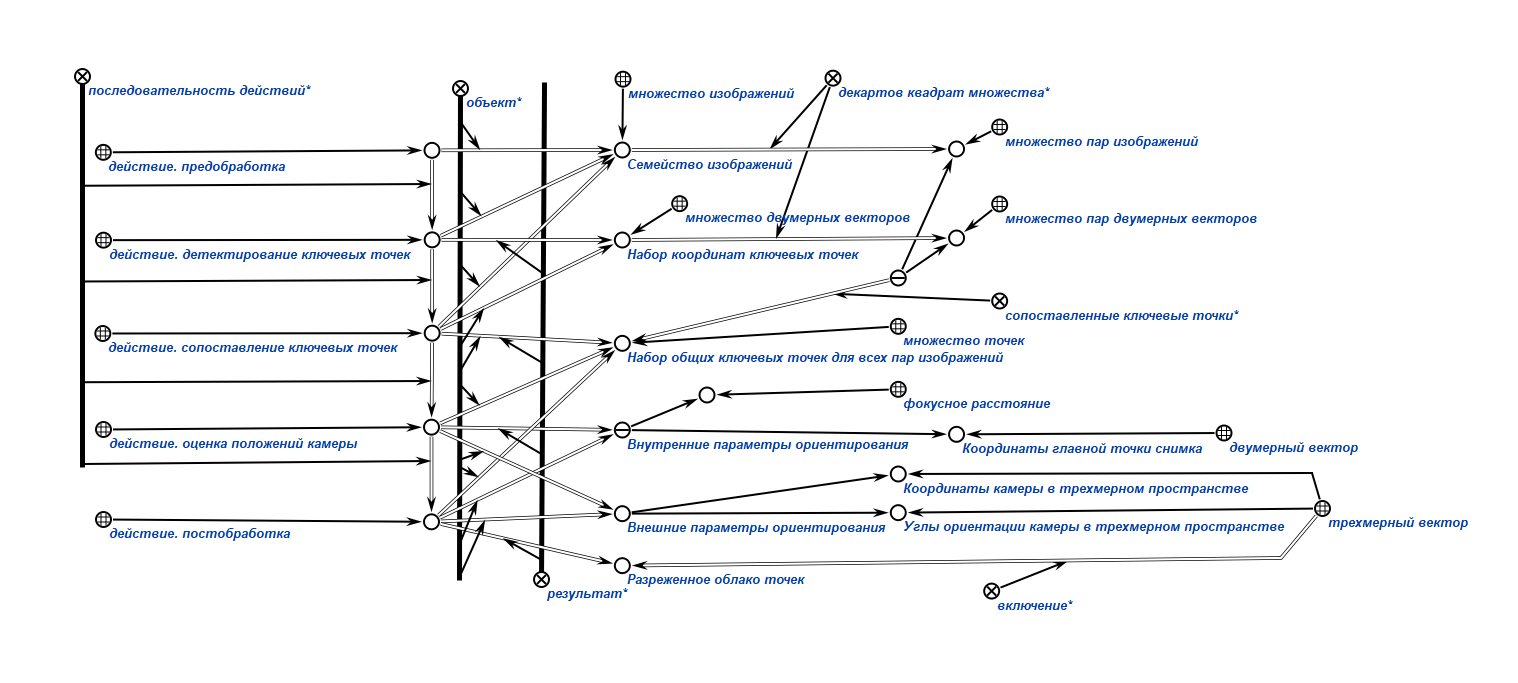
\includegraphics[scale=0.8, width=1.0\textwidth]{author/part4/figures/reconstruction.png}
    \label{fig:reconstruction}
\end{figure}

\begin{figure}[H]
    \caption{SCg-текст. Пример алгоритма построения разреженного облака точек на основе представленного описания}
    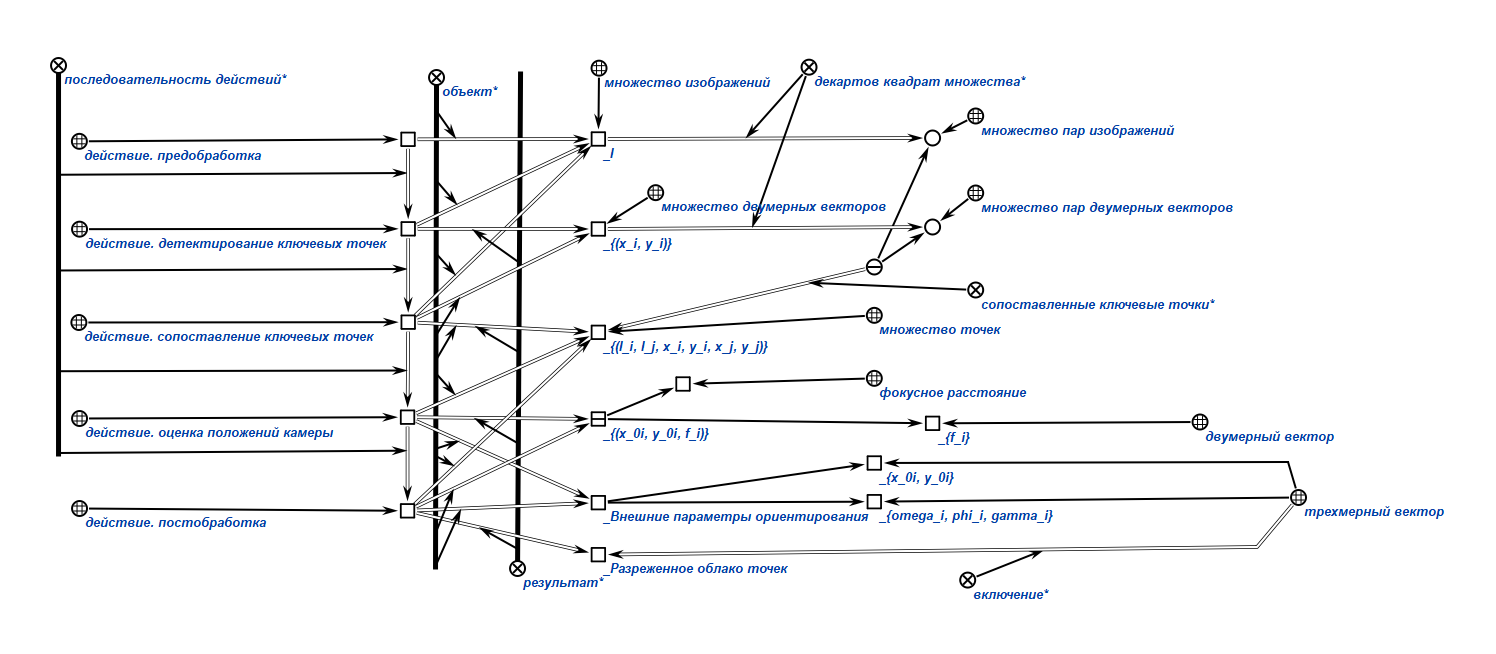
\includegraphics[scale=0.8, width=1.0\textwidth]{author/part4/figures/reconstruction-example.png}
    \label{fig:reconstruction-example}
\end{figure}

Поскольку каждый из предложенных этапов описан в виде функционального отображения, предполагается добавление, удаление или модификация этапов при обработке, если соблюдается соответствие типов входных и выходных представлений в контексте решаемой задачи.

\subsection{Действия по формированию итогового трехмерного представления}
\label{sec_3d_models_actions_final}

В некоторых задачах разреженное облако точек в трехмерном пространстве может выступать достаточным представлением, и может считаться итогом работы алгоритма \textit{трехмерной реконструкции}. Также достаточно популярным является представление в виде уплотненного цветного облака точек.

Тем не менее, во многих задачах такого представления недостаточно, поэтому можно выделить класс действий при формировании более сложного \textit{трехмерного представления объекта}, в зависимости от типа требуемого выходного представления. В качестве входного представления для этого этапа выступает разреженное облако точек, а также дополнительная информация о связи конкретных точек облака с исходными представлениями.

Описание методов формирования итогового \textit{трехмерного представления объекта} можно представить в виде совокупностей следующих этапов, с соответствующими параметрами:
\begin{textitemize}
    \item уплотнение облака точек:
    \begin{textitemize}
        \item алгоритм уплотнения;
        \item связь с исходными данными;
    \end{textitemize}
    \item формирование поверхностей:
    \begin{textitemize}
        \item тип поверхности;
        \item алгоритм формирования поверхностей;
    \end{textitemize}
    \item уточнение поверхностей:
    \begin{textitemize}
        \item алгоритм уточнения поверхностей;
        \item связь с исходными данными;
    \end{textitemize}
    \item текстурирование поверхностей:
    \begin{textitemize}
        \item метод текстурирования;
        \item связь с исходными данными;
        \item разрешение конфликтов.
    \end{textitemize}
\end{textitemize}

На этапе уплотнения облака точек информация о связи трехмерных координат точек разреженного облака с исходными данными используется для переноса дополнительных точек напрямую из исходного представления в \textit{трехмерную модель}. Далее путем анализа полученного плотного облака точек и исходных данных формируется грубая оценка итоговой трехмерной поверхности в виде некоторого трехмерного примитива, как правило, путем формирования полигональной сетки объединением ближайших точек в треугольники. На этапе уточнения поверхностей может происходить сглаживание, прореживание и объединение примитивов, полученных на предыдущем этапе, на основании некоторой информации из исходных данных. Наконец, на этапе текстурирования исходное представление переносится в построенную \textit{трехмерную модель}, чтобы обеспечить ее реалистичность; также на этом этапе происходит разрешение конфликтов для выбора корректной стратегии текстурирования в условиях наличия нескольких равноправных источников информации о текстуре.

Например, алгоритм реконструкции поверхностей, предложенный в рамках наиболее популярной на сегодняшний день реализации метода связок можно описать в виде следующего набора параметров:
\begin{textitemize}
    \item алгоритм уплотнения --- перенос окрестностей ключевых точек;
    \item тип поверхностей --- полигональные с прямоугольными полигонами;
    \item алгоритм формирования поверхностей --- оценка переносов камеры с помощью триангуляции Делоне, оценка планарных переносов камеры, интерполяция между положениями камеры, ручная подстройка;
    \item алгоритм уточнения поверхностей --- отсутствует;
    \item метод текстурирования --- прямой перенос с исходных изображений;
    \item метод разрешения конфликтов текстурирования --- альфа-смешение пропорционально расстоянию до точки.
\end{textitemize}

\subsection{Действия по подбору и генерации алгоритма}
\label{sec_3d_models_actions_gen}

Подробное описание структуры методов не является достаточным для непосредственного выполнения \textit{трехмерной реконструкции} по некоторому алгоритму. Поскольку для каждого из этапов итогового конвейера существует большое множество реализаций, возникает также задача оптимального выбора из набора реализаций каждого из этапов для наиболее эффективного решения поставленной задачи.

Как для выбора этапов алгоритма \textit{трехмерной реконструкции}, так и для его непосредственной реализации может использоваться \textit{агентно-ориентированный подход} к обработке информации. Коммуникация \textit{агентов} осуществляется на основе обращения к общему представлению в базе знаний, по которой генерируется ряд вопросов, специфицирующих дальнейшие действия.

В качестве основных вопросов, на основании которых может осуществляться генерация алгоритма, можно выделить следующие:
\begin{textitemize}
    \item Какие входные данные будут использоваться для реконструкции?
    \begin{textitemize}
        \item Можно ли по входным данным определить расстояние до точки в трехмерном пространстве, или непосредственно ее трехмерные координаты?
        \item В качестве данных будут использованы изображения?
        \begin{textitemize}
            \item Известны ли \textit{оптические параметры системы компьютерного зрения}?
            \item Известны ли положения или ориентации камеры в пространстве для каждого изображения?
            \item Является ли набор изображений непрерывным видеорядом с известной частотой кадров?
        \end{textitemize}
        \item При наличии нескольких источников входных данных, имеется ли информация о привязке описываемых ими данных к общей системе координат?
    \end{textitemize}
    \item Какой тип трехмерной модели должен быть сформирован по этим данным?
    \begin{textitemize}
        \item Требуется ли реконструкция трехмерных поверхностей?
        \begin{textitemize}
            \item Могут ли исходные данные использоваться для формирования текстур поверхностей?
        \end{textitemize}
    \end{textitemize}
\end{textitemize}

На основе рассмотренного подхода может осуществляться как подбор метода, удовлетворяющего требованиям задачи, так и подбор отдельных этапов алгоритма, например, выбор наиболее оптимального алгоритма детектирования и описания ключевых точек.
Кроме этого, может осуществляться комбинация \textit{3D-представлений}, полученных разными методами (см. \scncite{Halavataya2022a}).

\section*{Заключение к Главе~\ref{chapter_3D_models}}

В главе рассмотрено онтологическое описание \textit{предметной области} \textit{трехмерной реконструкции} и действий по их обработке в \textit{базах знаний} на основе \textit{Технологии OSTIS}. Описание представлено в виде доменной области самих представлений, методов их получения и соответствующих действий по их обработке.

Преимуществами использования \textit{Технологии OSTIS} для рассмотренных задач являются:

\begin{textitemize}
    \item введение общей системы понятий и описаний методов в унифицированном и согласованном виде;
    \item возможность конвергенции предметной области \textit{трехмерной реконструкции} с \textit{предметной областью} формирования трехмерных сцен и окружений и смежными областями;
    \item упрощение разработки прикладных систем, использующих методы \textit{трехмерной реконструкции};
    \item возможность построения комплексной технологии проектирования с использованием интеллектуальных агентов, потребляющих предложенное описание;
    \item возможность создания средств интеграции отдельных компонентов, этапов различных методов и полученных внутренних представлений.
\end{textitemize}

С помощью предложенного подхода становится возможным создавать \textit{интеллектуальные кибернетические системы}, которые могут получать и оперировать \textit{трехмерным представлением объектов} для дальнейшей обработки в прикладных задачах.
